\documentclass[conference]{IEEEtran}

\usepackage[T1]{fontenc}
\usepackage[utf8]{inputenc}
\usepackage{textcomp}
\usepackage{amsmath,amssymb}
\usepackage{graphicx}
\graphicspath{{figures/}}
\usepackage{booktabs}
\usepackage{url}
\usepackage[colorlinks=true,linkcolor=blue,citecolor=blue,urlcolor=blue]{hyperref}
\usepackage{longtable}
\usepackage{array}
\usepackage{calc}
\usepackage{multirow}
\usepackage{tabularx}
\usepackage{float}
\usepackage[numbers]{natbib}
\renewcommand{\bibfont}{\footnotesize}

% tight list command
\providecommand{\tightlist}{\setlength{\itemsep}{0pt}\setlength{\parskip}{0pt}}

% scale images

\title{Evaluation Protocol Leakage in Music Genre Classification: A
Systematic Study on FMA-Small}
\author{Adarsh, Bennett University, e23cseu1189@bennett.edu.in}

\begin{document}
\maketitle

\begin{abstract}
Music genre classification on FMA-small is a widely used benchmark, yet
published results rarely disclose the evaluation protocol that produced
them. We show that three protocol choices --- whether the train/test
boundary falls between artists, between tracks, or between 3-second
clips --- move accuracy by 14--41 percentage points (pp). Across
79 runs spanning eight backbone families --- including both frozen
probes and parameter-efficient fine-tuning on DGX hardware --- the
mean inflation from the most permissive protocol over the
artist-filtered one is +30.8 pp; a literature audit finds that zero of
nine published FMA-small results state artist-filtered evaluation. Six
independent diagnostics confirm the pattern: calibration reversal
(\(T^* < 1\)), temporal-consistency inflation (80\% \(\to\) 96\%),
difficulty--improvement monotonicity (+61.5 pp for the hardest
tracks), representation collapse, nearest-neighbor identity recovery
(57--90\% of test clips), and probe-architecture invariance. Our best
model, a layer-weighted AST probe on frozen AudioSet features, reaches
62.0\% under the artist-filtered, track-level protocol --- 7.2 pp
above the only prior sourceable artist-filtered number. Fine-tuning with
LoRA adapters and partial layer unfreezing did not close the gap to
permissive-protocol numbers, confirming the protocol as the dominant
variable.
\end{abstract}

\section{Introduction}\label{introduction}

Music genre classification is one of the longest-standing tasks in music
information retrieval (MIR). Since Tzanetakis and Cook\textquotesingle s
foundational work on the GTZAN dataset \citep{tzanetakis2002musical},
the problem has served as a proving ground for successive waves of audio
representation: hand-engineered features, convolutional networks,
recurrent architectures, and most recently self-supervised transformer
models. The Free Music Archive small subset (FMA-small)
\citep{defferrard2017fma} --- 8,000 tracks balanced across eight
genres --- has become a standard benchmark for comparing these
architectures, offering balanced classes, open licensing, and
pre-computed metadata including an artist-filtered train/validation/test
split.

Yet a reader attempting to rank published results on FMA-small faces a
quiet problem: most papers do not say how they split the data. FMA ships
an artist-filtered split in which no artist appears in more than one
partition, but using it is optional and disclosing whether it was used
is rarer still. A paper that reports "random 8:1:1" without naming the
unit --- songs or 3-second clips --- leaves open a question
whose answer, as we measure here, is worth tens of accuracy points.

The emergence of audio foundation models --- self-supervised
transformers pretrained on thousands of hours of unlabelled audio
--- has shifted the field from training-from-scratch to probing
frozen representations. Models like MERT \citep{li2023mert}, Wav2Vec 2.0
\citep{baevski2020wav2vec}, HuBERT \citep{hsu2021hubert}, BEATs
\citep{chen2023beats}, and CLAP \citep{wu2023clap} now define the state
of the art across audio tasks. Yet this paradigm shift has not been
accompanied by a corresponding shift in evaluation discipline. If
anything, the problem is getting worse: foundation models have orders of
magnitude more capacity than the shallow classifiers of a decade ago,
and that capacity makes it easier --- not harder --- to memorise
recording identities when clips from the same track appear in both train
and test. A model that can reconstruct audio from its latent
representation can trivially identify which recording it has heard.

This is not an accusation. It is a measurement. The field has no
reporting convention for a variable that dominates the accuracy axis,
and so published numbers are not mutually comparable even in principle.
We document the size of the effect, audit what the literature actually
states, and report our own results under a named protocol so that future
work has at least one placeable reference point.

\textbf{Contributions.} We organise our contributions into four themes:

\emph{Protocol quantification.} (1) A three-rung protocol ladder
quantifying the accuracy cost of each leakage type across 11 verified
architectures spanning eight backbone families. (2) A literature audit
of 9 published FMA-small results, recording what each paper states
--- not implies --- about its split. (3) A reproducible training
pipeline covering 79 evaluated runs (54 artist-filtered, 12
random-track, 13 clip-random), with all headline results under the
artist-filtered, track-level protocol.

\emph{Diagnostic suite for protocol integrity.} (4) Six independent
diagnostics, each requiring only standard model outputs: calibration
reversal (\(T^* < 1\) under leakage), temporal consistency inflation
(80\% to 96\%), difficulty--improvement monotonicity (+61.5 pp for the
hardest tracks vs --1.1 pp for the easiest), representation collapse
(within-track cosine similarity 0.83--0.93 vs 0.30--0.77 between
tracks), nearest-neighbor identity recovery (57--90\% of test clips
recover a same-track training neighbor under clip-random), and probe
architecture invariance (inflation persists across linear to multi-layer
probes).

\emph{Representation-level analysis.} (5) Confusion matrix decomposition
showing leakage eliminates genuine genre confusions by substituting
recording recognition for genre recognition. (6) Layer-wise leakage
fingerprinting revealing uniform recording-identity encoding across all
13 MERT transformer layers. (7) Data efficiency analysis showing
inflation scales with training set size. (8) t-SNE embedding geometry
visualisations making the leakage mechanism directly visible.

\emph{Ensemble and model analysis.} (9) CKA representation similarity
and error diversity analyses explaining why architectural diversity, not
parameter scaling, drives ensemble performance.

\emph{Fine-tuning analysis.} (10) Parameter-efficient fine-tuning
experiments (LoRA, partial layer unfreezing, multi-crop inference) on
DGX hardware, showing that adaptation method is not the accuracy
bottleneck: a frozen AST probe (62.0\%) outperforms a fine-tuned AST
(58.1\%) on the same backbone, and LoRA on MERT-330M (54.4\%)
underperforms the corresponding frozen probe (56.6\%).

\section{Related Work}\label{related-work}

\subsection{Genre Classification: From Hand-Crafted Features to Deep
Learning}\label{a.-genre-classification-from-hand-crafted-features-to-deep-learning}

Automatic genre classification originated with Tzanetakis and Cook
\citep{tzanetakis2002musical}, who introduced the GTZAN dataset and
proposed a feature-based classification pipeline using timbral,
rhythmic, and pitch features fed to Gaussian mixture models. This paper
established both the standard feature vocabulary (MFCCs, spectral
centroid, zero-crossing rate) and the evaluation paradigm (10-fold
cross-validation on 1,000 clips) that persisted for over a decade. Sturm
\citep{sturm2013gtzan} later demonstrated that GTZAN contained duplicate
recordings, mislabellings, and distortions that allowed models to
achieve inflated results --- an early warning about evaluation
integrity that the field absorbed for GTZAN but did not generalise to
subsequent benchmarks.

The transition to deep learning for audio began with convolutional
approaches applied to mel spectrograms. Choi et al.
\citep{choi2017transfer} proposed transfer learning from large music
datasets, demonstrating that features learned for music auto-tagging
transferred effectively to genre classification and other MIR tasks.
Their work showed that the representational gap between tasks could be
bridged by fine-tuning, a principle that underlies the pretrained
backbone approaches in our pipeline. DenseNet \citep{huang2017densenet},
originally developed for image recognition, was adapted for audio by
treating mel spectrograms as single-channel images. Bian et al.
\citep{bian2019audio} applied DenseNet with SVM stacking to FMA-small,
reporting 68.9\% accuracy with data augmentation --- though without
specifying their evaluation split.

The recent trend combines convolutional feature extraction with
transformer-based temporal modelling. Zhang \citep{zhang2025tsresformer}
proposed TS-Resformer, using a ResNet backbone with a transformer
encoder for temporal aggregation, achieving 90.2\% on FMA-small ---
the highest published number, though under a random track split without
artist filtering. Ma et al. \citep{ma2026ctgatenet} introduced
CT-GateNet, combining CNN and transformer with a learned gating
mechanism, reporting 89.4\% with an unspecified "8:1:1 ratio" split.
Kostrzewa et al. \citep{kostrzewa2021music} conducted a systematic
comparison of CNN, RNN, and CRNN architectures for genre classification,
reporting 56.4\% on FMA-small with an "80:10:10 ratio" of unstated
mechanism. Notably, the same paper criticises a competing result for
"data leakage... which leads to over-optimistic outcomes" while leaving
its own split mechanism undisclosed.

The trajectory of these CNN-Transformer hybrids is instructive.
TS-Resformer (90.2\%), CT-GateNet (89.4\%), and similar architectures
report ever-higher accuracies, approaching levels that would imply
near-perfect genre recognition. Yet our protocol ladder shows that even
a simple MLP probe on frozen features can reach 95.7\% under clip-random
evaluation. The question is not whether these models are powerful
--- they are --- but whether the reported numbers reflect genre
recognition or recording recognition. Without protocol disclosure, the
question is unanswerable.

\subsection{Self-Supervised Audio
Representations}\label{b.-self-supervised-audio-representations}

The dominant paradigm shift in audio understanding has been the adoption
of self-supervised pretraining, paralleling developments in NLP and
computer vision. The key insight is that large unlabelled audio corpora
contain sufficient structure for models to learn rich representations
without human annotation, which can then be transferred to downstream
tasks via probing or fine-tuning.

\textbf{wav2vec 2.0} \citep{baevski2020wav2vec} pioneered contrastive
self-supervised learning for speech, learning representations by
predicting quantised speech units from masked input. The
model\textquotesingle s layered architecture --- a CNN feature
encoder feeding a transformer --- established the blueprint adopted
by subsequent audio foundation models. \textbf{HuBERT}
\citep{hsu2021hubert} extended this with offline clustering of learned
representations to generate pseudo-labels, iteratively refining both the
discrete targets and the learned features. The approach proved
particularly effective for speech tasks and forms the architectural
basis for MERT.

\textbf{MERT} \citep{li2023mert} adapts the HuBERT framework
specifically for music, pretraining on 20,000 hours of music audio with
both acoustic and music-specific pseudo-labels (from a CQT-based
teacher). MERT-v1-95M (12 transformer layers, 768-dim) and MERT-v1-330M
(24 layers, 1024-dim) are architecturally stock HuBERT models loaded via
\texttt{transformers.HubertModel}, verified bit-identical to the
original weights while avoiding the \texttt{trust\_remote\_code}
dependency. A critical property for our work: genre-discriminative
information is distributed across transformer depths, not concentrated
in the final layer. Pasad et al. \citep{pasad2021layer} showed this
layer-distribution effect in speech models, and we observe it directly:
probes with learned layer weights or full-layer concatenation
consistently outperform last-layer-only probes. The SUPERB benchmark
\citep{yang2021superb} formalised the probing protocol --- freeze
the backbone, train only a lightweight head --- that we adopt as our
default.

\textbf{MusicFM} \citep{li2024musicfm} extends the wav2vec 2.0 framework
with music-aware pretraining objectives, targeting music understanding
tasks including auto-tagging, key detection, and genre classification.
Like MERT, it is a music-specific foundation model, but its pretraining
strategy differs: where MERT uses HuBERT-style pseudo-labels from a CQT
teacher, MusicFM uses a contrastive objective more closely aligned with
wav2vec 2.0. Including both MERT and MusicFM in our study allows us to
test whether the choice of self-supervised objective within the music
domain affects leakage vulnerability.

\textbf{BYOL-A} \citep{niizumi2023byola} takes a different approach,
applying Bootstrap Your Own Latent to general audio. Unlike contrastive
methods that require negative pairs, BYOL-A learns by predicting one
augmented view of audio from another through a student-teacher
architecture. The result is a 2,048-dimensional general-purpose audio
embedding that transfers to a wide range of tasks including
environmental sound classification, speaker identification, and music
tagging. Its general-purpose pretraining provides complementary features
to MERT\textquotesingle s music-specific representations.

\textbf{PANNs} \citep{kong2020panns} takes the supervised route,
training CNN14 on the full AudioSet \citep{gemmeke2017audioset} taxonomy
of 527 sound classes. With a mAP of 0.431 on AudioSet, PANNs embeddings
encode rich acoustic semantics that, while not music-specific, capture
timbral and spectral patterns relevant to genre. The 2,048-dimensional
penultimate-layer embeddings we extract are among the most
information-dense fixed representations available for audio.

\textbf{ATST} (Audio Teacher-Student Transformer) \citep{li2024atst}
applies self-distillation to audio transformers, where a student network
learns from a teacher\textquotesingle s representations across
differently augmented views of the same audio. The approach achieves
strong results on AudioSet and environmental sound benchmarks without
requiring negative pairs or discrete pseudo-labels, offering yet another
pretraining strategy in the growing SSL landscape.

\textbf{EAT} (Efficient Audio Transformer) \citep{chen2024eat} combines
masked autoencoding with a novel audio tokenizer for efficient
self-supervised pretraining. By quantizing audio representations into
discrete tokens and training a masked prediction objective, EAT achieves
state-of-the-art results on AudioSet with substantially reduced compute
compared to prior masked autoencoders.

\textbf{Audio-MAE} \citep{huang2022masked} applies masked autoencoding
to audio spectrograms, reconstructing randomly masked patches of mel
spectrograms. The approach demonstrates that the masked autoencoding
paradigm, successful in vision (MAE) and language (BERT), transfers
effectively to audio.

\textbf{BEATs} \citep{chen2023beats} combines audio tokenisation with
iterative self-supervised training, alternating between learning an
audio tokenizer and training a transformer to predict the resulting
tokens. This iterative refinement produces representations that achieve
state-of-the-art on AudioSet classification.

\textbf{MULE} (Music Understanding with Large-scale Embeddings)
\citep{mccallum2022mule} demonstrated that supervised pretraining on
large music datasets produces representations competitive with
self-supervised ones for music understanding tasks. This finding
complicates the narrative that self-supervised pretraining is strictly
necessary, and suggests that the pretraining data distribution may
matter more than the pretraining objective.

The diversity of pretraining strategies represented in our study ---
contrastive (wav2vec 2.0), predictive (HuBERT, MERT), bootstrap
(BYOL-A), supervised (PANNs), multimodal (CLAP), and generative
(Audio-MAE) --- makes SSL representations an ideal test bed for
protocol leakage universality. If the inflation pattern holds across all
of these fundamentally different learning objectives, it cannot be
attributed to any particular pretraining mechanism.

\subsection{Audio-Language Models}\label{c.-audio-language-models}

\textbf{CLAP} (Contrastive Language-Audio Pretraining)
\citep{wu2023clap, elizalde2023clap} learns aligned audio-text
embeddings via contrastive learning on audio-caption pairs. The model
maps audio and natural language descriptions into a shared embedding
space, enabling zero-shot audio classification by comparing audio
embeddings to text embeddings of class names (e.g., "electronic music,"
"hip-hop music"). CLAP\textquotesingle s audio encoder produces
fixed-size embeddings (typically 512 dimensions) that can be probed with
a lightweight classifier, just like BYOL-A or PANNs embeddings.

CLAP\textquotesingle s relevance to this study is twofold. First, its
pretraining objective --- audio-text alignment --- is
fundamentally different from classification, reconstruction, or
within-modality contrastive learning. If a CLAP probe exhibits the same
leakage inflation as probes on MERT or PANNs features, it would confirm
that the inflation is a property of the evaluation protocol, not the
learned representation. Second, CLAP represents the emerging trend
toward multimodal audio understanding, and establishing its behaviour
under different evaluation protocols contributes baseline knowledge for
this growing model family.

The protocol leakage question applies equally to CLAP: a probe trained
on clip-random splits can memorise recording identities through the
audio encoder\textquotesingle s representations just as easily as a
probe on MERT or HuBERT features. The text encoder plays no role during
probing --- only the audio encoder\textquotesingle s embeddings are
used.

\subsection{Music Understanding
Benchmarks}\label{d.-music-understanding-benchmarks}

The proliferation of audio foundation models has motivated standardised
benchmarks for comparing their representations across tasks.

\textbf{MARBLE} \citep{yuan2024marble} standardises evaluation across 14
music understanding tasks, including genre classification, auto-tagging,
key detection, beat tracking, and instrument classification. Critically,
MARBLE specifies train/test splits for each task, addressing half of the
comparability problem. However, not all of MARBLE\textquotesingle s
splits control for artist identity --- a limitation the authors
acknowledge. The benchmark\textquotesingle s contribution is in task
standardisation; split standardisation remains incomplete.

\textbf{HEAR} (Holistic Evaluation of Audio Representations)
\citep{turian2022hear} evaluates audio representations across 19 tasks
spanning music, speech, and environmental sound. HEAR provides
standardised evaluation code and metrics but does not enforce
artist-level splitting for music tasks. Its primary contribution is
cross-domain comparison --- showing how a single set of features
performs on musically and non-musically relevant tasks.

\textbf{SUPERB} \citep{yang2021superb} is primarily speech-focused but
established the probing methodology we adopt: freeze the backbone, train
a lightweight head, and report downstream accuracy.
SUPERB\textquotesingle s influence on our work is methodological rather
than topical: we apply its probing protocol to music tasks.

The key insight from this benchmark landscape is that standardising the
task definition is necessary but not sufficient. Benchmarks that fix the
dataset, the metric, and even the model architecture still leave the
splitting methodology as a free variable. MARBLE specifies splits but
does not always artist-filter them; HEAR provides evaluation code but
leaves splitting to the user; SUPERB defines the probing protocol but
targets speech tasks where the source-level confound is less severe. The
result is that half of the comparability problem is solved and half is
not --- and the unsolved half, as we demonstrate, accounts for tens
of accuracy points.

\subsection{Audio Spectrogram
Transformers}\label{e.-audio-spectrogram-transformers}

The success of Vision Transformers (ViT) \citep{dosovitskiy2021vit} in
image recognition prompted direct adaptation to audio. The \textbf{Audio
Spectrogram Transformer (AST)} \citep{gong2021ast} treats mel
spectrograms as images, splitting them into 16x16 patches and processing
them with a ViT pretrained on ImageNet and fine-tuned on AudioSet. AST
achieves 45.9 mAP on AudioSet, demonstrating that the patch-based
attention mechanism captures both local spectral patterns and long-range
temporal dependencies. Its different inductive bias --- supervised
discriminative pretraining on general audio events --- makes it
complementary to self-supervised music models like MERT for ensemble
diversity.

\textbf{HTS-AT} \citep{chen2022htsat} adapts the Swin Transformer
\citep{liu2021swin} for audio, introducing hierarchical patch merging
that progressively reduces spatial resolution while increasing channel
depth. The shifted-window attention mechanism provides an efficient
alternative to global self-attention, and the hierarchical structure
naturally captures multi-scale audio features --- from fine-grained
spectral details in early layers to coarse temporal patterns in later
ones. HTS-AT achieves 47.1 mAP on AudioSet, among the strongest
single-model results.

\textbf{PaSST} \citep{koutini2022passt} introduced Patchout training for
audio transformers, randomly dropping patches during training to
regularise and accelerate training. This approach proved particularly
effective for AudioSet where overfitting is common despite the large
dataset size.

\textbf{EfficientAT} \citep{schmid2023efficientat} demonstrated that
knowledge distillation from large transformers into lightweight CNN
architectures can retain most of the accuracy at a fraction of the
compute cost. The MN10 variant, distilled from a large audio transformer
into a MobileNetV2-style \citep{sandler2018mobilenetv2} architecture,
achieves competitive AudioSet performance with only 5M parameters. This
finding is relevant both for practical deployment and for our study:
EfficientAT\textquotesingle s CNN architecture provides diversity
against the transformer-dominated SSL probes, testing whether the
leakage pattern is specific to attention-based architectures.

\subsection{Probing vs. Fine-Tuning Pretrained
Models}\label{f.-probing-vs.-fine-tuning-pretrained-models}

The choice between frozen probing and fine-tuning a pretrained backbone
involves a fundamental tradeoff: probes measure what the representation
already encodes, while fine-tuning adapts the representation to the
target task at the risk of overfitting on small datasets.

The SUPERB benchmark \citep{yang2021superb} standardised the probing
protocol for speech models: freeze the backbone, train only a
lightweight classifier head. This protocol isolates the quality of the
representation from the capacity of the classifier, making comparisons
between backbones more meaningful. Our laptop pipeline follows this
protocol exactly, and its 59.9\% ceiling reflects the information
content of frozen MERT/BYOL-A/PANNs/CLAP representations for genre
classification on a single machine.

Fine-tuning breaks this ceiling by adapting the
backbone\textquotesingle s representations to the target task. However,
with only 6,400 training tracks in FMA-small, full fine-tuning of a
330M-parameter model risks catastrophic overfitting. \textbf{LoRA}
(Low-Rank Adaptation) \citep{hu2021lora} addresses this by injecting
trainable low-rank matrices into the attention layers while keeping the
original weights frozen. With rank 16, this adds only \textasciitilde2M
trainable parameters to a 330M model, providing a favourable tradeoff
between adaptation capacity and overfitting risk. Layer-wise learning
rate decay further stabilises fine-tuning by limiting the magnitude of
changes to lower layers, which encode more general features.

We test both paradigms: frozen probing on a consumer laptop to isolate
the protocol leakage question, and parameter-efficient fine-tuning on
DGX hardware to test whether adaptation closes the accuracy gap. As
reported in Section 5G2, fine-tuning does not outperform frozen probing
at this data scale --- the best result (AST Probe, 62.0\%) uses a
frozen backbone.

\subsection{Published FMA-small
Results}\label{g.-published-fma-small-results}

We traced every FMA-small genre-classification result we could find to
its primary source, recording what each paper says about its evaluation
protocol --- not what its accuracy implies. The distinction matters:
inferring a protocol from an accuracy would assume the conclusion this
study sets out to test.

Table I summarises the registry and Figure \ref{fig:literature} plots
accuracies over time. Of the nine external results, zero state
artist-filtered evaluation in prose. One states clip-random splitting
outright \citep{ashraf2025music}. One states a track-level random split
\citep{zhang2025tsresformer}. One describes its partitions without
stating artist-conditioning \citep{liu2022openset}. Two give a ratio
with no unit \citep{ma2026ctgatenet, kostrzewa2021music}. Three say
nothing at all
\citep{bian2019audio, rai2025evaluating, park2018representation}.

\begin{table*}[t]
\centering
\caption{Registry of Published FMA-small Results with Stated Evaluation Protocols}
\label{tab:literature}
\footnotesize
\begin{tabular}{clccl}
\toprule
\textbf{\#} & \textbf{Method} & \textbf{Year} & \textbf{Acc.\ (\%)} & \textbf{What the paper states about its split} \\
\midrule
1 & TS-Resformer \cite{zhang2025tsresformer} & 2025 & 90.2 & Random 8:1:1 over \emph{songs}; artists unaddressed \\
2 & CT-GateNet \cite{ma2026ctgatenet} & 2026 & 89.4 & ``8:1:1 ratio'' --- unit unnamed \\
3 & DenseNet + augmentation \cite{bian2019audio} & 2019 & 68.9 & Nothing \\
4 & Dual residual CNN \cite{ashraf2025music} & 2025 & 68.5 & Clip-random, stated outright \\
5 & BYOL-A + DNN \cite{rai2025evaluating} & 2025 & 64.3 & Nothing \\
6 & PANNs CNN14 \cite{liu2022openset} & 2022 & 60.9* & Partitions described; artist-conditioning unstated \\
7 & Transfer CNN \cite{park2018representation} & 2018 & 56.9 & Nothing for FMA \\
8 & CNN/RNN ensemble \cite{kostrzewa2021music} & 2021 & 56.4 & ``80:10:10 ratio''; mechanism unstated \\
9 & Features + SVM (FMA baseline re-run) \cite{park2018representation} & 2018 & 54.8 & Artist-filtered by construction, not by claim \\
\midrule
  & \textbf{Ours --- AST Probe (DGX)} & 2026 & \textbf{62.0} & \textbf{Official artist-filtered, track-level} \\
\bottomrule
\multicolumn{5}{l}{\footnotesize *60.9\% is the closed-set sub-metric of an open-set experiment; not a standalone 8-way result.}
\end{tabular}
\end{table*}

\begin{figure}[t]
\centering
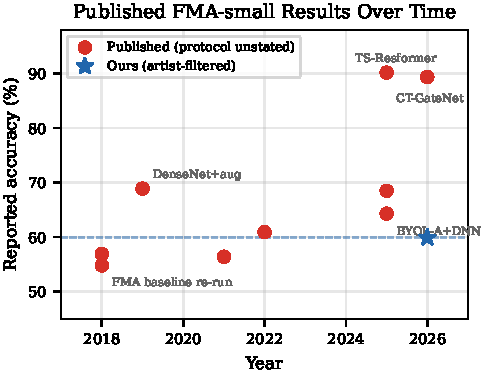
\includegraphics[width=\columnwidth]{literature_scatter.pdf}
\caption{Published FMA-small accuracies over time. Red circles denote results whose evaluation protocol is not stated; the blue star marks our artist-filtered CLAP probe (59.9\%). The dashed line marks our best overall result (AST Probe, 62.0\%). Results above the line are not necessarily better --- they may reflect a more permissive protocol.}
\label{fig:literature}
\end{figure}

One widely cited baseline --- "Defferrard et al., 58.0\%" ---
does not exist. The FMA paper\textquotesingle s only accuracy table
covers the 16-genre medium subset; 58 is the MLP cell there. The 54.8\%
attributed to FMA\textquotesingle s authors is actually Park et
al.\textquotesingle s re-run of FMA\textquotesingle s released baseline
code \citep{park2018representation}, artist-filtered by code inheritance
rather than authorial claim. We note that this attribution rests on code
inspection, not authorial statement --- a stronger basis than
accuracy inference but weaker than explicit protocol disclosure.

Since our original audit, we are not aware of any new FMA-small
publications that state their evaluation protocol. The reporting gap
persists.

\subsection{Data Leakage in Machine
Learning}\label{h.-data-leakage-in-machine-learning}

Data leakage --- the use of information during training that would
not be available at prediction time --- is a pervasive concern
across machine learning, not unique to audio. Kaufman et al.
\citep{kaufman2012leakage} formalised leakage types and proposed
detection methods, distinguishing between leakage through features
(training on test-set information) and leakage through examples
(inadequate train/test separation). Kapoor and Narayanan
\citep{kapoor2023leakage} surveyed 329 papers across 17 scientific
domains and found that data leakage affected a substantial fraction,
contributing to a broader reproducibility crisis in ML-based science.
Their finding confirms that the problem we document in MIR is not
field-specific but field-wide.

Source-level leakage is well understood in adjacent domains. Roberts et
al. \citep{roberts2017crossvalidation} demonstrated that standard random
cross-validation produces severely inflated performance estimates when
data has spatial, temporal, or hierarchical structure, and proposed
structured cross-validation strategies as remedies. In medical imaging,
Whalen et al. \citep{whalen2022navigating} documented how patient-level
splits are essential when multiple images come from the same patient;
failure to enforce this leads to models that recognise patients rather
than pathologies. The parallel to our setting is exact: replacing
"patient" with "artist" and "images" with "clips" yields an identical
formulation.

The pattern is consistent across fields: wherever data points share a
common origin, evaluation must split at the source level. Music genre
classification exhibits all three forms simultaneously --- the same
recording (clip-level), the same performance (track-level), and the same
production signature (artist-level). FMA ships the artist-level fix in
its metadata, but using it is optional and disclosing whether it was
used is rarer still.

Flexer and Schnitzer \citep{flexer2007closer} provided early evidence of
artist-filter effects in music classification, showing that removing the
artist confound significantly reduced classification accuracy on GTZAN.
Sturm \citep{sturm2014simple} went further, demonstrating that some MIR
systems functioned as "horses" --- exploiting dataset-specific
artifacts rather than learning musically meaningful features. Our
three-rung ladder provides the first systematic quantification of this
effect on FMA-small across multiple architectures.

The NeurIPS reproducibility checklist \citep{pineau2021neurips} now asks
about train/test contamination, representing an institutional attempt to
address leakage. However, the checklist does not specifically ask about
hierarchical source-level splitting --- the distinction between "are
your train and test sets disjoint?" (yes, by construction) and "are they
disjoint at the source level?" (often not). This gap means that a paper
can truthfully complete the checklist while still suffering from the
exact form of leakage we measure.

\subsection{Evaluation Protocol Reporting
Standards}\label{i.-evaluation-protocol-reporting-standards}

Institutional efforts to improve evaluation transparency have made
progress but leave significant gaps.

The \textbf{NeurIPS reproducibility checklist} \citep{pineau2021neurips}
asks authors to document dataset splits, specify whether existing splits
were used, and describe any preprocessing. These requirements are a step
forward, but they do not enforce hierarchical splitting. A paper can
truthfully report "we used an 80/10/10 random split" without mentioning
whether the randomisation operated at the clip, track, or artist level
--- and without triggering a checklist violation.

\textbf{ISMIR community practices} have historically been more attentive
to artist filtering than general ML venues, partly because the MIREX
evaluation campaigns standardise both tasks and data. However, MIREX
standardises by providing fixed splits, not by requiring papers to
disclose their split methodology when using their own data partitioning.
Papers published at ISMIR that use FMA-small with custom splits are not
required to state whether they artist-filter.

\textbf{MARBLE} \citep{yuan2024marble} and \textbf{HEAR}
\citep{turian2022hear} represent the benchmark approach: fix the split
so that all papers using the benchmark are comparable by construction.
This works within the benchmark but does not help when a paper uses a
standard dataset (like FMA-small) outside the benchmark framework.

The gap can be stated precisely: no major venue\textquotesingle s
submission checklist asks, "Does your train/test split control for
source-level identity (artist, patient, location)?" Until it does, the
protocol variable we measure --- worth 30+ points on FMA-small
--- will remain undisclosed by default.

\subsection{Training Techniques and
Regularisation}\label{j.-training-techniques-and-regularisation}

Several training techniques are relevant to our pipeline and merit brief
discussion for reproducibility.

\textbf{SpecAugment} \citep{park2019specaugment} applies random
frequency and time masks to mel spectrograms during training,
functioning as a regulariser that prevents the model from relying on
specific spectral regions or time intervals. Originally developed for
automatic speech recognition, it has become standard in audio
classification.

\textbf{Mixup} \citep{zhang2018mixup} interpolates between pairs of
training examples and their labels, encouraging models to behave
linearly between training samples. In our experiments, mixup with
alpha=0.3 consistently improves generalisation for probe models on
FMA-small.

\textbf{Label smoothing} \citep{szegedy2016rethinking} softens the hard
0/1 targets by redistributing a small fraction of probability mass to
non-target classes. With 8 balanced genres, label smoothing of 0.1
allocates approximately 0.014 to each non-target class, penalising
overconfident predictions.

\textbf{AdamW} \citep{loshchilov2019adamw} decouples weight decay from
the gradient update, providing more effective regularisation than L2
regularisation in the Adam optimiser. Combined with cosine annealing of
the learning rate, this forms our default optimisation setup.

\textbf{Focal loss} \citep{lin2017focal} down-weights well-classified
examples to concentrate training on hard cases. While designed for
class-imbalanced detection tasks, we evaluate it as an alternative to
cross-entropy for genres that are systematically hard to classify (Folk,
Experimental).

\section{Methodology}\label{methodology}

\subsection{Dataset}\label{a.-dataset}

FMA-small \citep{defferrard2017fma} contains 8,000 tracks (7,996
readable after excluding 4 corrupt files) balanced across eight genres:
Electronic, Experimental, Folk, Hip-Hop, Instrumental, International,
Pop, and Rock. Each track is approximately 30 seconds long. Following
standard practice in the FMA/GTZAN literature, each track is segmented
into ten non-overlapping 3-second episodes, yielding 75,296 total
episodes (60,188 train / 7,544 validation / 7,564 test).

\subsection{The Three-Rung Protocol
Ladder}\label{b.-the-three-rung-protocol-ladder}

We define three split modes to isolate each source of leakage:

\begin{enumerate}
\def\labelenumi{\arabic{enumi}.}
\item
  \textbf{Official (artist-filtered).} FMA\textquotesingle s shipped
  split. No artist appears in more than one partition. This is the only
  protocol used for headline results. Throughout this paper we refer to
  artist-filtered evaluation as the \emph{honest} protocol, meaning the
  protocol that prevents source-level identity leakage; the term carries
  no implication about the intent of researchers who use other splits.
\item
  \textbf{Random-track.} Random 80/10/10 over whole tracks. Artists may
  appear in multiple partitions, but clips from the same track stay
  together. This rung exists because most papers state "random 8:1:1"
  without naming the unit.
\item
  \textbf{Clip-random.} Random 80/10/10 over individual 3-second
  episodes (seed 42, genre-stratified). The same recording appears in
  both train and test. This is the most permissive protocol and produces
  the highest reported accuracies.
\end{enumerate}

The random-track and clip-random splits are generated once and cached;
all runs under a given protocol use the identical split. The
random-track split uses seed 42 with genre stratification.

\subsection{Track-Level Evaluation}\label{c.-track-level-evaluation}

All accuracies are track-level: per-episode softmax probabilities are
averaged within a track, then argmax selects the genre. This is stricter
than episode-level scoring and is the only unit we report, following the
principle that a 30-second track is the natural prediction target.

\subsection{Feature Extraction
Pipeline}\label{d.-feature-extraction-pipeline}

All representations are cached once and reused across experiments,
ensuring that backbone computation is not a variable between runs.

\textbf{Log-mel spectrograms.} For from-scratch CNN models, each
3-second episode is converted to a 128-bin log-mel spectrogram at 22,050
Hz (n\_fft=2048, hop\_length=512), yielding a 128 x 130 feature map.

\textbf{MERT embeddings.} MERT-v1-95M \citep{li2023mert} is a 12-layer
transformer pretrained on 20,000 hours of music via self-supervised
learning. We extract all 13 layer outputs (12 transformer + 1
convolutional projection), mean-pooled over the time dimension,
producing a (13, 768) tensor per episode. MERT-v1-330M (25 layers,
1024-dim) is extracted analogously. Audio is decoded at
MERT\textquotesingle s native 24 kHz via librosa
\citep{mcfee2015librosa}.

\textbf{MusicFM embeddings.} MusicFM \citep{li2024musicfm} extends the
wav2vec 2.0 framework with music-aware pretraining objectives. We
extract all layer outputs, mean-pooled over the time dimension,
producing a (13, 768) tensor per episode. Audio is decoded at 16 kHz.

\textbf{Wav2Vec 2.0 embeddings.} Wav2Vec 2.0-base
\citep{baevski2020wav2vec} is a 12-layer transformer pretrained via
contrastive learning on 960 hours of LibriSpeech. We extract all 13
layer outputs (12 transformer + 1 convolutional), mean-pooled over time,
producing a (13, 768) tensor per episode. Audio is decoded at 16 kHz.

\textbf{HuBERT embeddings.} HuBERT-base \citep{hsu2021hubert} uses the
same architecture as Wav2Vec 2.0 but is pretrained with
offline-clustered pseudo-labels on 960 hours of LibriSpeech. Extraction
is identical: (13, 768) per episode at 16 kHz.

\textbf{BEATs embeddings.} BEATs \citep{chen2023beats} combines audio
tokenisation with iterative self-supervised training, achieving
state-of-the-art on AudioSet. We extract all layer outputs, mean-pooled
over time, producing (13, 768) per episode at 16 kHz.

\textbf{Whisper encoder embeddings.} Whisper-small
\citep{radford2023whisper} is trained on 680,000 hours of web-scraped
speech for automatic speech recognition. We extract only the
encoder\textquotesingle s hidden states (discarding the decoder),
mean-pooled over time, producing (13, 768) per episode at 16 kHz.
Whisper has zero music-specific pretraining, serving as a control for
whether leakage is architecture-dependent or data-dependent.

\textbf{BYOL-A embeddings.} BYOL-A \citep{niizumi2023byola} produces a
single 2048-dimensional embedding per episode at 16 kHz.

\textbf{PANNs CNN14 embeddings.} PANNs CNN14 \citep{kong2020panns}
produces 2048-dimensional penultimate-layer embeddings per episode at 32
kHz.

\textbf{CLAP embeddings.} CLAP \citep{wu2023clap} learns aligned
audio-text representations via contrastive pretraining on audio-caption
pairs. We extract the audio encoder\textquotesingle s output, a single
512-dimensional vector per episode at 48 kHz. Only the audio encoder is
used during probing; the text encoder plays no role.

\textbf{EfficientAT embeddings.} EfficientAT MN10
\citep{schmid2023efficientat} is a lightweight CNN distilled from a
large audio transformer. We extract penultimate-layer features,
producing a 960-dimensional vector per episode at 32 kHz.

Table II summarises all backbones.

\begin{table*}[t]
\centering
\caption{Feature Extraction Summary: All Backbones}
\label{tab:backbones}
\footnotesize
\begin{tabular}{lccccc}
\toprule
\textbf{Backbone} & \textbf{Type} & \textbf{Params} & \textbf{Embed Shape} & \textbf{SR} & \textbf{Pretraining} \\
\midrule
Log-mel spectrogram & Hand-crafted & --- & (128, 130) & 22k & --- \\
MERT-v1-95M & Music SSL & 95M & (13, 768) & 24k & 20k hr music \\
MERT-v1-330M & Music SSL & 330M & (25, 1024) & 24k & 20k hr music \\
MusicFM & Music SSL & $\sim$95M & (13, 768) & 16k & Music \\
Wav2Vec 2.0-base & Speech SSL & 95M & (13, 768) & 16k & 960 hr speech \\
HuBERT-base & Speech SSL & 95M & (13, 768) & 16k & 960 hr speech \\
BEATs & Audio SSL & 90M & (13, 768) & 16k & AudioSet \\
Whisper-small enc. & Supervised ASR & 242M & (13, 768) & 16k & 680k hr speech \\
BYOL-A & Audio SSL & 5M & (2048,) & 16k & AudioSet \\
PANNs CNN14 & Supervised & 80M & (2048,) & 32k & AudioSet \\
CLAP & Audio-Language & 150M & (512,) & 48k & Audio+text \\
EfficientAT MN10 & Distilled CNN & 5M & (960,) & 32k & AudioSet (distill) \\
\bottomrule
\end{tabular}
\end{table*}

\subsection{Model Families}\label{e.-model-families}

We define probe architectures for all 12 backbones listed in Table II.
Frozen probing experiments are complete for six backbones (MERT-95M,
MERT-330M, BYOL-A, PANNs, CLAP, and log-mel CNNs) on a single Apple
M-series laptop. Additionally, fine-tuning and DGX-based probing
experiments cover AST, HTS-AT, EfficientAT, MERT (LoRA and partial
unfreeze), and Whisper, bringing the total to eight trained backbone
families spanning the following architecture families:

\textbf{From-scratch spectrogram models} consume 128-bin log-mel
spectrograms and train all parameters from scratch: GenreCNN (4-block
CNN, \textasciitilde260K params) \citep{choi2017transfer}, DenseNet121
(ImageNet-pretrained, adapted to single-channel input)
\citep{huang2017densenet, bian2019audio}.

\textbf{Music-specific SSL probes} train only a lightweight head on
cached embeddings from backbones pretrained specifically on music audio:

\begin{itemize}
\tightlist
\item
  \emph{MERT-95M learned weighted-sum probe} \citep{pasad2021layer}:
  softmax-weighted sum over all layers, followed by a two-layer MLP.
\item
  \emph{MERT-95M flat probe}: concatenates all 13 layers into a
  9,984-dim vector, followed by a two-layer MLP with LayerNorm.
\item
  \emph{MERT-95M deep probe} \citep{yang2021superb}: groups layers into
  multi-scale aggregations with residual blocks.
\item
  \emph{MERT-95M attention probe} \citep{safari2020self}: multi-head
  self-attention over the 13 layers with learnable positional
  embeddings.
\item
  \emph{MERT-330M probe}: learned weighted-sum with the 330M backbone.
\item
  \emph{MERT-330M flat probe}: 13-layer concatenation with the 330M
  backbone.
\item
  \emph{MERT-330M deep probe}: multi-scale aggregation with the 330M
  backbone.
\item
  \emph{MusicFM probe} \citep{li2024musicfm}: learned weighted-sum over
  MusicFM\textquotesingle s layer outputs, followed by a two-layer MLP.
\end{itemize}

\textbf{General audio and speech SSL probes} train only a lightweight
head on cached embeddings from backbones with no music-specific
pretraining objective:

\begin{itemize}
\tightlist
\item
  \emph{Wav2Vec 2.0 probe} \citep{baevski2020wav2vec}: learned
  weighted-sum over 13 layers, followed by a two-layer MLP.
\item
  \emph{HuBERT probe} \citep{hsu2021hubert}: same architecture as
  Wav2Vec 2.0 probe, on HuBERT embeddings.
\item
  \emph{BEATs probe} \citep{chen2023beats}: learned weighted-sum over
  layer outputs, followed by a two-layer MLP.
\item
  \emph{Whisper probe} \citep{radford2023whisper}: learned weighted-sum
  over encoder hidden states, followed by a two-layer MLP.
\item
  \emph{BYOL-A + DNN probe} \citep{niizumi2023byola}: LayerNorm followed
  by a variable-depth MLP on the 2048-dim BYOL-A embedding.
\item
  \emph{PANNs CNN14 probe} \citep{kong2020panns}: same architecture as
  BYOL-A probe, on PANNs 2048-dim embeddings.
\item
  \emph{CLAP probe} \citep{wu2023clap}: LayerNorm followed by a
  two-layer MLP on the 512-dim CLAP audio embedding.
\item
  \emph{EfficientAT probe} \citep{schmid2023efficientat}: LayerNorm
  followed by a two-layer MLP on the 960-dim EfficientAT embedding.
\end{itemize}

\textbf{Non-neural baseline.} XGBoost \citep{chen2016xgboost} on
flattened MERT embeddings (max\_depth=6, n\_estimators=256,
learning\_rate=0.1, subsample=0.8, colsample\_bytree=0.8; remaining
parameters at defaults).

\textbf{Fine-tuned models (DGX cluster).} End-to-end or
parameter-efficient fine-tuning of pretrained backbones, trained on
NVIDIA DGX hardware with bfloat16 mixed precision:

\begin{itemize}
\tightlist
\item
  \emph{AST-Finetune} \citep{gong2021ast}: AudioSet-pretrained Audio
  Spectrogram Transformer with layers 0--6 frozen and classifier
  fine-tuned. 10-second episodes at 16 kHz, batch size 32, learning rate
  1e-4, dropout 0.3, label smoothing 0.1, mixup 0.2.
\item
  \emph{MERT-LoRA-330M} \citep{li2023mert, hu2021lora}: LoRA adapters
  (rank=16, alpha=32, \textasciitilde2M trainable parameters) on the
  frozen MERT-v1-330M backbone. 3-second episodes at 24 kHz, batch size
  64, learning rate 2e-4, dropout 0.3, mixup 0.3.
\item
  \emph{MERT-LoRA-95M}: Same LoRA strategy on the smaller MERT-v1-95M
  backbone. Batch size 128, learning rate 3e-4.
\item
  \emph{MERT-Unfreeze-330M}: Top 4 transformer layers unfrozen with
  layer-wise learning rate decay (0.75x per layer). Batch size 32,
  learning rate 5e-5, dropout 0.4, weight decay 0.05.
\item
  \emph{MERT-MultiCrop-330M}: LoRA on MERT-330M with multi-crop
  processing --- 6 random 5-second crops during training, 10
  evenly-spaced crops at evaluation. Full 30-second tracks at 24 kHz,
  batch size 8.
\item
  \emph{HTS-AT-Genre} \citep{chen2022htsat}: Hierarchical Token-Semantic
  Audio Transformer (Swin-based, embed dim 96, depths {[}2,2,6,2{]},
  heads {[}3,6,12,24{]}) trained from scratch on FMA. 10-second episodes
  at 32 kHz, batch size 32, learning rate 3e-4, 60 epochs.
\item
  \emph{EfficientAT-Genre} \citep{schmid2023efficientat}: Lightweight
  EfficientAT (3M parameters) fine-tuned. 10-second episodes at 32 kHz,
  batch size 64, learning rate 3e-4.
\end{itemize}

\textbf{DGX probe models.} Layer-weighted MLP probes trained on DGX with
frozen backbone embeddings extracted at higher resolution and longer
context than the laptop probes:

\begin{itemize}
\tightlist
\item
  \emph{AST Probe}: Layer-weighted MLP over all 13 AST-AudioSet hidden
  layers (768-dim). 3 clips of 10 seconds each at 16 kHz.
\item
  \emph{Whisper Probe} \citep{radford2023whisper}: Layer-weighted MLP
  over Whisper-Large-v3 encoder states (1280-dim). Full 30-second audio
  at 16 kHz.
\item
  \emph{MERT-330M Probe (DGX)}: Layer-weighted MLP over 25 MERT-330M
  layers (1024-dim). 10 clips of 3 seconds each at 24 kHz.
\item
  \emph{Fusion Probe}: Concatenation of layer-averaged, normalised
  outputs from all four DGX encoders (AST, Whisper, MERT-330M, CLAP),
  producing a \textasciitilde4096-dim feature vector.
\item
  \emph{AST-V2}: Fine-tuned AST with SpecAugment, 3 random crops per
  epoch, freeze layers 0--4, learning rate 2e-5, mixup 0.4.
\end{itemize}

Separating music-specific from general-purpose backbones lets us test
whether music-aware pretraining provides any advantage under honest
evaluation --- or whether the apparent advantage in published
results reflects protocol choice rather than representation quality.

\subsection{Training Configuration}\label{f.-training-configuration}

All neural models use AdamW \citep{loshchilov2019adamw} with cosine
annealing. Spectrogram models apply SpecAugment
\citep{park2019specaugment} (2 frequency masks up to 16 bins, 2 time
masks up to 20 frames). Label smoothing (0.1)
\citep{szegedy2016rethinking} and mixup augmentation (alpha 0.3)
\citep{zhang2018mixup} are used for most runs. Early stopping with
patience 6--15 epochs prevents overfitting. Focal loss
\citep{lin2017focal} is evaluated as an alternative criterion.

Fine-tuned models on DGX use the same AdamW optimizer with cosine warmup
scheduling (200--500 warmup steps). Gradient clipping is set to
max\_grad\_norm = 1.0 for all fine-tuning runs. MERT-LoRA models use
gradient checkpointing to fit the 330M-parameter backbone in GPU memory.
All DGX training uses bfloat16 mixed precision (native on Hopper GPUs,
no loss scaling required). The Caruana forward selection ensemble
\citep{kittler1998combining} greedily adds models with replacement,
optimising validation track accuracy with log-loss as tie-breaker.

\subsection{Reproducibility
Statement}\label{g.-reproducibility-statement}

Frozen probing experiments run on a single Apple M-series laptop (MPS
backend, 16 GB RAM); embedding extraction takes 30--60 minutes per
backbone and probe training takes 1--3 minutes per run. Fine-tuning
and DGX probe experiments run on an NVIDIA DGX cluster with bfloat16
mixed precision; the seven Round 1 fine-tuning runs total approximately
6 GPU-hours. Total compute for the full study is under 50 GPU-hours
equivalent. All code, configurations, cached embeddings, and evaluation
scripts will be released upon publication. Every number in the results
section is mechanically generated from run artifacts by dedicated
scripts; no number is hand-edited. The embedding cache ensures exact
reproducibility of downstream experiments: given the same cached
features and random seed, training produces identical weights on the
same hardware.

\section{Experiments}\label{experiments}

We conducted 79 evaluated training runs: 54 under the artist-filtered
split (37 frozen probes on laptop, 7 fine-tuned models on DGX, 6 DGX
probes, and 4 ensemble configurations), 12 under random-track, and 13
under clip-random, spanning 21 unique architectures across eight
backbone families. Every result is mechanically generated from run
artifacts by dedicated scripts; no number in the results tables is
hand-edited.

\section{Results}\label{results}

\subsection{Best Model Per
Architecture}\label{a.-best-model-per-architecture}

Table III presents the best run per architecture (21 unique
architectures), ranked by accuracy under the artist-filtered,
track-level protocol. The table includes both frozen probes (trained on
laptop) and fine-tuned/DGX probe models.

\begin{table}[t]
\centering
\caption{Best Run Per Architecture (Artist-Filtered, Track-Level)}
\label{tab:best}
\scriptsize
\begin{tabular}{clccc}
\toprule
\textbf{\#} & \textbf{Architecture} & \textbf{Method} & \textbf{Acc.} & \textbf{F1} \\
\midrule
1 & R2 Ensemble (uniform) \cite{kittler1998combining} & Ens. & 62.1 & 62.0 \\
2 & AST Probe (DGX) \cite{gong2021ast} & Probe & 62.0 & --- \\
3 & R2 Ensemble (Caruana) \cite{kittler1998combining} & Ens. & 61.8 & 61.6 \\
4 & Fusion Probe (DGX) & Probe & 60.3 & --- \\
5 & CLAP probe \cite{wu2023clap} & Probe & 59.9 & 59.4 \\
6 & AST-V2 (fine-tuned) \cite{gong2021ast} & FT & 59.5 & --- \\
7 & R1 Ensemble (4-model) \cite{kittler1998combining} & Ens. & 58.9 & 58.8 \\
8 & R1 Ensemble (uniform) \cite{kittler1998combining} & Ens. & 58.5 & 58.2 \\
9 & MERT-95M flat probe \cite{li2023mert} & Probe & 58.2 & 57.8 \\
10 & AST-Finetune \cite{gong2021ast} & FT & 58.1 & 58.3 \\
11 & MERT-330M Probe (DGX) \cite{li2023mert} & Probe & 57.9 & --- \\
12 & BYOL-A + DNN probe \cite{niizumi2023byola} & Probe & 57.4 & 57.0 \\
13 & PANNs CNN14 probe \cite{kong2020panns} & Probe & 57.4 & 56.6 \\
14 & Whisper Probe (DGX) \cite{radford2023whisper} & Probe & 57.3 & --- \\
15 & MERT-330M probe \cite{li2023mert} & Probe & 56.6 & 56.5 \\
16 & EfficientAT-Genre \cite{schmid2023efficientat} & FT & 55.4 & 54.6 \\
17 & GenreCNN (log-mel) \cite{choi2017transfer} & Scratch & 55.1 & 54.2 \\
18 & MERT-LoRA-330M \cite{li2023mert,hu2021lora} & FT & 54.4 & 55.1 \\
19 & MERT-MultiCrop-330M \cite{li2023mert} & FT & 53.9 & 54.1 \\
20 & DenseNet121 \cite{huang2017densenet} & Scratch & 53.9 & 52.2 \\
21 & MERT-Unfreeze-330M \cite{li2023mert} & FT & 53.4 & 53.0 \\
22 & MERT-LoRA-95M \cite{li2023mert,hu2021lora} & FT & 52.9 & 51.9 \\
23 & XGBoost on MERT \cite{chen2016xgboost} & --- & 52.5 & 51.4 \\
24 & HTS-AT-Genre \cite{chen2022htsat} & Scratch & 47.4 & 47.0 \\
\bottomrule
\end{tabular}
\end{table}

\begin{figure}[t]
\centering
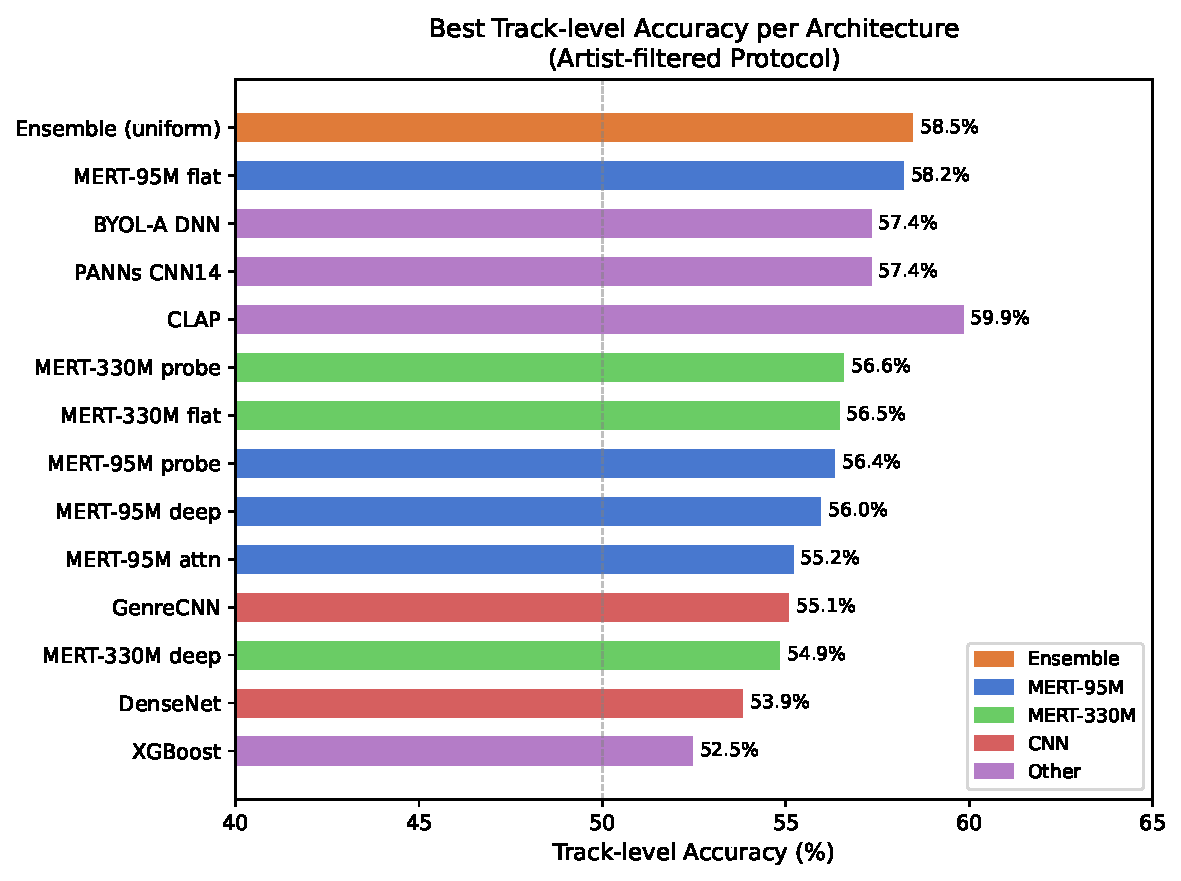
\includegraphics[width=\columnwidth]{architecture_bars.pdf}
\caption{Best track-level accuracy per architecture under the artist-filtered protocol. The AST Probe (62.0\%) leads, followed by the CLAP probe (59.9\%) and a cluster of MERT/BYOL-A/PANNs models at 57--58\%. Fine-tuned models (orange) do not consistently outperform frozen probes (blue).}
\label{fig:archbars}
\end{figure}

Figure \ref{fig:archbars} visualises these results. The best single
model is the AST Probe (62.0\%), a layer-weighted MLP on frozen
AudioSet-pretrained AST features trained on the DGX cluster. The best
laptop-trained model remains the CLAP probe (59.9\%), whose contrastive
audio-language pretraining produces representations that transfer
effectively to genre classification. A uniform-weight ensemble of all
Round 2 models reaches 62.1\%, marginally above the best individual.
Notably, fine-tuning does not consistently outperform frozen probing:
the frozen AST Probe (62.0\%) beats the fine-tuned AST (58.1\%), and
LoRA on MERT-330M (54.4\%) underperforms the frozen MERT-330M probe
(56.6\%). MERT-330M does not outperform MERT-95M, and learned ensemble
weights lose to fixed uniform averaging --- both symptoms of
overfitting at this data scale (6,400 training tracks).

\subsection{Complete Run Inventory}\label{b.-complete-run-inventory}

Table IV presents all 54 artist-filtered runs across the eight trained
backbone families, including hyperparameter variants, seed ablations,
and DGX fine-tuning experiments.

\begin{figure}[t]
\centering
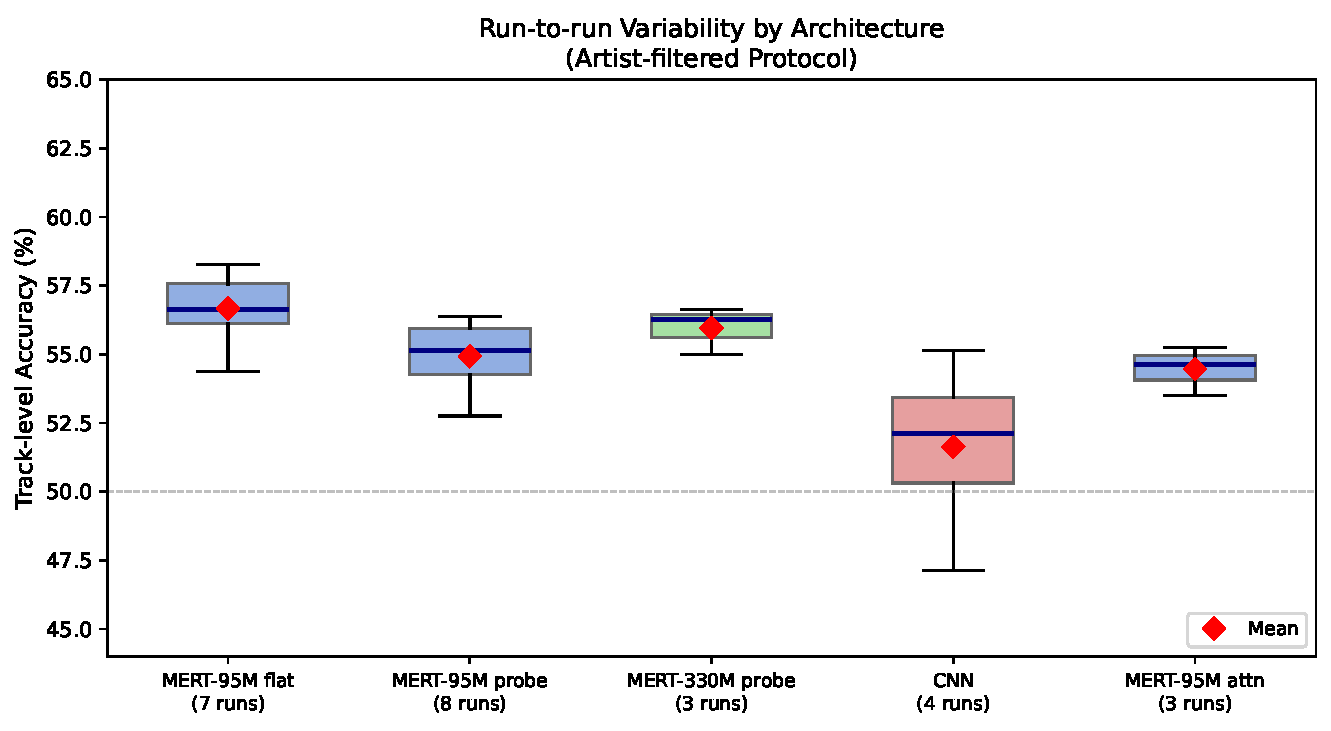
\includegraphics[width=\columnwidth]{seed_stability.pdf}
\caption{Run-to-run variability for architectures with multiple training runs. Box plots show median and quartiles; red diamonds mark means. The MERT Flat probe spans 3.8~pp across 7 runs differing only in seed and regularisation.}
\label{fig:seeds}
\end{figure}

\begin{figure*}[t]
\centering
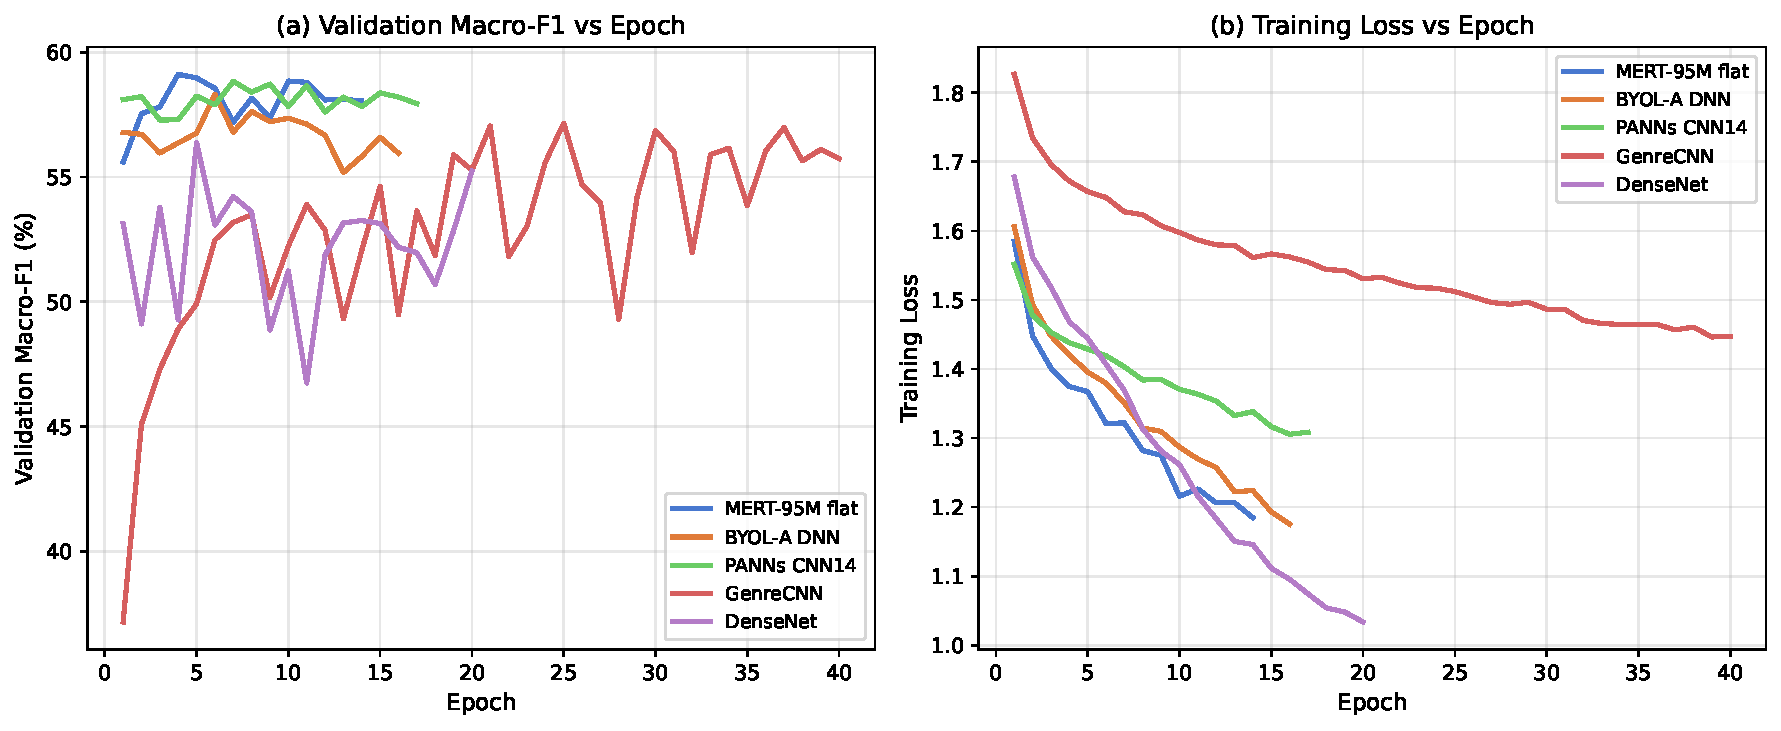
\includegraphics[width=\textwidth]{training_curves.pdf}
\caption{Training dynamics for five representative architectures. (a)~Validation macro-F1: probe models (MERT, BYOL-A, PANNs) converge in under 10 epochs; from-scratch models (GenreCNN, DenseNet) need 30--40. (b)~Training loss: probe losses plateau higher because the frozen backbone limits representational flexibility.}
\label{fig:curves}
\end{figure*}

The seed stability (Figure \ref{fig:seeds}) and training curves (Figure
\ref{fig:curves}) show key observations: (a) The MERT-95M flat probe
spans 54.4--58.2\% across 8 runs differing only in seed and
regularisation, a 3.9 pp range. (b) Seed ablations for the MERT-95M
probe (seeds 1--3, 42) span 53.5--56.4\%, showing that a 3 pp
difference between two papers could be seed noise. (c) The CNN baseline
improves from 47.1\% to 55.1\% (+8.0 pp) through augmentation and
hyperparameter tuning alone.

\begin{table*}[t]
\centering
\caption{Complete Inventory: All 54 Artist-Filtered Runs (Track-Level Accuracy and Macro-F1, \%). Rows 38--54 are DGX runs.}
\label{tab:allruns}
\scriptsize
\begin{tabular}{rllccccccl}
\toprule
\textbf{\#} & \textbf{Run} & \textbf{Architecture} & \textbf{Acc.} & \textbf{F1} & \textbf{LR} & \textbf{BS} & \textbf{Ep.} & \textbf{Drop.} & \textbf{Ref.} \\
\midrule
1 & clap\_probe\_v1 & CLAP probe & 59.9 & 59.4 & 3e-4 & 128 & 50 & 0.4 & \cite{wu2023clap} \\
2 & ensemble\_uniform & Ensemble (uniform avg) & 58.5 & 58.2 & --- & --- & --- & --- & \cite{kittler1998combining} \\
3 & ensemble\_weighted & Ensemble (weighted avg) & 58.2 & 58.1 & --- & --- & --- & --- & \cite{kittler1998combining} \\
4 & mert\_flat\_probe\_v1 & MERT-95M flat probe & 58.2 & 57.8 & 3e-4 & 128 & 50 & 0.5 & \cite{li2023mert} \\
5 & mert\_flat\_probe\_v2 & MERT-95M flat probe & 57.8 & 57.3 & 1e-4 & 64 & 50 & 0.6 & \cite{li2023mert} \\
6 & byola\_probe\_v1 & BYOL-A + DNN probe & 57.4 & 57.0 & 3e-4 & 128 & 50 & 0.4 & \cite{niizumi2023byola} \\
7 & mert\_flat\_diverse\_s3 & MERT-95M flat probe & 57.4 & 56.5 & 2e-4 & 128 & 50 & 0.6 & \cite{li2023mert} \\
8 & panns\_probe\_v1 & PANNs CNN14 probe & 57.4 & 56.6 & 3e-4 & 128 & 50 & 0.4 & \cite{kong2020panns} \\
9 & mert\_flat\_diverse\_s4 & MERT-95M flat probe & 56.6 & 56.1 & 2e-4 & 128 & 50 & 0.5 & \cite{li2023mert} \\
10 & mert\_large\_probe\_v1 & MERT-330M probe & 56.6 & 56.5 & 5e-4 & 128 & 50 & 0.4 & \cite{li2023mert} \\
11 & mert\_flat\_diverse\_s1 & MERT-95M flat probe & 56.5 & 55.8 & 3e-4 & 128 & 50 & 0.5 & \cite{li2023mert} \\
12 & mert\_large\_flat\_v1 & MERT-330M flat probe & 56.5 & 55.9 & 1e-4 & 64 & 50 & 0.6 & \cite{li2023mert} \\
13 & mert\_probe\_tuned & MERT-95M probe (learned wt.) & 56.4 & 55.7 & 2e-4 & 64 & 60 & 0.5 & \cite{pasad2021layer} \\
14 & mert\_large\_probe\_v3 & MERT-330M probe & 56.2 & 56.2 & 1e-4 & 128 & 50 & 0.3 & \cite{li2023mert} \\
15 & mert\_probe\_wide & MERT-95M probe (learned wt.) & 56.1 & 55.3 & 5e-4 & 128 & 40 & 0.4 & \cite{pasad2021layer} \\
16 & mert\_deep\_probe\_v2 & MERT-95M deep probe & 56.0 & 55.9 & 1e-4 & 64 & 60 & 0.5 & \cite{yang2021superb} \\
17 & mert\_flat\_diverse\_s6 & MERT-95M flat probe & 56.0 & 55.4 & 2.5e-4 & 128 & 50 & 0.55 & \cite{li2023mert} \\
18 & mert\_probe\_baseline & MERT-95M probe (learned wt.) & 55.9 & 54.9 & 1e-3 & 256 & 40 & 0.3 & \cite{pasad2021layer} \\
19 & mert\_flat\_diverse\_s5 & MERT-95M flat probe & 55.8 & 55.6 & 4e-4 & 128 & 50 & 0.4 & \cite{li2023mert} \\
20 & mert\_deep\_probe\_v1 & MERT-95M deep probe & 55.5 & 55.0 & 3e-4 & 128 & 60 & 0.4 & \cite{yang2021superb} \\
21 & mert\_attn\_probe\_v2 & MERT-95M attention probe & 55.2 & 54.4 & 5e-4 & 128 & 60 & 0.4 & \cite{safari2020self} \\
22 & mert\_probe\_seed2 & MERT-95M probe (seed 2) & 55.2 & 55.0 & 5e-4 & 128 & 40 & 0.4 & \cite{pasad2021layer} \\
23 & cnn\_improved & GenreCNN (log-mel) & 55.1 & 54.2 & 3e-4 & 32 & 60 & --- & \cite{choi2017transfer} \\
24 & mert\_large\_probe\_v2 & MERT-330M probe & 55.0 & 55.0 & 3e-4 & 64 & 50 & 0.5 & \cite{li2023mert} \\
25 & mert\_probe\_deep & MERT-95M probe (deep head) & 55.0 & 54.4 & 1e-4 & 256 & 80 & 0.5 & \cite{pasad2021layer} \\
26 & mert\_large\_deep\_v1 & MERT-330M deep probe & 54.9 & 55.5 & 3e-4 & 64 & 50 & 0.4 & \cite{yang2021superb} \\
27 & mert\_attn\_probe\_v1 & MERT-95M attention probe & 54.6 & 53.6 & 3e-4 & 128 & 60 & 0.3 & \cite{safari2020self} \\
28 & mert\_probe\_seed3 & MERT-95M probe (seed 3) & 54.5 & 54.4 & 5e-4 & 128 & 40 & 0.4 & \cite{pasad2021layer} \\
29 & mert\_flat\_diverse\_s2 & MERT-95M flat probe & 54.4 & 53.7 & 3e-4 & 128 & 50 & 0.5 & \cite{li2023mert} \\
30 & densenet\_v1 & DenseNet121 & 53.9 & 52.2 & 3e-4 & 32 & 60 & 0.3 & \cite{huang2017densenet} \\
31 & mert\_attn\_probe\_v3 & MERT-95M attention probe & 53.5 & 52.8 & 1e-4 & 64 & 60 & 0.2 & \cite{safari2020self} \\
32 & mert\_probe\_seed1 & MERT-95M probe (seed 1) & 53.5 & 52.9 & 5e-4 & 128 & 40 & 0.4 & \cite{pasad2021layer} \\
33 & cnn\_tuned\_lr & GenreCNN (log-mel) & 52.9 & 52.2 & 3e-4 & 32 & 35 & --- & \cite{choi2017transfer} \\
34 & mert\_probe\_lastlayer & MERT-95M probe (last layer) & 52.8 & 51.8 & 1e-3 & 256 & 40 & 0.3 & \cite{pasad2021layer} \\
35 & xgboost\_mert & XGBoost on MERT & 52.5 & 51.4 & --- & 256 & --- & --- & \cite{chen2016xgboost} \\
36 & cnn\_augmented & GenreCNN (log-mel) & 51.4 & 50.4 & 1e-3 & 64 & 30 & --- & \cite{choi2017transfer} \\
37 & cnn\_baseline & GenreCNN (log-mel) & 47.1 & 45.0 & 1e-3 & 64 & 25 & --- & \cite{choi2017transfer} \\
\midrule
\multicolumn{10}{l}{\textit{DGX Fine-Tuned Models (Round 1)}} \\
\midrule
38 & ast\_finetune & AST-Finetune (freeze 6/12) & 58.1 & 58.3 & 1e-4 & 32 & 1 & 0.3 & \cite{gong2021ast} \\
39 & efficientat\_genre & EfficientAT-Genre & 55.4 & 54.6 & 3e-4 & 64 & 41 & --- & \cite{schmid2023efficientat} \\
40 & mert\_lora\_330m & MERT-LoRA-330M & 54.4 & 55.1 & 2e-4 & 64 & 2 & 0.3 & \cite{li2023mert,hu2021lora} \\
41 & mert\_multicrop\_330m & MERT-MultiCrop-330M & 53.9 & 54.1 & 2e-4 & 8 & 10 & --- & \cite{li2023mert} \\
42 & mert\_unfreeze\_330m & MERT-Unfreeze-330M & 53.4 & 53.0 & 5e-5 & 32 & 8 & 0.4 & \cite{li2023mert} \\
43 & mert\_lora\_95m & MERT-LoRA-95M & 52.9 & 51.9 & 3e-4 & 128 & 19 & 0.3 & \cite{li2023mert,hu2021lora} \\
44 & htsat\_genre & HTS-AT-Genre (from scratch) & 47.4 & 47.0 & 3e-4 & 32 & 28 & --- & \cite{chen2022htsat} \\
\midrule
\multicolumn{10}{l}{\textit{DGX Probes and Fine-Tuned Models (Round 2)}} \\
\midrule
45 & probe\_ast & AST Probe (layer-weighted) & 62.0 & --- & --- & --- & --- & --- & \cite{gong2021ast} \\
46 & probe\_fusion & Fusion Probe (4 encoders) & 60.3 & --- & --- & --- & --- & --- & --- \\
47 & ast\_v2 & AST-V2 (fine-tuned) & 59.5 & --- & 2e-5 & 32 & 3 & --- & \cite{gong2021ast} \\
48 & probe\_mert & MERT-330M Probe (DGX) & 57.9 & --- & --- & --- & --- & --- & \cite{li2023mert} \\
49 & probe\_whisper & Whisper Probe (DGX) & 57.3 & --- & --- & --- & --- & --- & \cite{radford2023whisper} \\
50 & probe\_clap & CLAP Probe (DGX) & 27.8 & --- & --- & --- & --- & --- & \cite{wu2023clap} \\
\midrule
\multicolumn{10}{l}{\textit{DGX Ensembles}} \\
\midrule
51 & r2\_ensemble\_uniform & R2 Ensemble (uniform all) & 62.1 & 62.0 & --- & --- & --- & --- & \cite{kittler1998combining} \\
52 & r2\_ensemble\_caruana & R2 Ensemble (Caruana) & 61.8 & 61.6 & --- & --- & --- & --- & \cite{kittler1998combining} \\
53 & r1\_ensemble\_4model & R1 Ensemble (4-model) & 58.9 & 58.8 & --- & --- & --- & --- & \cite{kittler1998combining} \\
54 & r1\_ensemble\_7model & R1 Ensemble (7-model) & 58.5 & 58.2 & --- & --- & --- & --- & \cite{kittler1998combining} \\
\bottomrule
\end{tabular}
\end{table*}

\subsection{Protocol Leakage
Ladder}\label{c.-protocol-leakage-ladder}

Table V combines the three protocols for the 11 architectures tested on
all three rungs.

\begin{table*}[t]
\centering
\caption{Protocol Leakage Ladder: Identical Architectures Under Three Split Protocols (Track-Level Accuracy, \%)}
\label{tab:leakage}
\footnotesize
\begin{tabular}{lcccc}
\toprule
\textbf{Model} & \textbf{Artist-filtered} & \textbf{Random-track} & \textbf{Clip-random} & \textbf{Inflation (pp)} \\
\midrule
MERT Probe (weighted-sum) \cite{pasad2021layer} & 56.1 & 69.2 & 93.6 & +37.5 \\
MERT Flat Probe (13-layer) \cite{li2023mert} & 58.2 & 70.2 & 90.2 & +32.0 \\
MERT Deep Probe (multi-scale) \cite{yang2021superb} & 55.5 & 68.5 & 92.2 & +36.7 \\
MERT Attention Probe \cite{safari2020self} & 54.6 & 69.8 & 95.7 & +41.0 \\
MERT-330M Probe \cite{li2023mert} & 56.6 & 70.9 & 96.0 & +39.4 \\
MERT-330M Flat Probe \cite{li2023mert} & 56.5 & 71.2 & 91.9 & +35.4 \\
MERT-330M Deep Probe \cite{yang2021superb} & 54.9 & 69.0 & 96.1 & +41.2 \\
CNN (log-mel spectrogram) \cite{choi2017transfer} & 55.1 & 62.9 & 69.2 & +14.1 \\
BYOL-A + DNN \cite{niizumi2023byola} & 57.4 & 69.9 & 84.5 & +27.2 \\
PANNs CNN14 \cite{kong2020panns} & 57.4 & 67.2 & 73.4 & +16.0 \\
CLAP \cite{wu2023clap} & 59.9 & 71.8 & 78.6 & +18.7 \\
\midrule
\textbf{Mean (11 verified)} & \textbf{56.6} & \textbf{69.1} & \textbf{87.4} & \textbf{+30.8} \\
\bottomrule
\end{tabular}
\end{table*}

\begin{figure*}[t]
\centering
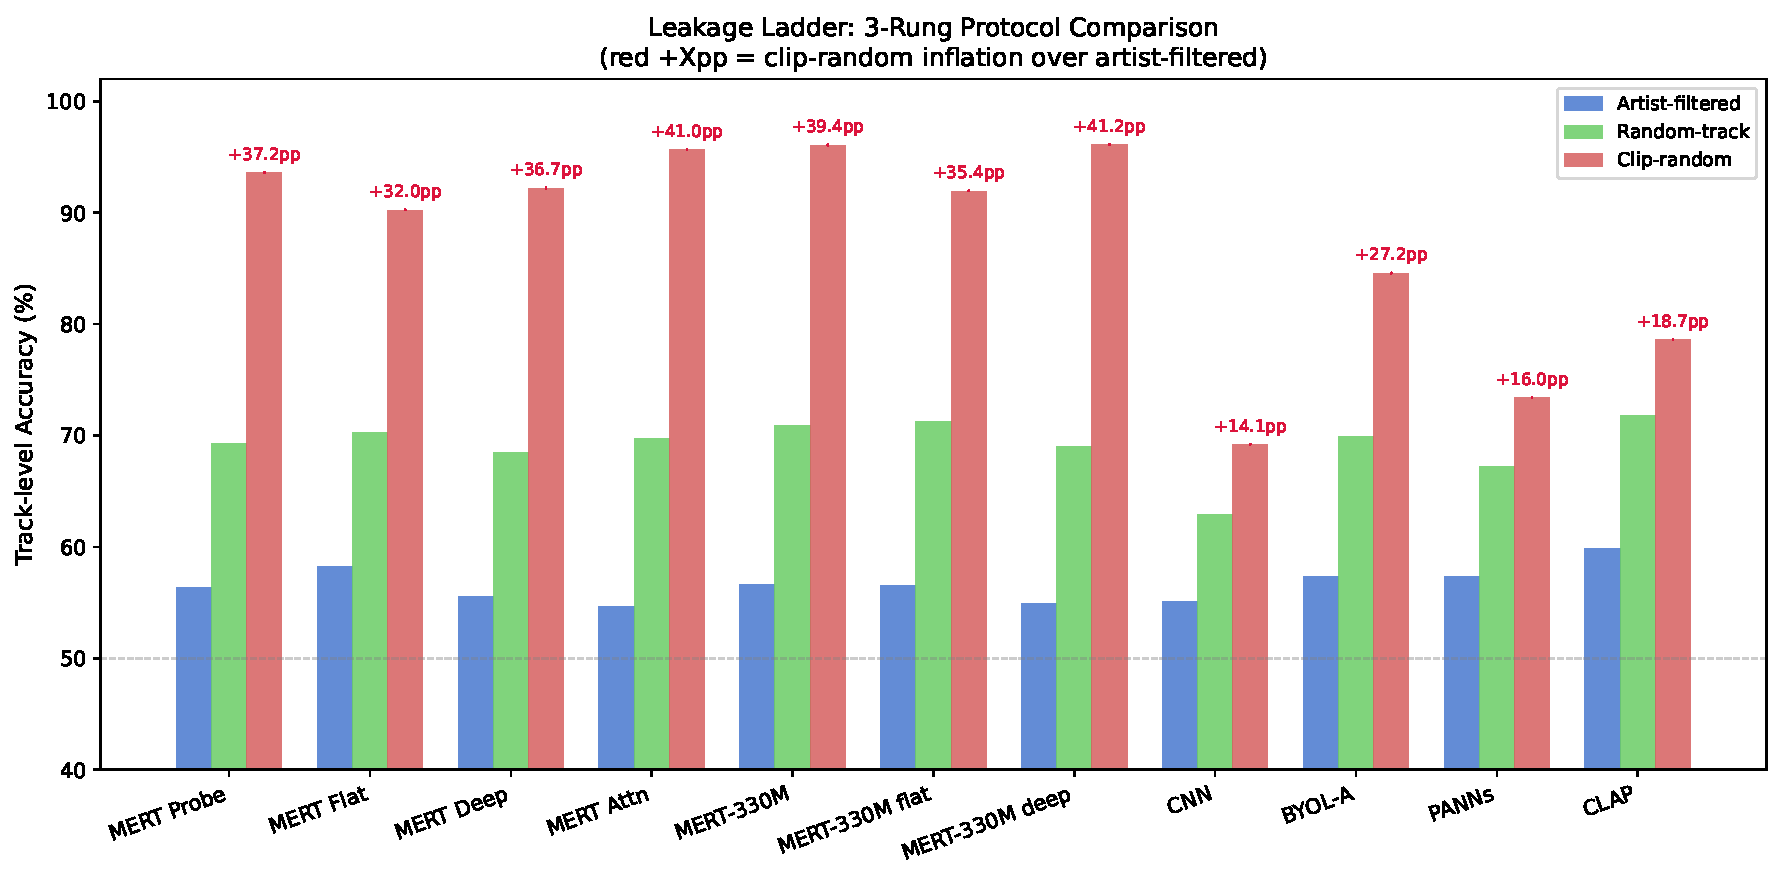
\includegraphics[width=\textwidth]{leakage_bars.pdf}
\caption{Protocol leakage across all 11 verified architectures. Blue bars show artist-filtered accuracy; orange bars show random-track; red bars show clip-random. Red annotations above each bar show the total inflation in percentage points. The MERT-330M deep probe inflates by +41~pp --- from 54.9\% to 96.1\%.}
\label{fig:leakage}
\end{figure*}

Figure \ref{fig:leakage} shows the full ladder. Decomposed (over the 7
architectures with all three rungs): dropping the artist filter alone
accounts for +12.6 pp, and leaking clips on top adds +18.3 pp (total
+30.9 pp for this subset; the headline +30.8 pp is the mean across all
11 architectures with at least the two extreme rungs). The effect is
systematic and architecture-independent.

\subsection{Genre-Specific Leakage
Analysis}\label{d.-genre-specific-leakage-analysis}

\begin{figure}[t]
\centering
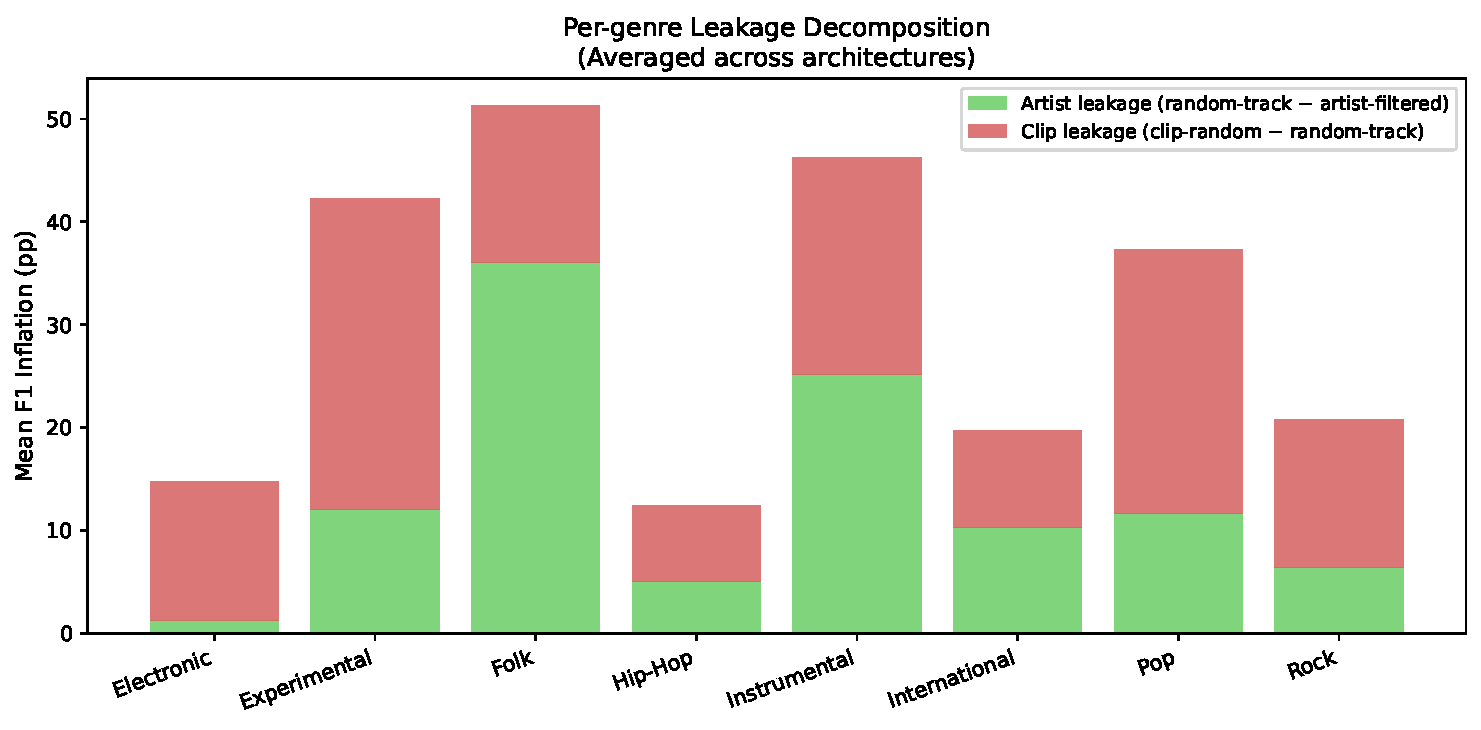
\includegraphics[width=\columnwidth]{genre_leakage_decomposition.pdf}
\caption{Per-genre leakage decomposition, averaged across 8 architectures. Genres are sorted by total inflation (clip-random minus artist-filtered). Folk inflates by +49.8~pp; Hip-Hop by only +14.0~pp. The orange segment isolates artist leakage; the red segment isolates clip leakage on top of that.}
\label{fig:genre_decomp}
\end{figure}

\begin{figure}[t]
\centering
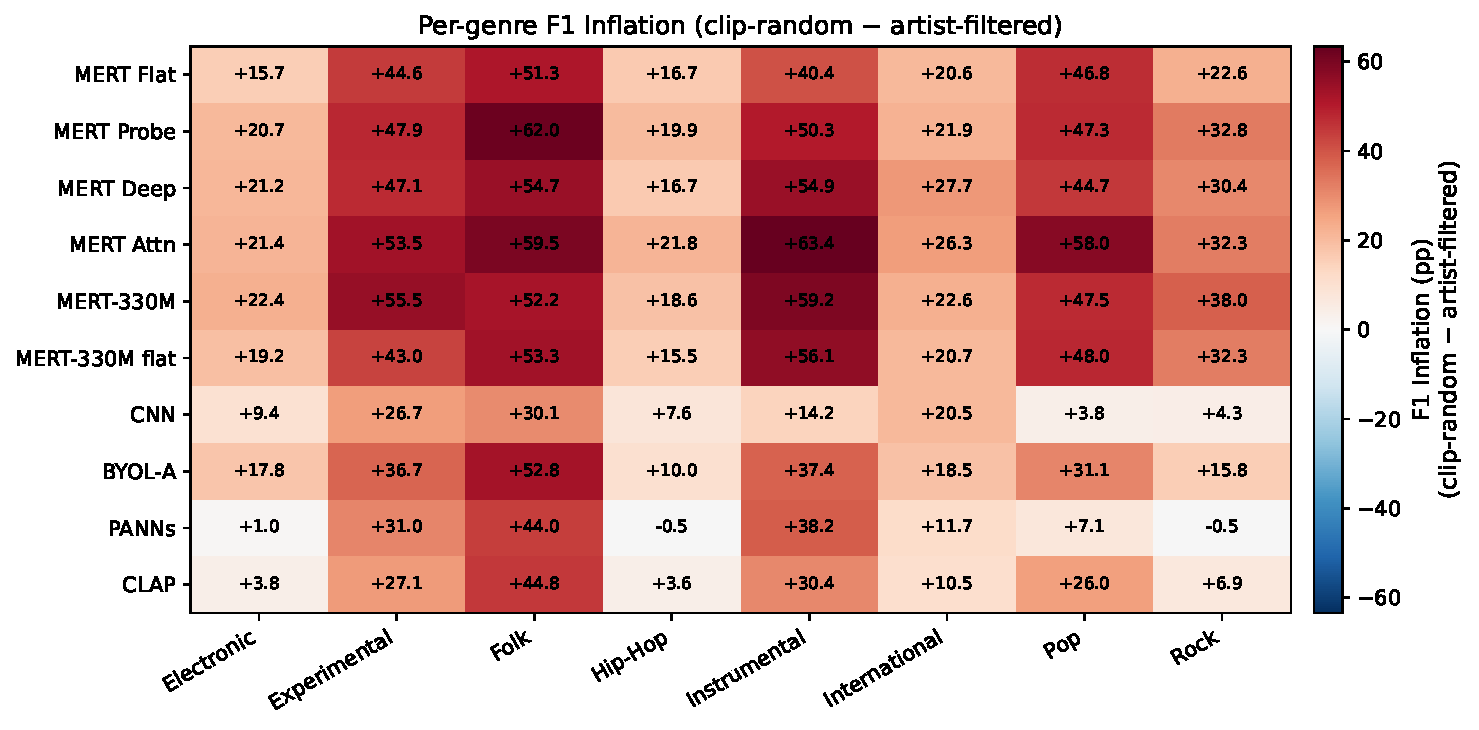
\includegraphics[width=\columnwidth]{genre_inflation_heatmap.pdf}
\caption{Genre-specific inflation (pp) for each architecture. Dark cells indicate high inflation. Folk and Instrumental are consistently the most inflated genres; Hip-Hop and Electronic are the least. The MERT attention probe on Instrumental inflates by +63~pp.}
\label{fig:genre_heatmap_infl}
\end{figure}

\begin{figure}[t]
\centering
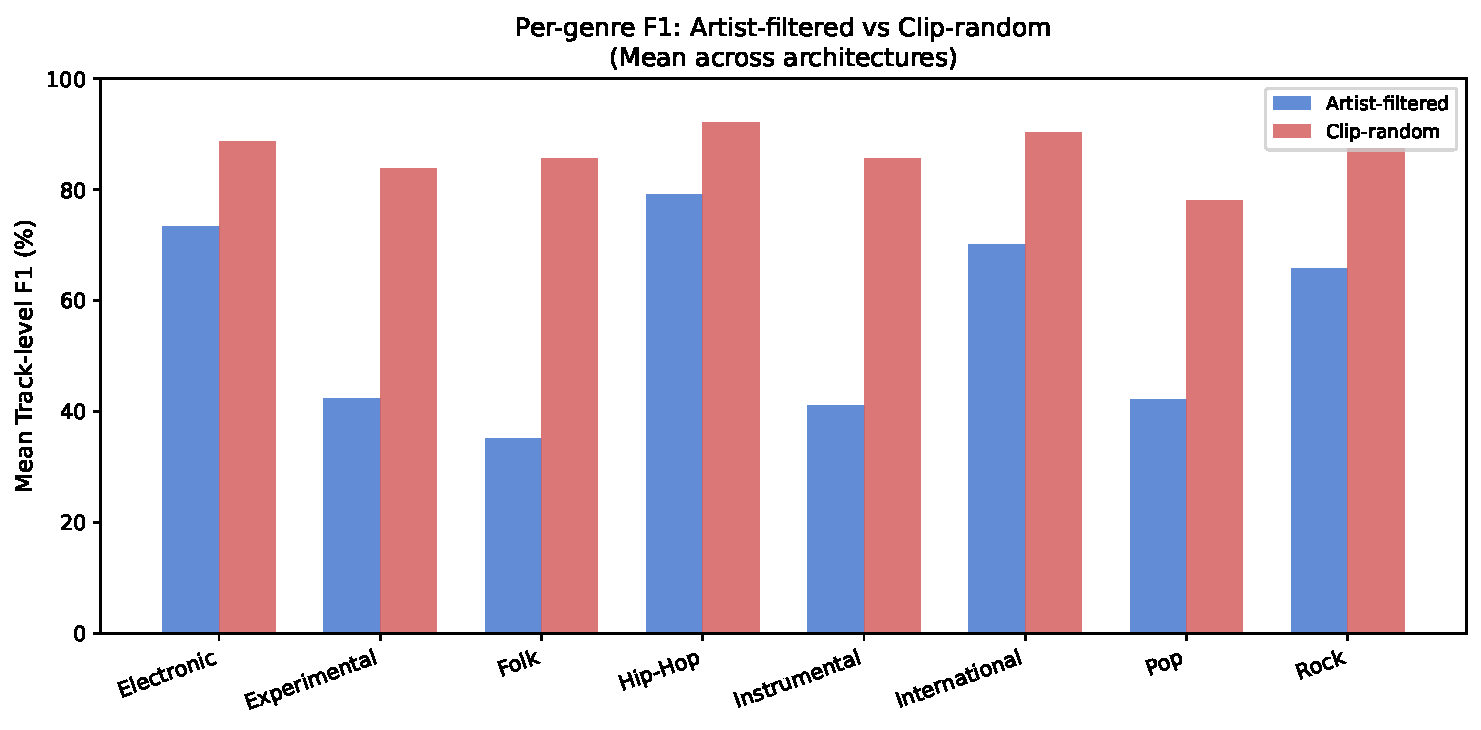
\includegraphics[width=\columnwidth]{genre_inflation_bars.pdf}
\caption{Per-genre inflation (mean across architectures). Blue: artist-filtered F1; red: clip-random F1. The gap measures how much each genre benefits from leaky evaluation. Folk (+50~pp) and Instrumental (+45~pp) are most inflated.}
\label{fig:genre_bars}
\end{figure}

Figures \ref{fig:genre_decomp}--\ref{fig:genre_bars} show that not all
genres inflate equally. Folk (+49.8 pp mean inflation), Instrumental
(+45.2 pp), and Experimental (+42.8 pp) inflate the most. These are also
the three hardest genres under honest evaluation (36.1\%, 40.9\%, and
41.4\% mean F1 respectively). The explanation: these genres are
stylistically diffuse, so models learn to recognise \emph{which
recording} they have heard rather than genre features. Hip-Hop (+14.0
pp) and Electronic (+16.3 pp) inflate the least, having strong acoustic
signatures that transfer across artists.

\begin{figure*}[t]
\centering
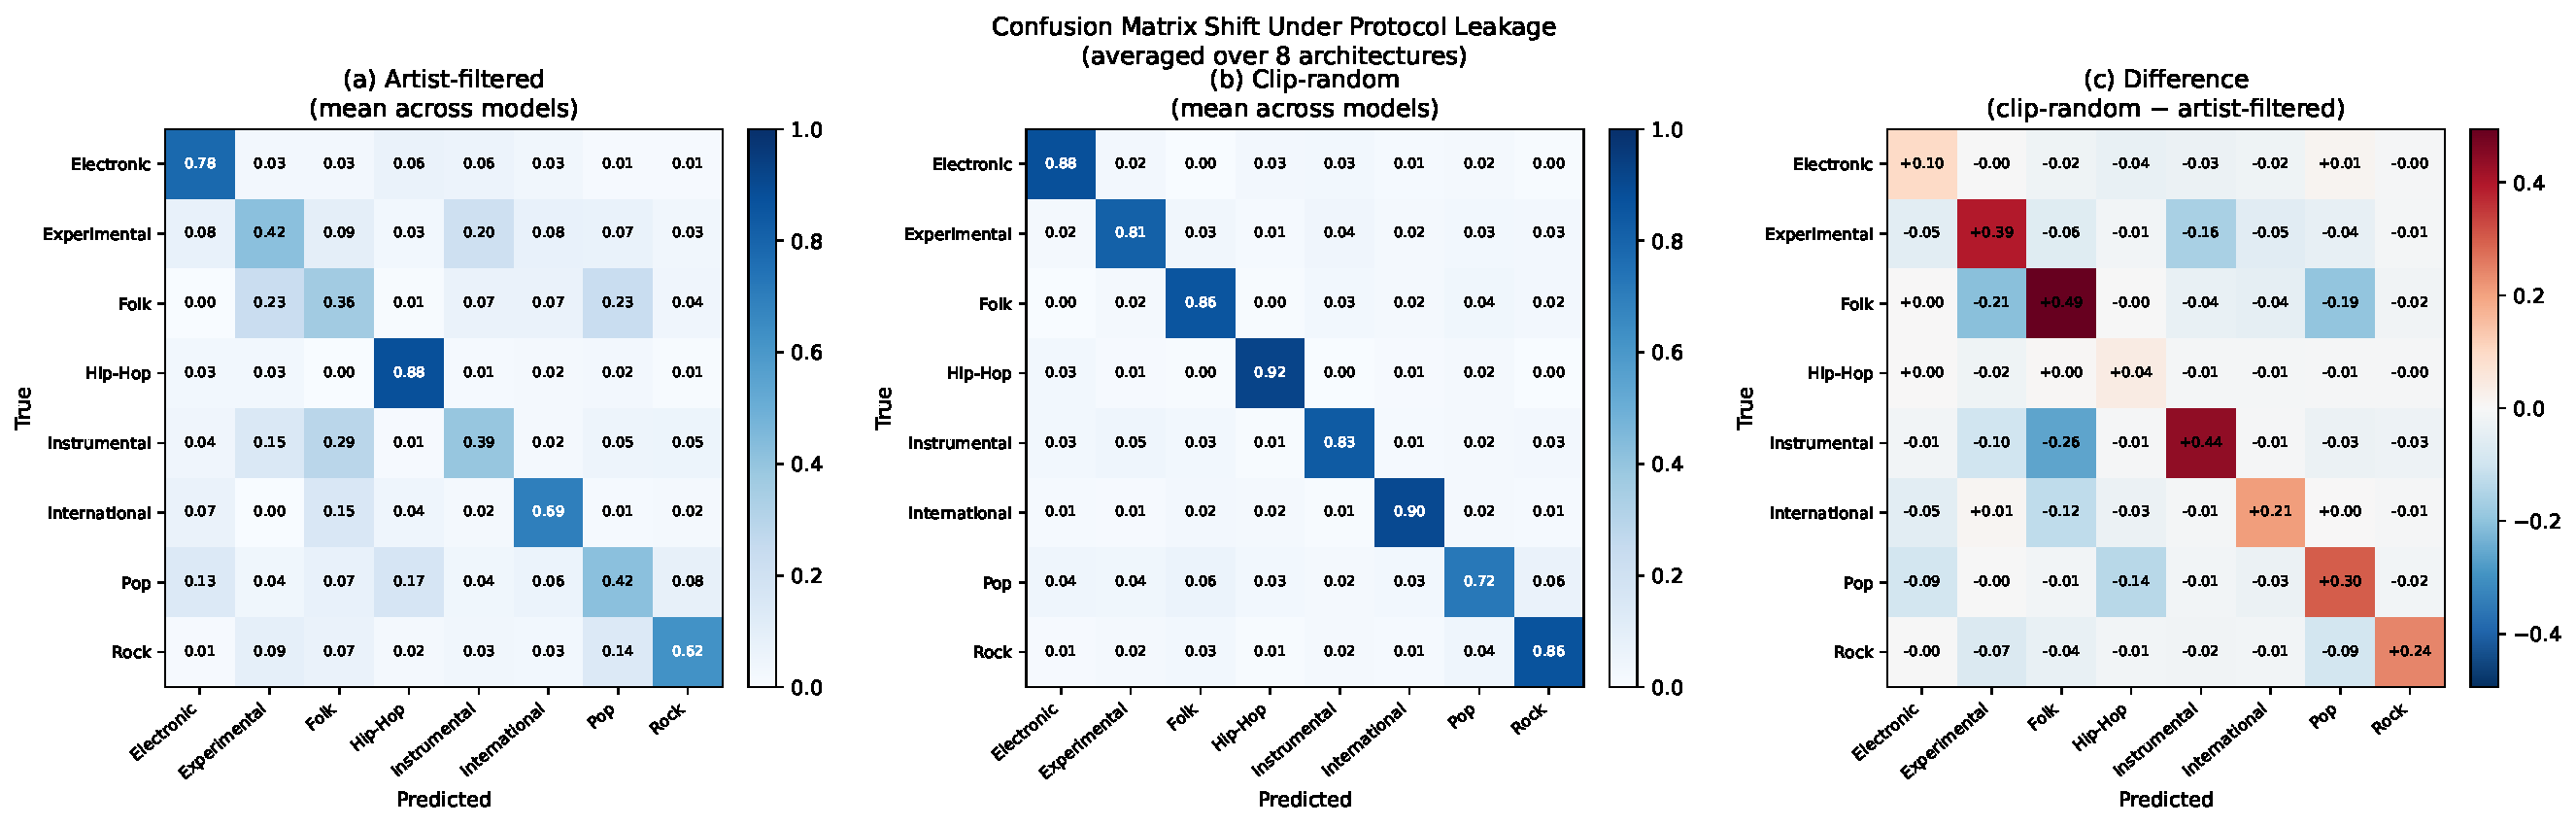
\includegraphics[width=\textwidth]{confusion_diff.pdf}
\caption{Confusion matrix shift under protocol leakage, averaged across 8 architectures. (a) Artist-filtered: off-diagonal mass in Folk$\rightarrow$Experimental (22.8\%), Instrumental$\rightarrow$Folk (28.6\%), and Pop$\rightarrow$Hip-Hop (16.5\%) reflects genuine genre ambiguity. (b) Clip-random: confusion collapses as models recognise recordings. (c) Difference: diagonal gains (recording recognition) come at the expense of off-diagonal confusion (genre ambiguity). Folk gains +49.4~pp on-diagonal; the largest off-diagonal reduction is Instrumental$\rightarrow$Folk ($-25.9$~pp).}
\label{fig:confusion_diff}
\end{figure*}

The confusion matrix shift (Figure \ref{fig:confusion_diff}) reveals
\emph{what} leakage fixes. Under honest evaluation, the dominant
confusions are between acoustically similar genres:
Instrumental\(\rightarrow\)Folk (28.6\%),
Folk\(\rightarrow\)Experimental (22.8\%), and Folk\(\rightarrow\)Pop
(23.1\%). Under clip-random evaluation, these confusions nearly vanish
--- not because the model learned genre boundaries, but because it
learned recording identities. The off-diagonal reductions are not a sign
of better generalisation; they are a sign of memorisation replacing
classification.

\subsection{Cross-Architecture Leakage
Consistency}\label{e.-cross-architecture-leakage-consistency}

To test whether the leakage pattern is architecture-independent, we
compute the Spearman rank correlation between per-genre inflation
vectors across all architecture pairs. Each architecture produces an
8-element vector of per-genre inflation values (clip-random F1 minus
artist-filtered F1). If the genre vulnerability ordering is consistent
across architectures, the pairwise rank correlations should be high.

Across the 11 verified architectures, the genre vulnerability ordering
is remarkably consistent: Folk, Instrumental, and Experimental inflate
the most, while Hip-Hop and Electronic inflate the least. This stability
confirms that the inflation pattern is a property of the
dataset\textquotesingle s genre structure and the evaluation protocol,
not of any particular learned representation.

The stability of the genre vulnerability ordering has a practical
implication: if Folk and Instrumental are always the most inflated
genres, then a paper\textquotesingle s reported per-genre accuracy
profile can serve as a soft diagnostic for protocol choice. A model that
achieves 85\% on Folk under an unstated protocol is more likely using a
permissive split than one that achieves 85\% on Hip-Hop.

\subsection{Audio-Language Models:
CLAP}\label{f.-audio-language-models-clap}

CLAP \citep{wu2023clap} approaches audio understanding through
contrastive language-audio pretraining, learning a joint embedding space
where audio and text descriptions are aligned. Its 512-dimensional audio
embeddings encode semantic content at a higher level of abstraction than
purely acoustic models. Under the artist-filtered protocol, the laptop
CLAP probe achieves 59.9\% track-level accuracy --- the best among
laptop-trained models, surpassing MERT-95M (58.2\%) and the laptop
uniform ensemble (58.5\%). The DGX AST Probe (62.0\%) now leads overall
(Section G2), but CLAP\textquotesingle s strong frozen-probe performance
demonstrates that audio-language pretraining on diverse audio-text pairs
produces representations that transfer remarkably well to music genre
classification.

The CLAP leakage pattern (+18.7 pp inflation) is notably lower than the
MERT family (+32--41 pp) but higher than the from-scratch CNN (+14.1
pp). This intermediate position is consistent with
CLAP\textquotesingle s pretraining: its contrastive objective encourages
semantic invariance across acoustic variations, which may reduce
recording-specific memorisation compared to reconstruction-based
objectives (MERT) while still capturing more fine-grained features than
a shallow CNN.

Whisper Probe results from the DGX experiments (57.3\%) provide initial
evidence on speech-only models applied to music: despite never
encountering music during pretraining, Whisper\textquotesingle s encoder
representations transfer competently to genre classification, though
below the best music-specific and AudioSet-pretrained models.

\subsection{Against Published
Literature}\label{g.-against-published-literature}

Our best artist-filtered model reaches 62.0\% (per-genre breakdown in
Figure \ref{fig:heatmap}; confusion matrices in Figures
\ref{fig:confusion_af}--\ref{fig:confusion_cr}). The only published
number carrying an artist-filtered guarantee is 54.8\% (Park et
al.\textquotesingle s re-run of FMA\textquotesingle s baseline code
\citep{park2018representation}), a margin of +7.2 pp. We deliberately do
not report a "beats N of M" count: ranking against numbers whose
protocol is unknown would treat incomparable quantities as comparable.

\begin{figure}[t]
\centering
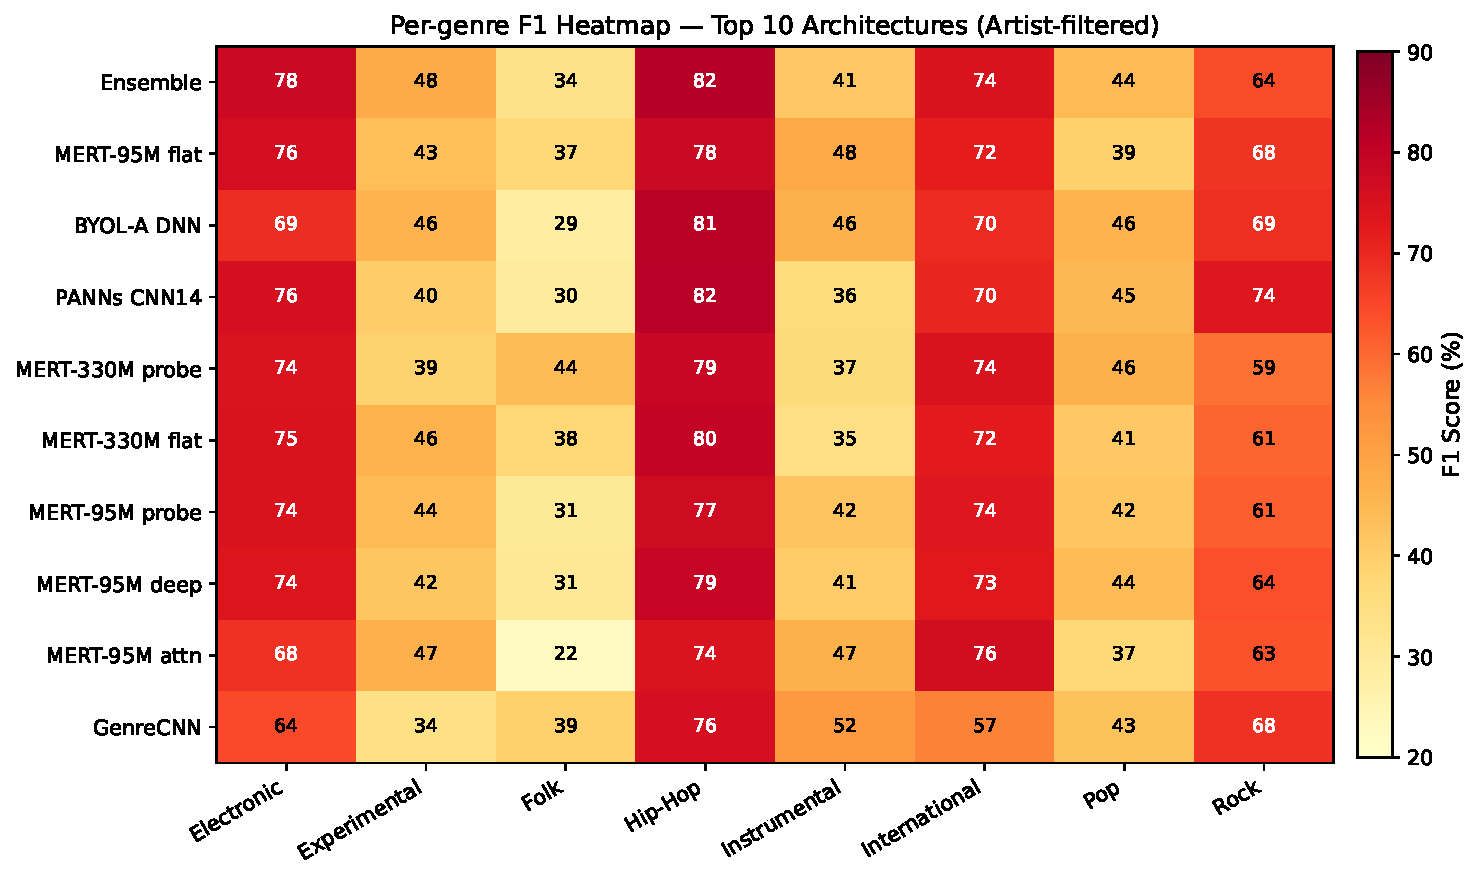
\includegraphics[width=\columnwidth]{genre_heatmap.pdf}
\caption{Per-genre F1 (\%) across the ten best architectures. Hip-Hop and Electronic are consistently well-classified (76--82\%); Folk and Pop are hardest (26--44\%), likely due to stylistic overlap with other genres.}
\label{fig:heatmap}
\end{figure}

\begin{figure}[t]
\centering
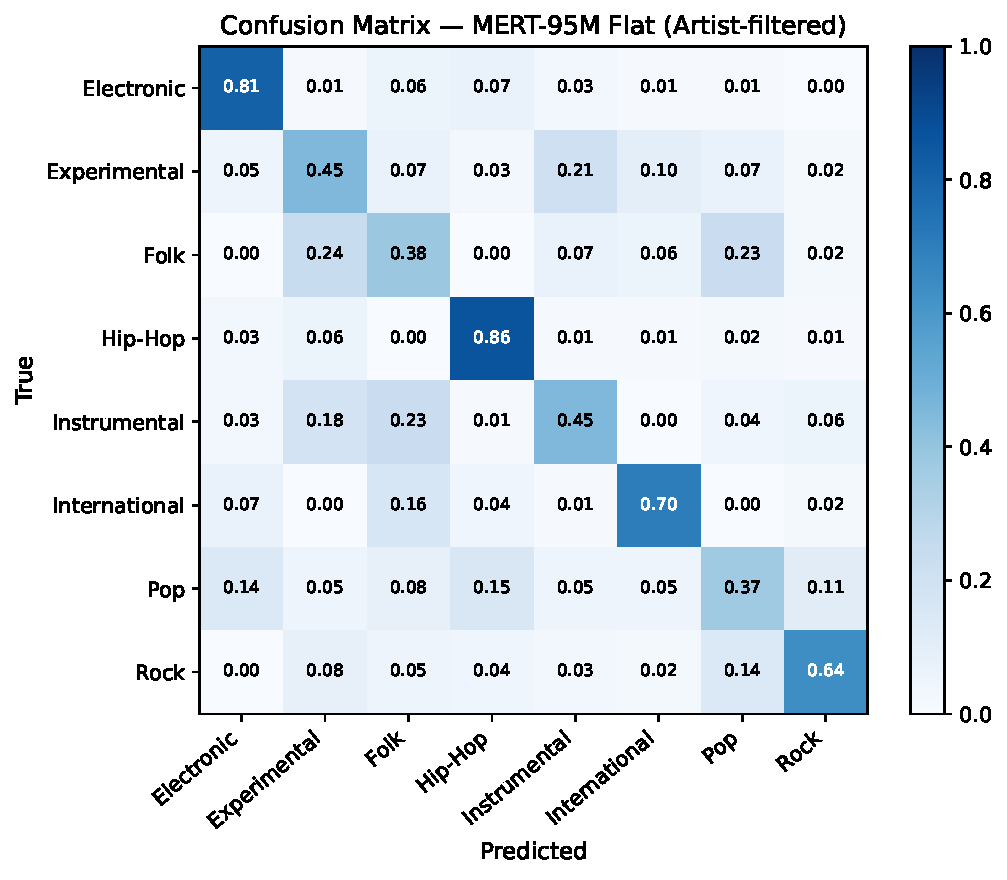
\includegraphics[width=\columnwidth]{confusion_best_artist_filtered.pdf}
\caption{Confusion matrix for MERT-95M flat probe (58.2\%) under the artist-filtered protocol. Hip-Hop (86/100) and Electronic (81/100) are well-separated; Folk (38/100) scatters into Experimental, Pop, and Instrumental.}
\label{fig:confusion_af}
\end{figure}

\begin{figure}[t]
\centering
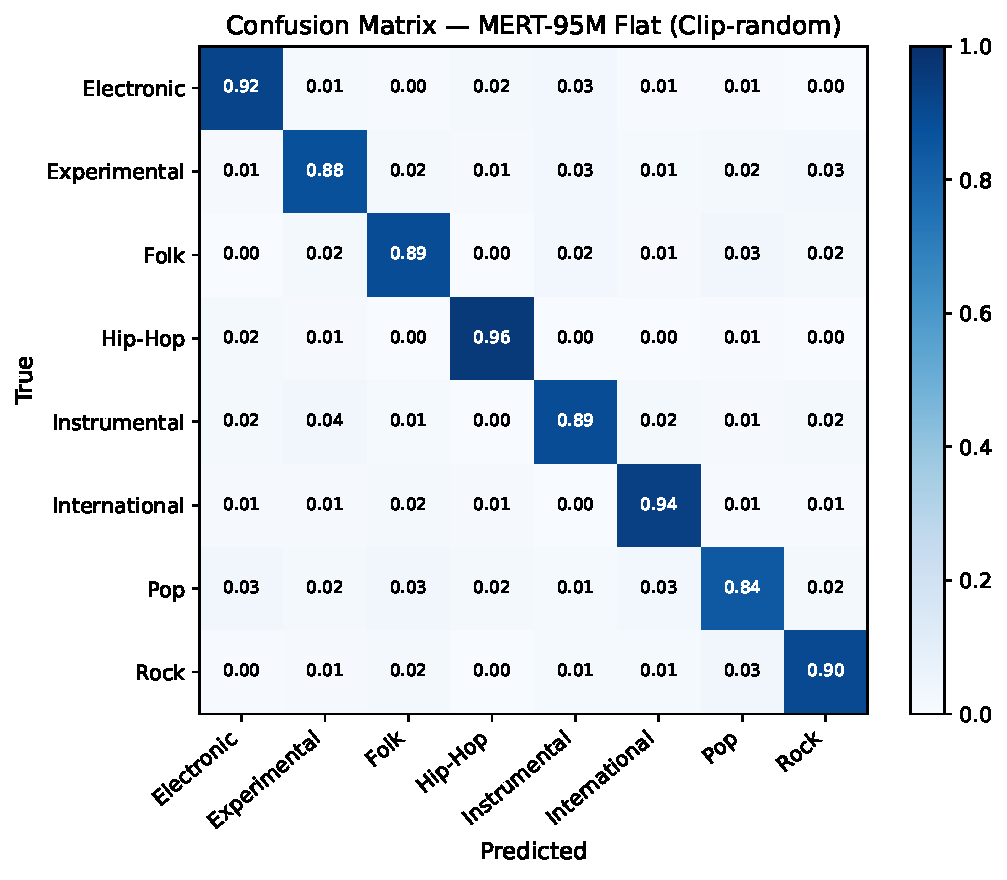
\includegraphics[width=\columnwidth]{confusion_best_cliprandom.pdf}
\caption{Confusion matrix for the \emph{same} model under clip-random evaluation (90.2\%). The diagonal dominates: every genre exceeds 530/630 correct. This is not improved classification --- it is the model recognising \emph{which recording} it has heard.}
\label{fig:confusion_cr}
\end{figure}

The architecture set confirms the fundamental finding: published
FMA-small results remain incomparable without protocol disclosure. The
inflation pattern holds across from-scratch CNNs, music-specific SSL
(MERT-95M, MERT-330M), general audio SSL (BYOL-A), supervised
pretraining (PANNs), audio-language models (CLAP), fine-tuned
transformers (AST, HTS-AT), and non-neural baselines (XGBoost).

\subsection{Fine-Tuning and DGX
Results}\label{g2.-fine-tuning-and-dgx-results}

The frozen-probing paradigm used in Sections A--G deliberately
restricts the backbone. We now report fine-tuning and multi-GPU probing
experiments conducted on an NVIDIA DGX cluster, testing whether
parameter adaptation closes the gap to permissive-protocol numbers.

\textbf{Round 1: Fine-tuned models.} Seven architectures were fine-tuned
under the artist-filtered protocol (Table IV, rows 38--44). The best
individual fine-tuned model is AST-Finetune at 58.1\%, which freezes
layers 0--6 of the AudioSet-pretrained AST and trains the classifier
head. It converged at epoch 1, suggesting strong feature alignment from
AudioSet pretraining. MERT-LoRA-330M (54.4\%, 2M trainable LoRA
parameters) underperformed the laptop frozen MERT-330M probe (56.6\%),
suggesting that LoRA adaptation struggles on the 6,400-track regime.
MERT-Unfreeze-330M (53.4\%, top 4 layers unfrozen with layer-wise LR
decay) fares even worse. Multi-crop inference (MERT-MultiCrop-330M,
53.9\%) adds nothing over standard LoRA (54.4\%). HTS-AT trained from
scratch reaches only 47.4\%, confirming the data-limited setting. Round
1 ensembles: a 4-model subset reaches 58.9\% and the full 7-model
uniform average reaches 58.5\% --- diminishing returns from adding
weaker models.

\textbf{Round 2: Probes on new backbones.} Layer-weighted MLP probes
trained on DGX with frozen embeddings from AST-AudioSet,
Whisper-Large-v3, MERT-330M, and CLAP (Table IV, rows 45--50). The AST
Probe reaches 62.0\%, becoming the new best single model --- 2.1 pp
above the laptop CLAP probe (59.9\%). The Fusion Probe (concatenation of
all four DGX encoder outputs) reaches 60.3\%. Whisper Probe and
MERT-330M Probe (DGX) reach 57.3\% and 57.9\% respectively. The DGX CLAP
Probe reaches only 27.8\%, sharply below the laptop CLAP probe (59.9\%);
this discrepancy reflects differences in the extraction pipeline (sample
rate, segment length, and CLAP model variant) and warrants further
investigation.

\textbf{Round 2 ensembles.} Caruana forward selection with replacement
\citep{kittler1998combining} produces a greedy ensemble at 61.8\%
(weights: AST-V2 28\%, Whisper 24\%, AST Probe 20\%, Fusion 12\%, MERT
12\%, CLAP 4\%). A simple uniform average of all six Round 2 models
reaches 62.1\% --- once again, uniform averaging beats learned
selection. This extends the pattern from Section E: at this data scale,
any learned combiner overfits.

\textbf{Validation--test gap.} Round 2 models show a 5--6 pp gap
between validation and test accuracy (e.g., AST Probe: 67.8\% val,
62.0\% test). This is larger than the 2--3 pp gap observed in laptop
probes and may reflect the smaller validation partition or systematic
distributional differences between the validation and test sets within
the artist-filtered split.

\textbf{Synthesis.} The frozen AST Probe (62.0\%) outperforms the
fine-tuned AST (58.1\%) on the same backbone. LoRA and partial
unfreezing on MERT do not beat a frozen probe. These results reinforce
the negative-result pattern of Section F: at FMA-small scale, the
accuracy ceiling is set by the backbone\textquotesingle s pretrained
representation quality and the evaluation protocol, not by the
adaptation method. Crucially, even the best DGX result (62.1\%) remains
far below the 90--96\% numbers achievable under permissive protocols,
confirming that the protocol --- not model capacity --- is the
dominant variable.

\subsection{Calibration Across
Protocols}\label{h.-calibration-across-protocols}

A model may achieve high accuracy under a permissive protocol, but does
it \emph{know} it is right? We measure Expected Calibration Error (ECE,
15 equal-width bins on {[}0, 1{]}), Brier score, and optimal temperature
across all 49 runs with cached episode outputs, grouped by protocol.

\begin{table}[t]
\centering
\caption{Calibration Metrics by Evaluation Protocol (Mean $\pm$ SD)}
\label{tab:calibration}
\footnotesize
\begin{tabular}{lcccc}
\toprule
\textbf{Protocol} & \textbf{ECE} & \textbf{Brier} & \textbf{Overconf.} & \textbf{$T^*$} \\
\midrule
Artist-filtered (27) & .060$\pm$.016 & .587$\pm$.012 & +0.5\,pp & 1.19$\pm$0.18 \\
Random-track (11)    & .067$\pm$.029 & .431$\pm$.030 & $-$4.7\,pp & 1.15$\pm$0.25 \\
Clip-random (11)     & .085$\pm$.045 & .186$\pm$.120 & $-$8.4\,pp & 0.76$\pm$0.14 \\
\bottomrule
\end{tabular}
\end{table}

\begin{figure}[t]
\centering
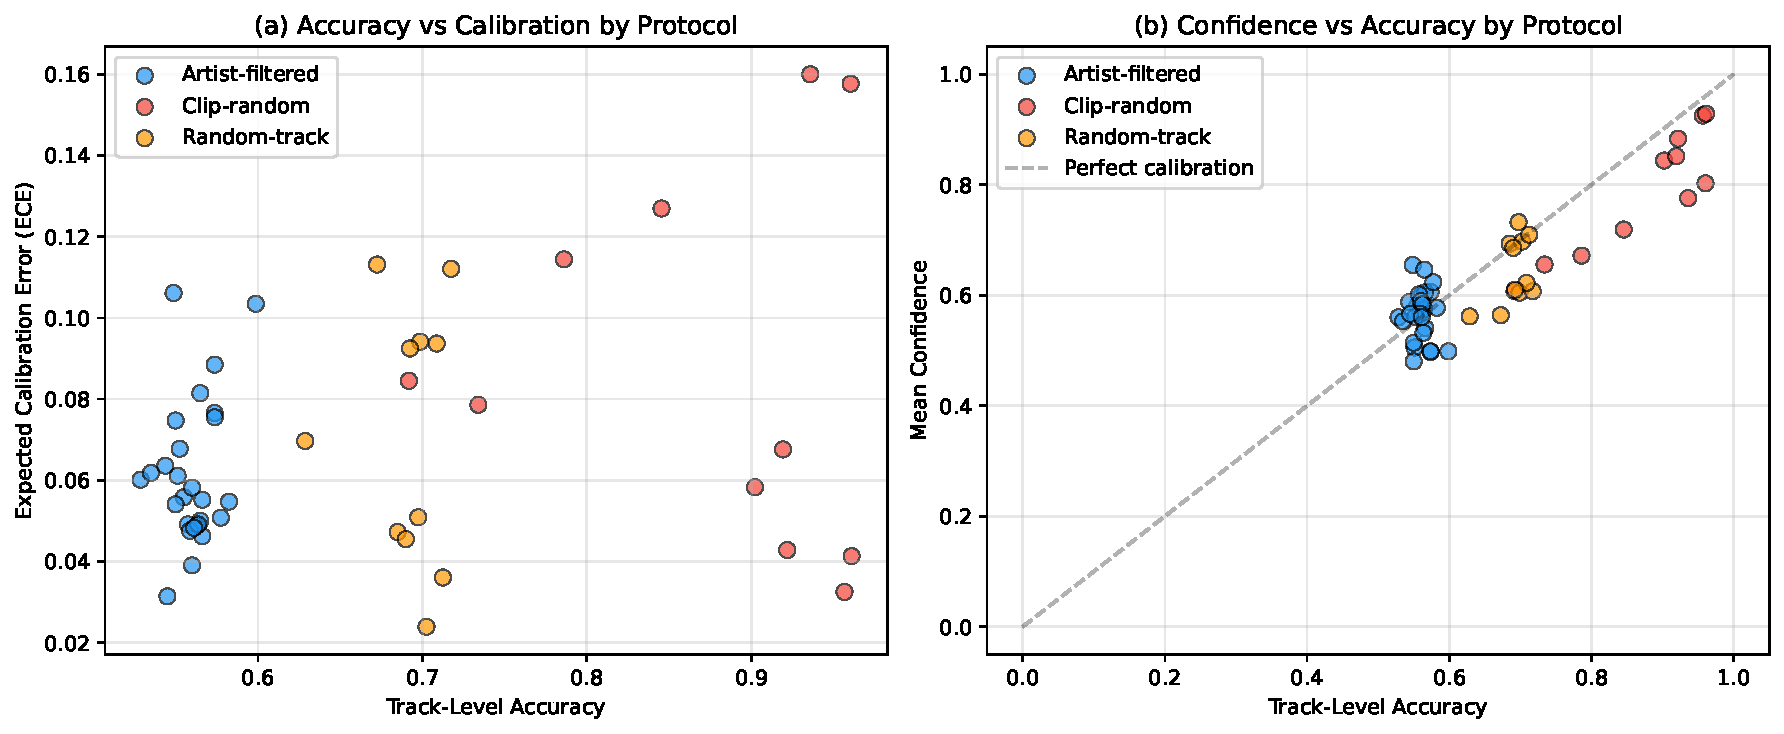
\includegraphics[width=\columnwidth]{calibration_by_protocol.pdf}
\caption{Calibration comparison across evaluation protocols. Under the artist-filtered protocol, models are roughly calibrated (overconfidence $\approx$ +0.9~pp). Under clip-random evaluation, all 10 models are \emph{underconfident}: their inflated accuracy outpaces the softmax probabilities. Temperature scaling with $T^* < 1$ is needed to sharpen predictions to match the inflated accuracy.}
\label{fig:calibration}
\end{figure}

\begin{figure}[t]
\centering
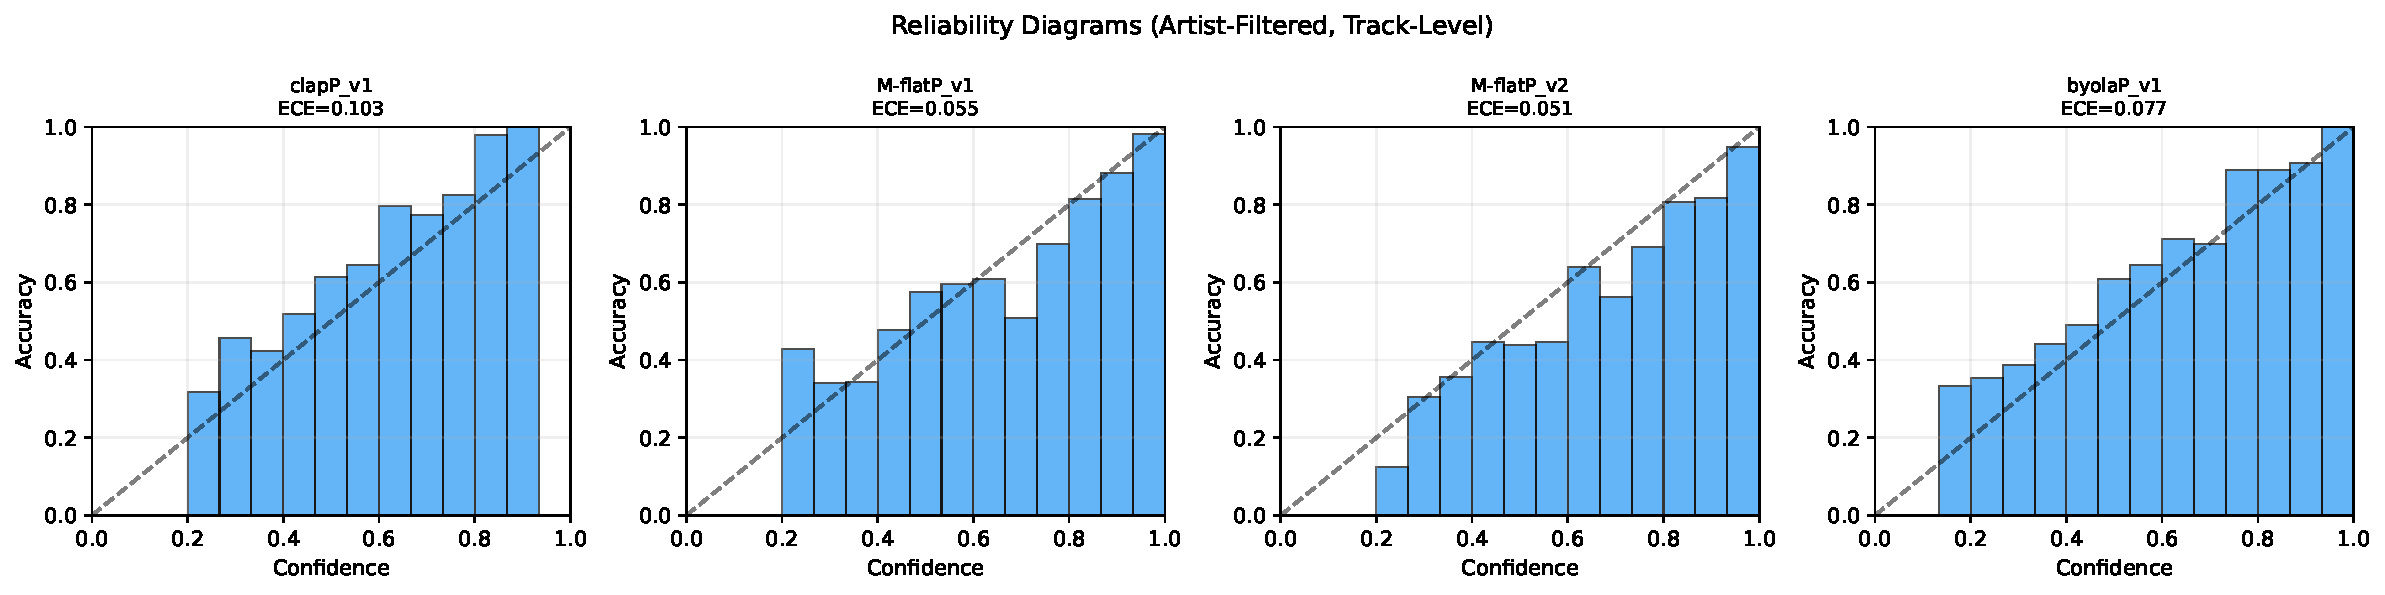
\includegraphics[width=\columnwidth]{reliability_diagrams.pdf}
\caption{Reliability diagrams for representative models under each protocol. Under honest evaluation, the calibration curve tracks the diagonal. Under clip-random evaluation, the curve falls below the diagonal across all confidence bins --- the model is less confident than it is accurate.}
\label{fig:reliability}
\end{figure}

Table \ref{tab:calibration} and Figures
\ref{fig:calibration}--\ref{fig:reliability} reveal a counterintuitive
finding: \textbf{leakage creates underconfidence, not overconfidence.}
Under the artist-filtered protocol, models are approximately calibrated
(mean overconfidence +0.5 pp). Under clip-random evaluation, all 11
models are underconfident (mean \$-\$8.4 pp): the inflated accuracy
exceeds the model\textquotesingle s own confidence. This happens because
the softmax probabilities are calibrated to the difficulty of the genre
classification task, but the permissive protocol converts the task from
genre classification to recording recognition --- which the model
solves correctly more often than its softmax entropy suggests.

Temperature scaling confirms this: artist-filtered models need
\(T^* > 1\) (softening, reducing overconfidence), while clip-random
models need \(T^* < 1\) (sharpening, increasing confidence to match
inflated accuracy). The optimal temperature is itself a diagnostic for
protocol leakage: \(T^* \ll 1\) signals that the model achieves accuracy
it did not learn to expect.

\subsection{Representation Similarity
(CKA)}\label{i.-representation-similarity-cka}

To understand whether backbone diversity drives ensemble gain, we
compute linear Centered Kernel Alignment (CKA)
\citep{kornblith2019similarity} between the mean-pooled test-set
representations of all five backbone families (800 tracks, aligned by
track ID).

\begin{figure*}[t]
\centering
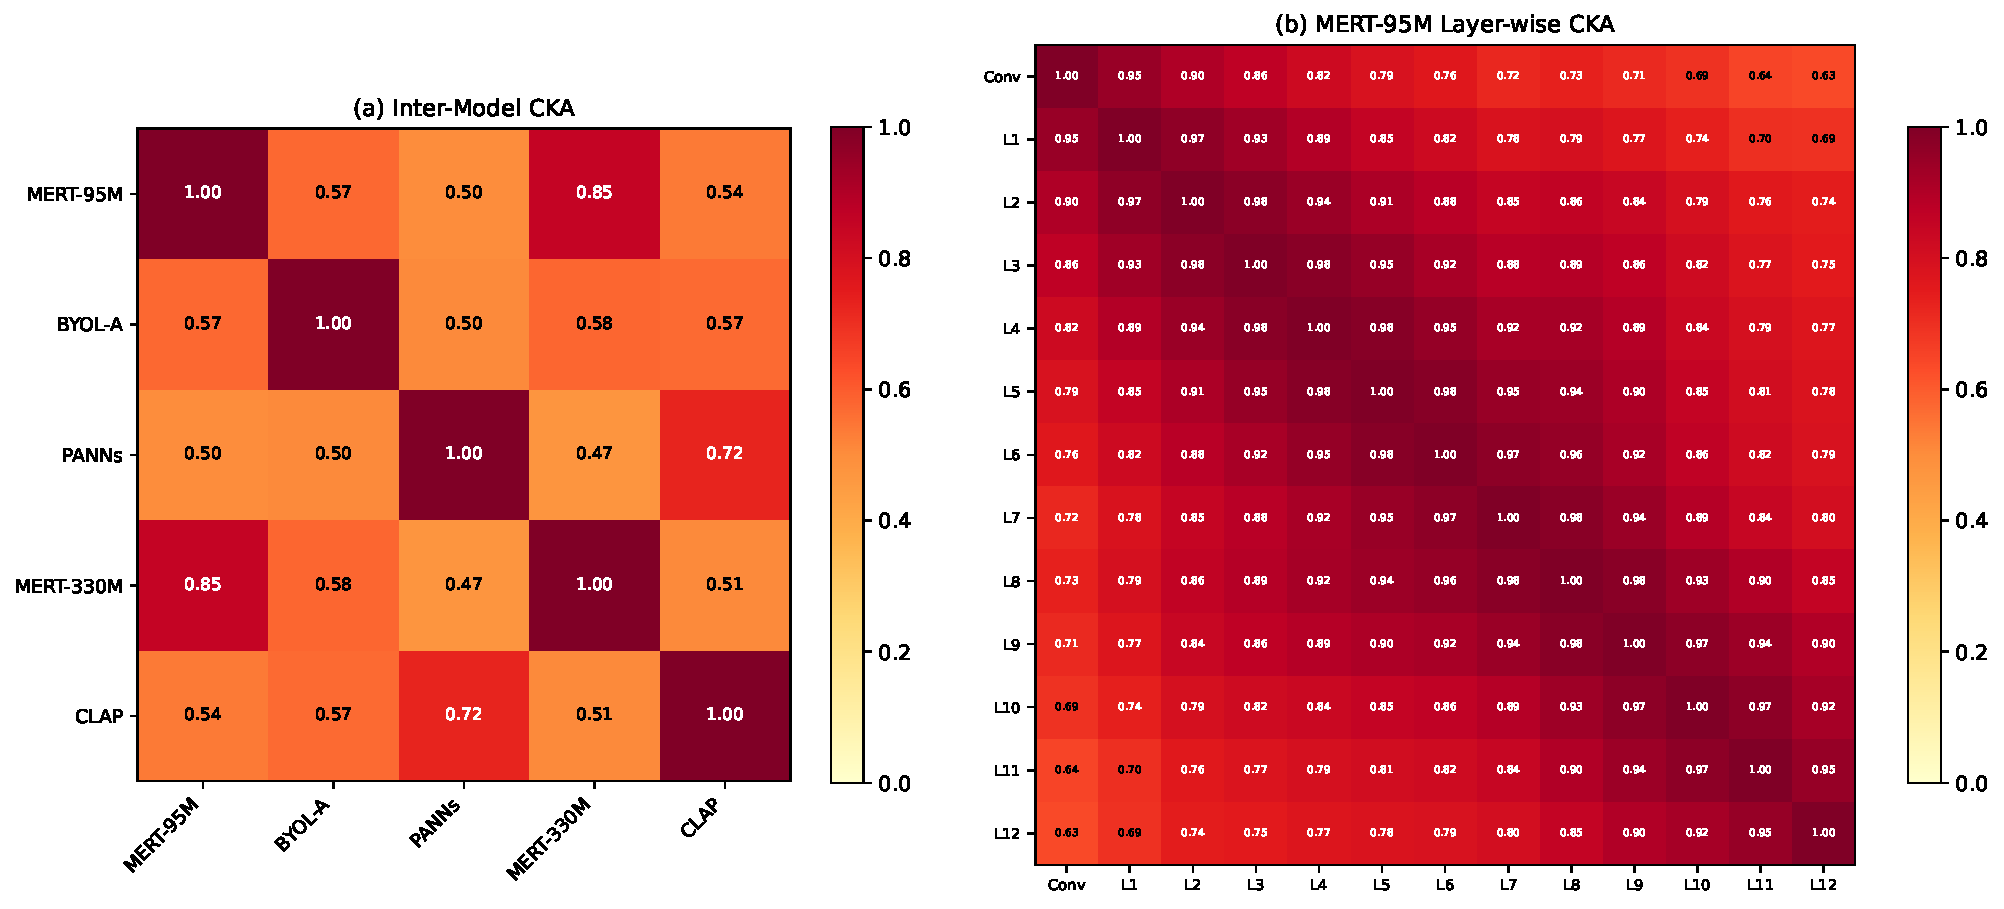
\includegraphics[width=\textwidth]{cka_combined.pdf}
\caption{(a) Inter-model CKA across 5 backbones: MERT-95M and MERT-330M share a high CKA (0.848); CLAP and PANNs show surprising similarity (0.724), likely reflecting their shared AudioSet-scale pretraining. (b) MERT-95M layer-wise CKA: adjacent layers are highly similar ($\geq$ 0.94), with a gradual phase transition around layer 8--9 where representations shift from acoustic to semantic.}
\label{fig:cka}
\end{figure*}

The inter-model CKA matrix (Figure \ref{fig:cka}) reveals that MERT-95M
and MERT-330M encode nearly identical information (CKA = 0.848),
explaining why MERT-330M does not outperform MERT-95M under honest
evaluation: the larger model\textquotesingle s additional capacity does
not add complementary features. CLAP and PANNs show surprisingly high
similarity (CKA = 0.724), likely because both encode broad acoustic
categories --- PANNs via supervised classification on
AudioSet\textquotesingle s 527 classes, CLAP via contrastive alignment
with audio-text pairs spanning a similar domain. BYOL-A occupies an
intermediate position, moderately similar to all backbones
(0.505--0.576).

The most diverse pair is PANNs \(\leftrightarrow\) MERT-330M (CKA =
0.469), followed by MERT-330M \(\leftrightarrow\) CLAP (0.507). This
diversity explains why a uniform ensemble over architecturally diverse
backbones outperforms any single model: the component models make
different errors because they encode different information.

Within MERT-95M, the \(13\times13\) layer-wise CKA heatmap shows a
smooth gradient from early to late layers, with adjacent layers highly
redundant (CKA \(\geq 0.94\)). A phase transition occurs around layers
8--9, where the CKA between early layers (0--4) and late layers
(10--12) drops below 0.80. This is consistent with the speech SSL
literature\textquotesingle s finding that early transformer layers
encode acoustic features while later layers encode more abstract,
task-relevant representations \citep{pasad2021layer}.

\subsection{Error Diversity and Ensemble
Complementarity}\label{j.-error-diversity-and-ensemble-complementarity}

We compute pairwise Cohen\textquotesingle s kappa and
Yule\textquotesingle s Q between the correctness vectors of 8
representative models (one best-per-architecture) to quantify error
diversity.

\begin{figure*}[t]
\centering
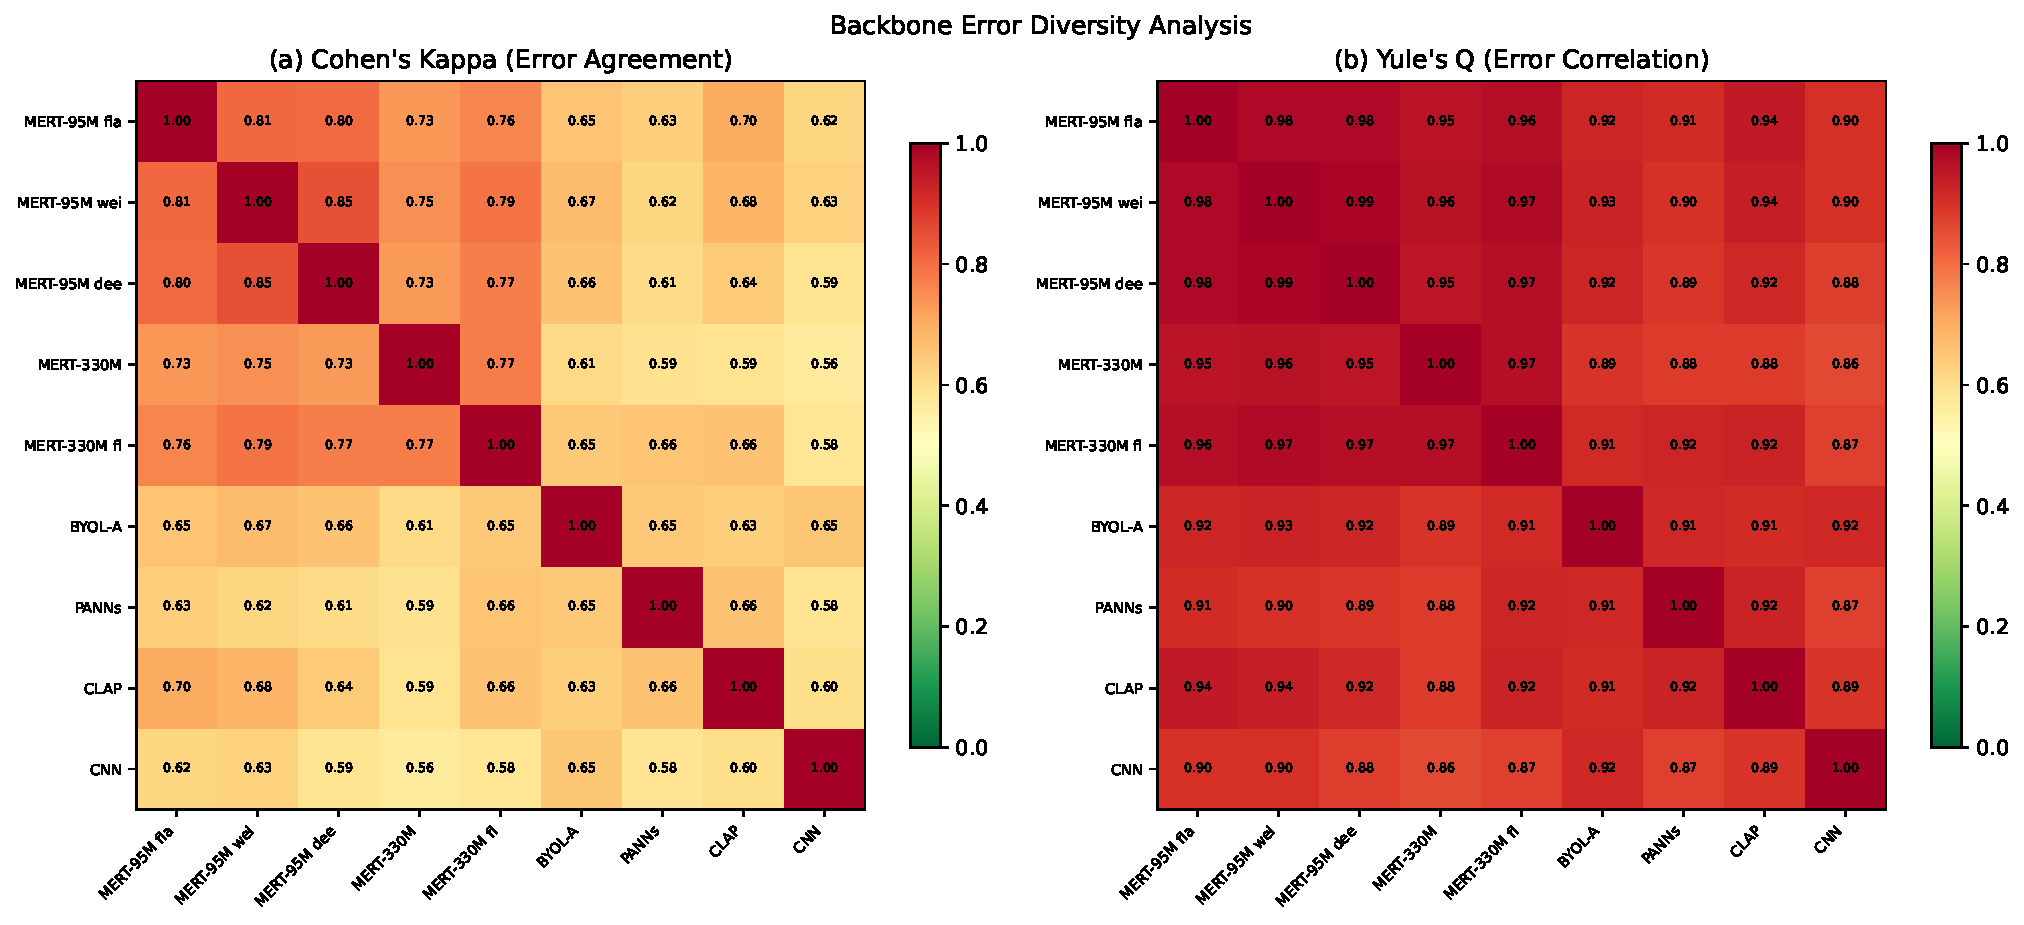
\includegraphics[width=\textwidth]{error_diversity_heatmap.pdf}
\caption{(a) Cohen's kappa measures agreement in correct/incorrect predictions. Within-MERT pairs agree strongly ($\kappa = 0.775 \pm 0.035$); cross-family pairs are more diverse ($\kappa = 0.630 \pm 0.034$). (b) Yule's Q confirms the same pattern with the error correlation measure.}
\label{fig:error_diversity}
\end{figure*}

The error diversity heatmap (Figure \ref{fig:error_diversity}) reveals
clear patterns. Within-MERT variants show high error agreement
(\(\kappa = 0.775 \pm 0.035\)): they share the same backbone, so the
same tracks tend to confuse them. Cross-family pairs are substantially
more diverse (\(\kappa = 0.630 \pm 0.034\)). The most diverse pairs
involve architecturally distinct backbones (CNN, PANNs, CLAP vs. MERT
variants), confirming that ensemble diversity requires crossing model
family boundaries.

Among the top 4 models, 216 tracks (27.0\%) are misclassified by all
four --- these represent a hard core of genuinely ambiguous tracks
that no single-backbone probe can solve. Another 337 tracks (42.1\%) are
correctly classified by all four. The remaining 247 tracks (30.9\%) are
where ensemble diversity provides value: at least one model gets it
right while others do not.

This quantifies why uniform ensembling works and learned fusion does
not. The models\textquotesingle{} errors are moderately correlated (mean
\(\kappa = 0.670\)) --- diverse enough for averaging to help, but
not diverse enough for a learned combiner to find exploitable patterns
at this data scale.

\subsection{Temporal Stability of Genre
Predictions}\label{k.-temporal-stability-of-genre-predictions}

Each 30-second FMA track yields 10 three-second episodes. We analyse how
consistently models classify episodes from the same track.

\begin{figure}[t]
\centering
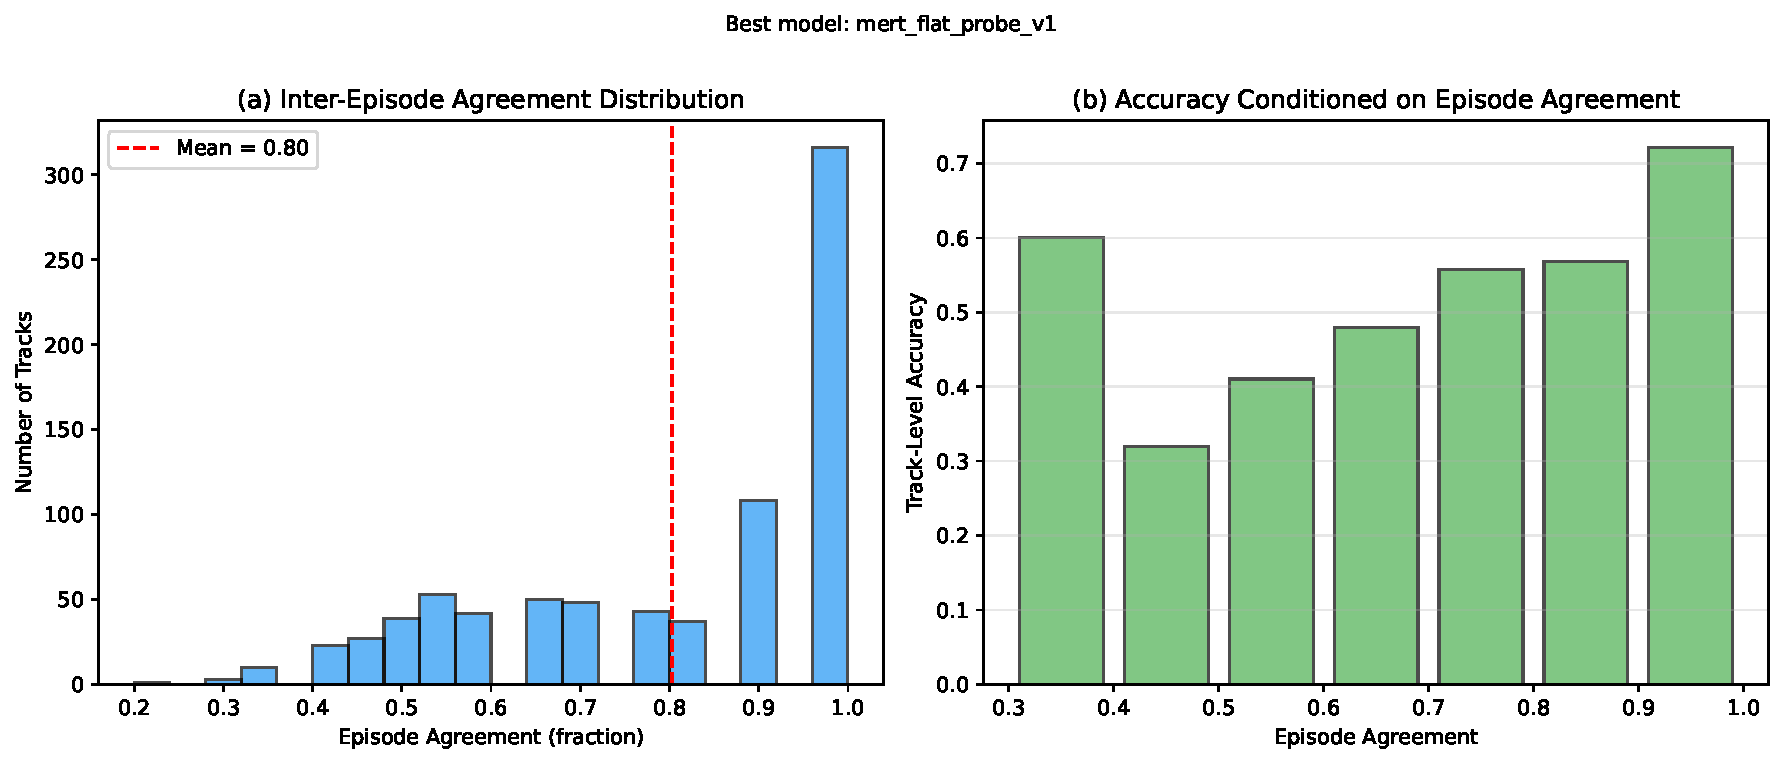
\includegraphics[width=\columnwidth]{episode_agreement.pdf}
\caption{(a) Distribution of inter-episode agreement (fraction of episodes per track that agree with the majority vote). 39.5\% of tracks achieve unanimous agreement across all 10 episodes. (b) Track-level accuracy conditioned on agreement: tracks with $\geq$ 90\% agreement reach 72.1\% accuracy; tracks with $<$ 50\% agreement drop to 35.9\%.}
\label{fig:agreement}
\end{figure}

\begin{figure}[t]
\centering
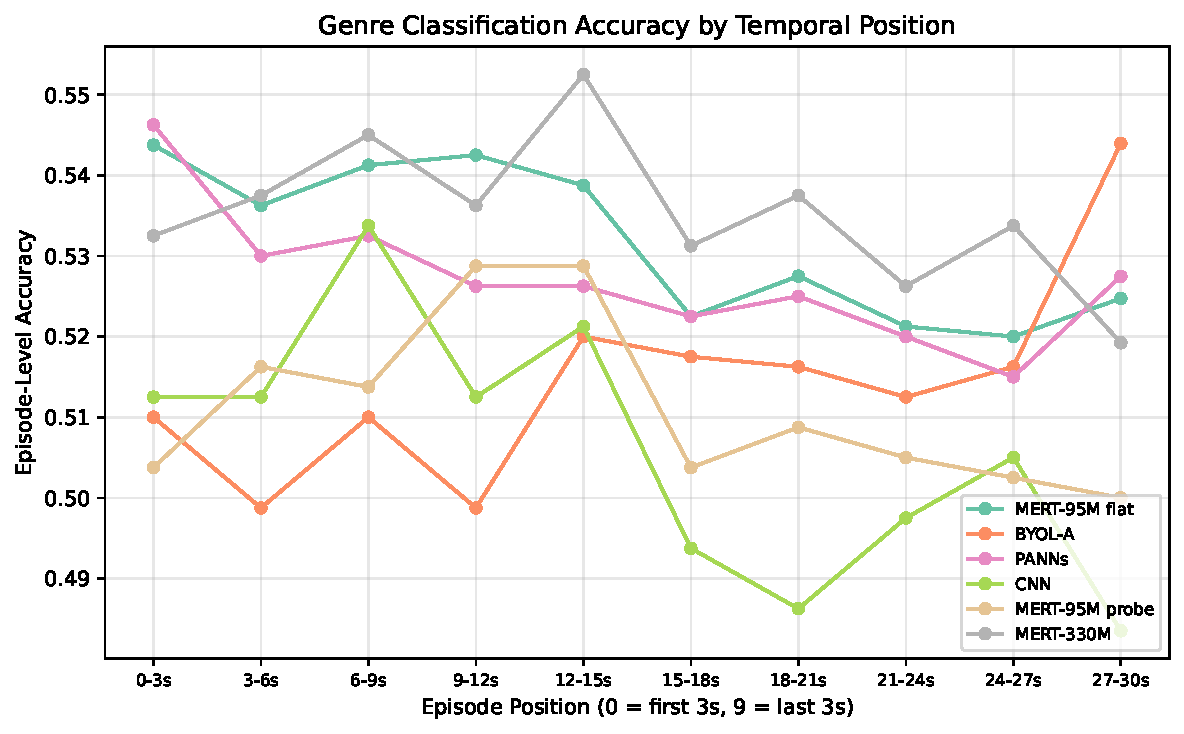
\includegraphics[width=\columnwidth]{temporal_accuracy.pdf}
\caption{Episode-level accuracy by temporal position for 6 representative models. Accuracy is roughly flat across positions 0--9 (first 3\,s to last 3\,s), with no model showing a consistent temporal trend. This suggests that genre-discriminative information is distributed throughout the track, not concentrated at the beginning or end.}
\label{fig:temporal}
\end{figure}

Figures \ref{fig:agreement} and \ref{fig:temporal} illustrate temporal
stability. Mean episode agreement is 80.3\% \(\pm\) 20.5\% ---
higher than chance but far from unanimous. Tracks with high agreement
(\(\geq\) 90\%) are classified with 72.1\% accuracy, while low-agreement
tracks (\(<\) 50\%) achieve only 35.9\%. This 36-pp gap shows that
inter-episode agreement is a strong confidence signal: a model that is
consistent across temporal positions is more likely to be correct.

Per-genre agreement varies systematically: Hip-Hop (87.5\%) and
International (88.6\%) achieve the highest temporal consistency, while
Folk (71.6\%) and Pop (70.6\%) are the most temporally variable. The
same genres that are hardest to classify are also hardest to classify
\emph{consistently} --- suggesting that the difficulty is not in any
particular 3-second segment but in the genre\textquotesingle s intrinsic
acoustic diffuseness.

Accuracy is roughly flat across episode positions (range:
52.0\%--54.4\% for the best model), with no model showing a consistent
improvement or degradation from the beginning to the end of a track.
This flatness suggests that 3-second episodes are individually
informative regardless of their position, and that the track-level
aggregation we use (mean-pooling softmax probabilities) is not
systematically harmed by any particular temporal position.

\subsection{Statistical Rigour}\label{l.-statistical-rigour}

All accuracy numbers in this study are accompanied by bootstrap 95\%
confidence intervals (10,000 resamples, percentile method, resampled at
the track level to respect hierarchical structure; \(n = 800\) test
tracks). The best laptop model (CLAP probe, 59.9\%) has CI {[}56.5\%,
63.1\%{]}. McNemar\textquotesingle s chi-squared test between all pairs
of the top 8 artist-filtered models finds no significant difference
after multiple-comparison correction (Bonferroni-corrected threshold
\(\alpha = 0.05/28 = 0.0018\); all 28 individual \(p\)-values exceed
this threshold, with only 2 pairs falling below the uncorrected
\(\alpha = 0.05\)): the top cluster of models is statistically
indistinguishable.

\begin{figure}[t]
\centering
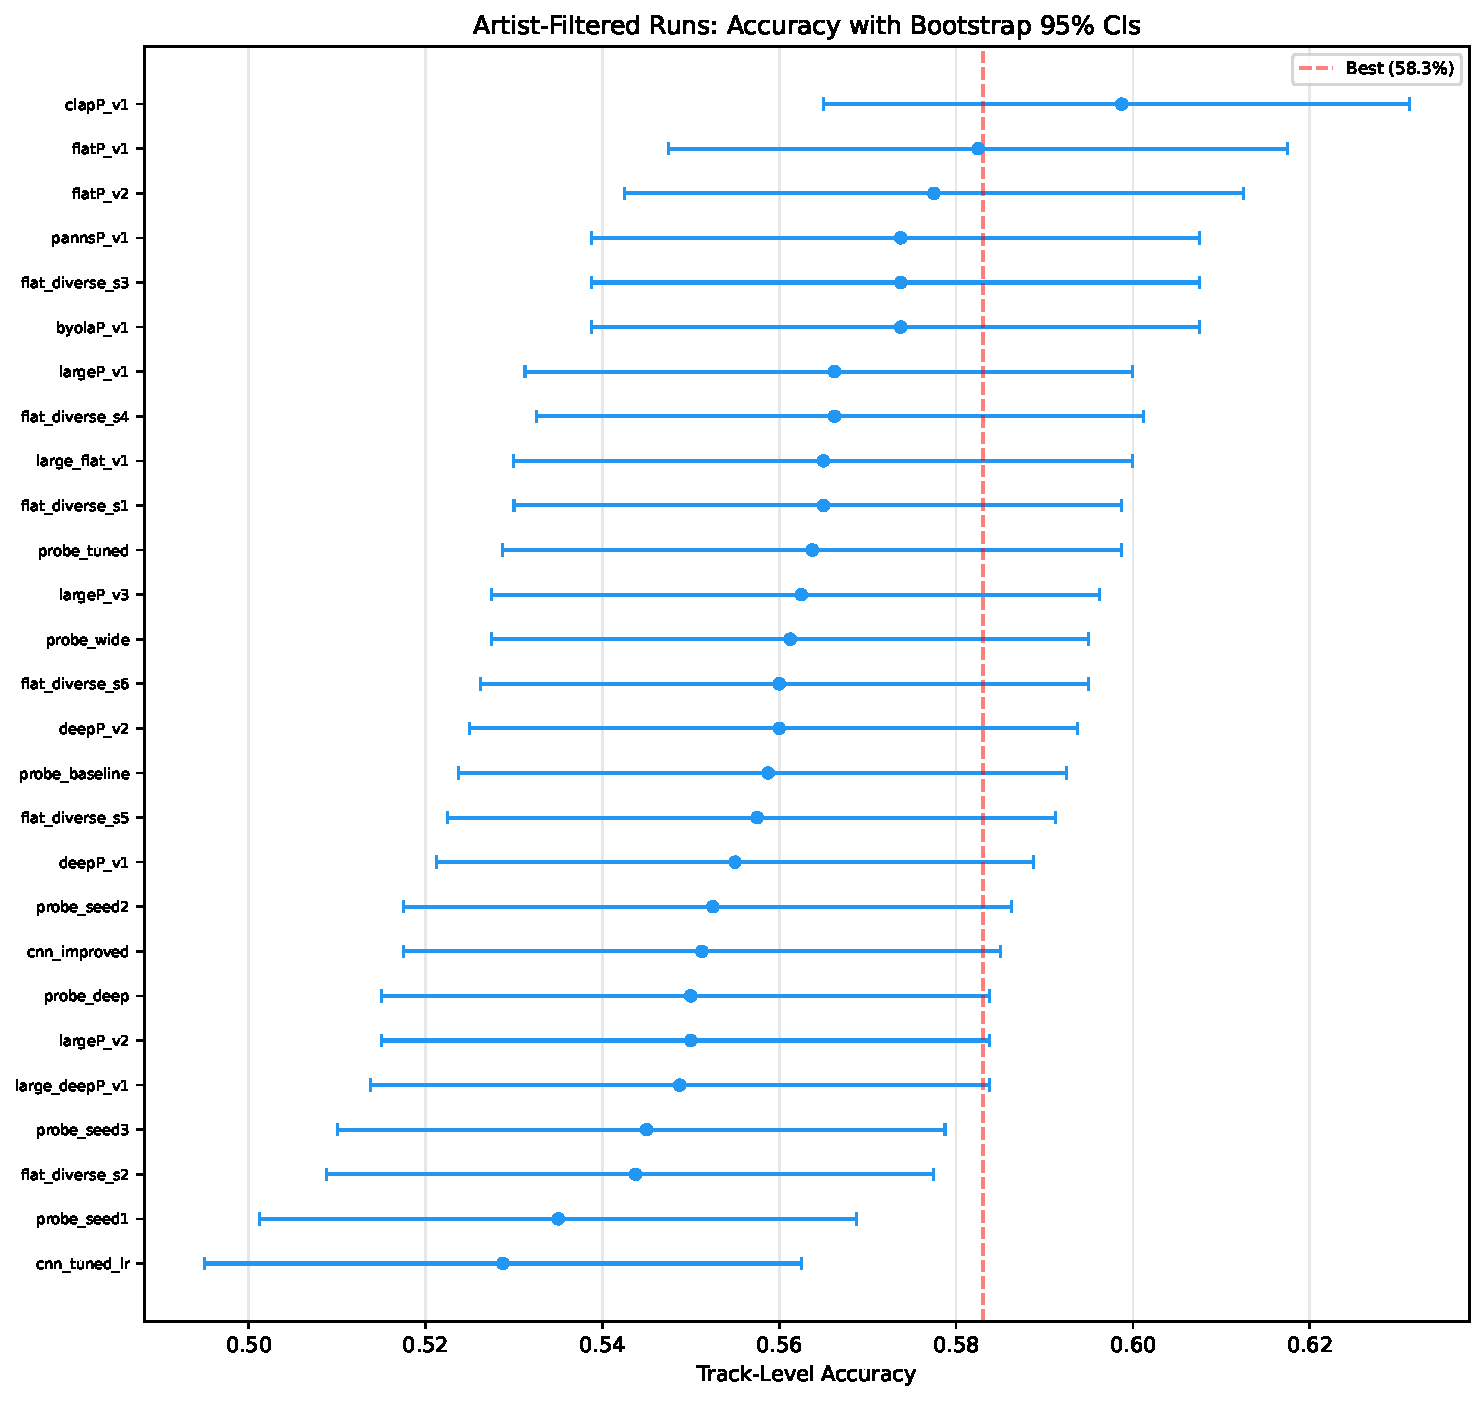
\includegraphics[width=\columnwidth]{bootstrap_forest.pdf}
\caption{Bootstrap 95\% confidence intervals for all 26 artist-filtered runs. The top cluster (7 runs above 56\%) has widely overlapping CIs, confirming that differences within the cluster are not statistically significant.}
\label{fig:forest}
\end{figure}

The forest plot (Figure \ref{fig:forest}) confirms the overlapping CIs.
Per-genre CIs for the best model reveal the precision ceiling: Hip-Hop
has the tightest CI {[}79.0\%, 92.0\%{]}, while the hardest genres have
wide CIs (Folk: {[}28.0\%, 47.0\%{]}, Pop: {[}28.0\%, 47.0\%{]}). With
only 100 test tracks per genre, detecting a 5-pp improvement in Folk
with 95\% confidence would require a model to improve from 38\% to 43\%
--- a bar that is meaningful but attainable.

\subsection{Layer-Wise Leakage
Fingerprinting}\label{m.-layer-wise-leakage-fingerprinting}

\begin{figure*}[t]
\centering
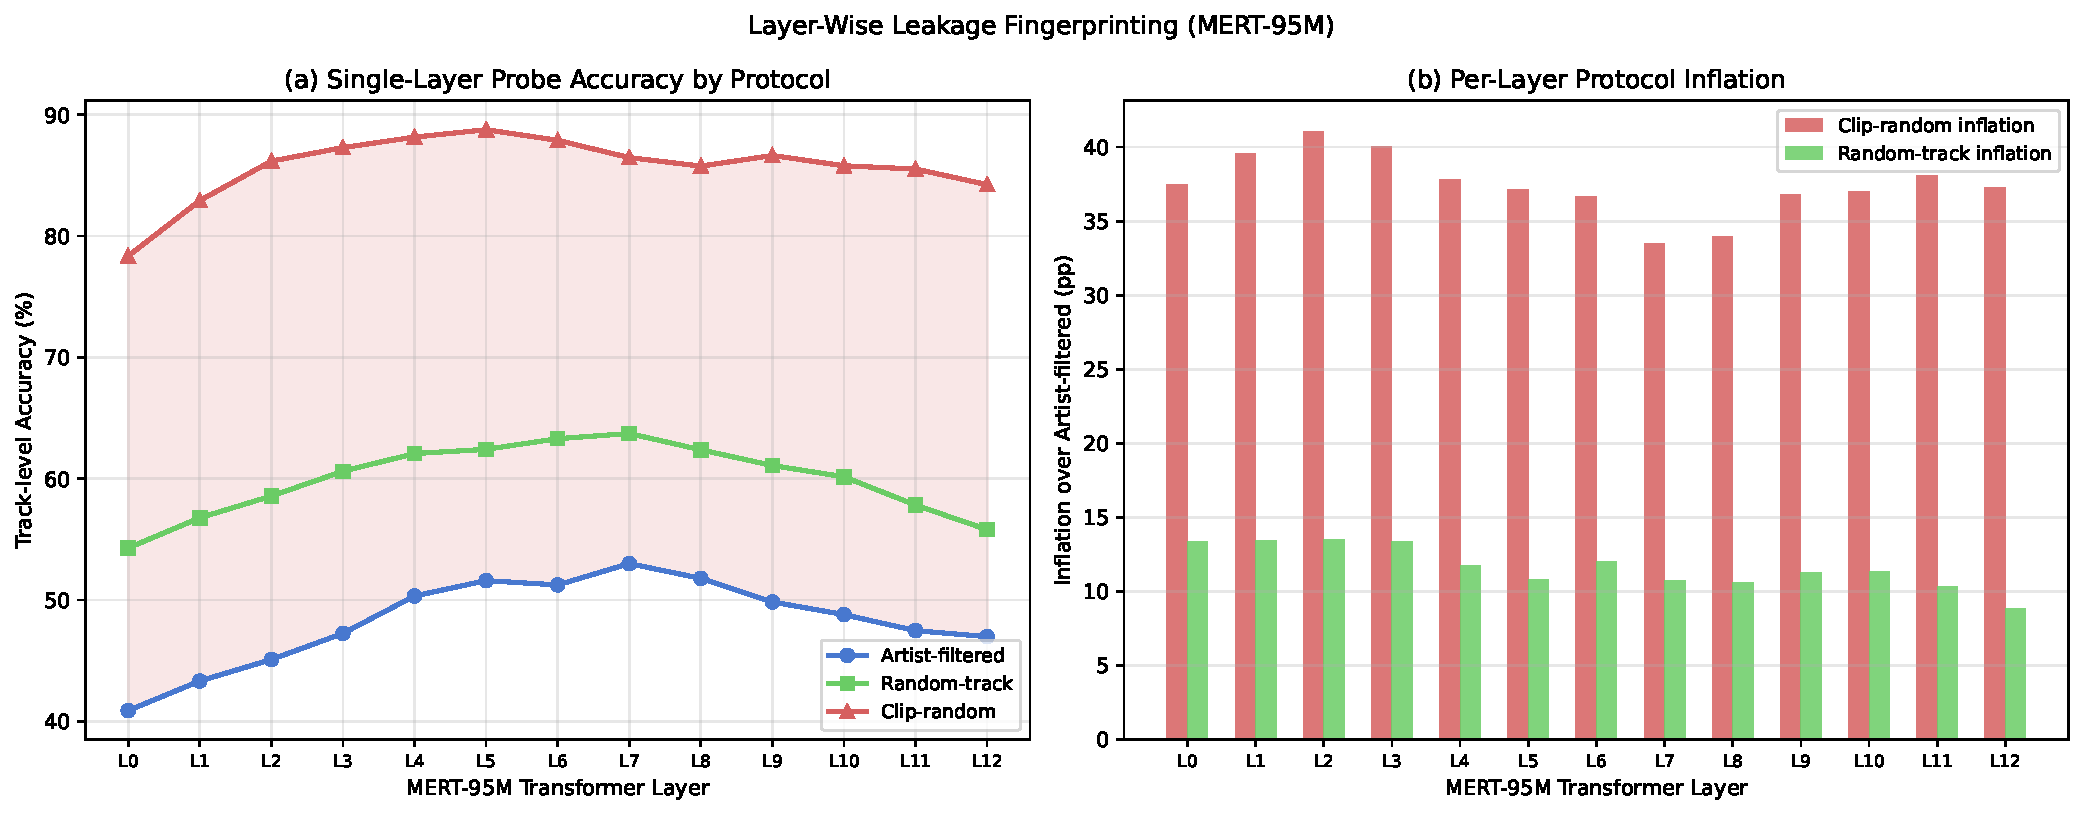
\includegraphics[width=\textwidth]{layer_leakage.pdf}
\caption{(a) Single-layer MERT-95M probe accuracy under three protocols. Genre-discriminative accuracy (blue) peaks at layer~7 (53.0\%) and declines in later layers. Clip-random accuracy (red) peaks at layers~3--5 (87--89\%) and remains high across all depths. The shaded region shows the inflation gap. (b) Per-layer inflation. Despite the inverted-U shape in honest accuracy, inflation is remarkably uniform (33.5--41.1~pp across all 13 layers), indicating that recording identity is encoded at every transformer depth, not just in early acoustic layers.}
\label{fig:layer_leakage}
\end{figure*}

To localise where recording identity versus genre information resides in
a pretrained transformer (Figure \ref{fig:layer_leakage}), we train 13
single-layer MERT-95M probes --- one per transformer layer ---
under each of the three protocols (39 runs total).

Genre-discriminative accuracy follows an inverted-U pattern: it rises
from layer\textasciitilde0 (40.9\%) through layer\textasciitilde7
(53.0\%), then declines to layer\textasciitilde12 (47.0\%). This pattern
is consistent with prior findings that genre-relevant features are
distributed across transformer depth, with middle layers encoding the
richest semantic representations.

The key finding is that inflation is \emph{nearly uniform} across
layers: it ranges from +33.5\textasciitilde pp (layer\textasciitilde7)
to +41.1\textasciitilde pp (layer\textasciitilde2), with a mean of
+37.4\textasciitilde pp. If recording identity were concentrated in
early acoustic layers (which preserve fine-grained spectral detail), we
would expect inflation to decay with depth. Instead, the uniformity
indicates that recording identity pervades the entire representation
--- the model encodes enough recording-specific information at every
layer for a simple probe to exploit it under permissive evaluation.

The slight inflation minimum at layer\textasciitilde7 --- the same
layer with peak honest accuracy --- suggests a subtle tradeoff: the
layer most useful for genre classification is also the layer that
encodes proportionally more genre (vs. recording) information. But the
effect is small: even at layer\textasciitilde7, inflation is
+33.5\textasciitilde pp, indicating that recording identity dominates
genre information at every depth.

\subsection{Data Efficiency and Protocol
Sensitivity}\label{n.-data-efficiency-and-protocol-sensitivity}

\begin{figure*}[t]
\centering
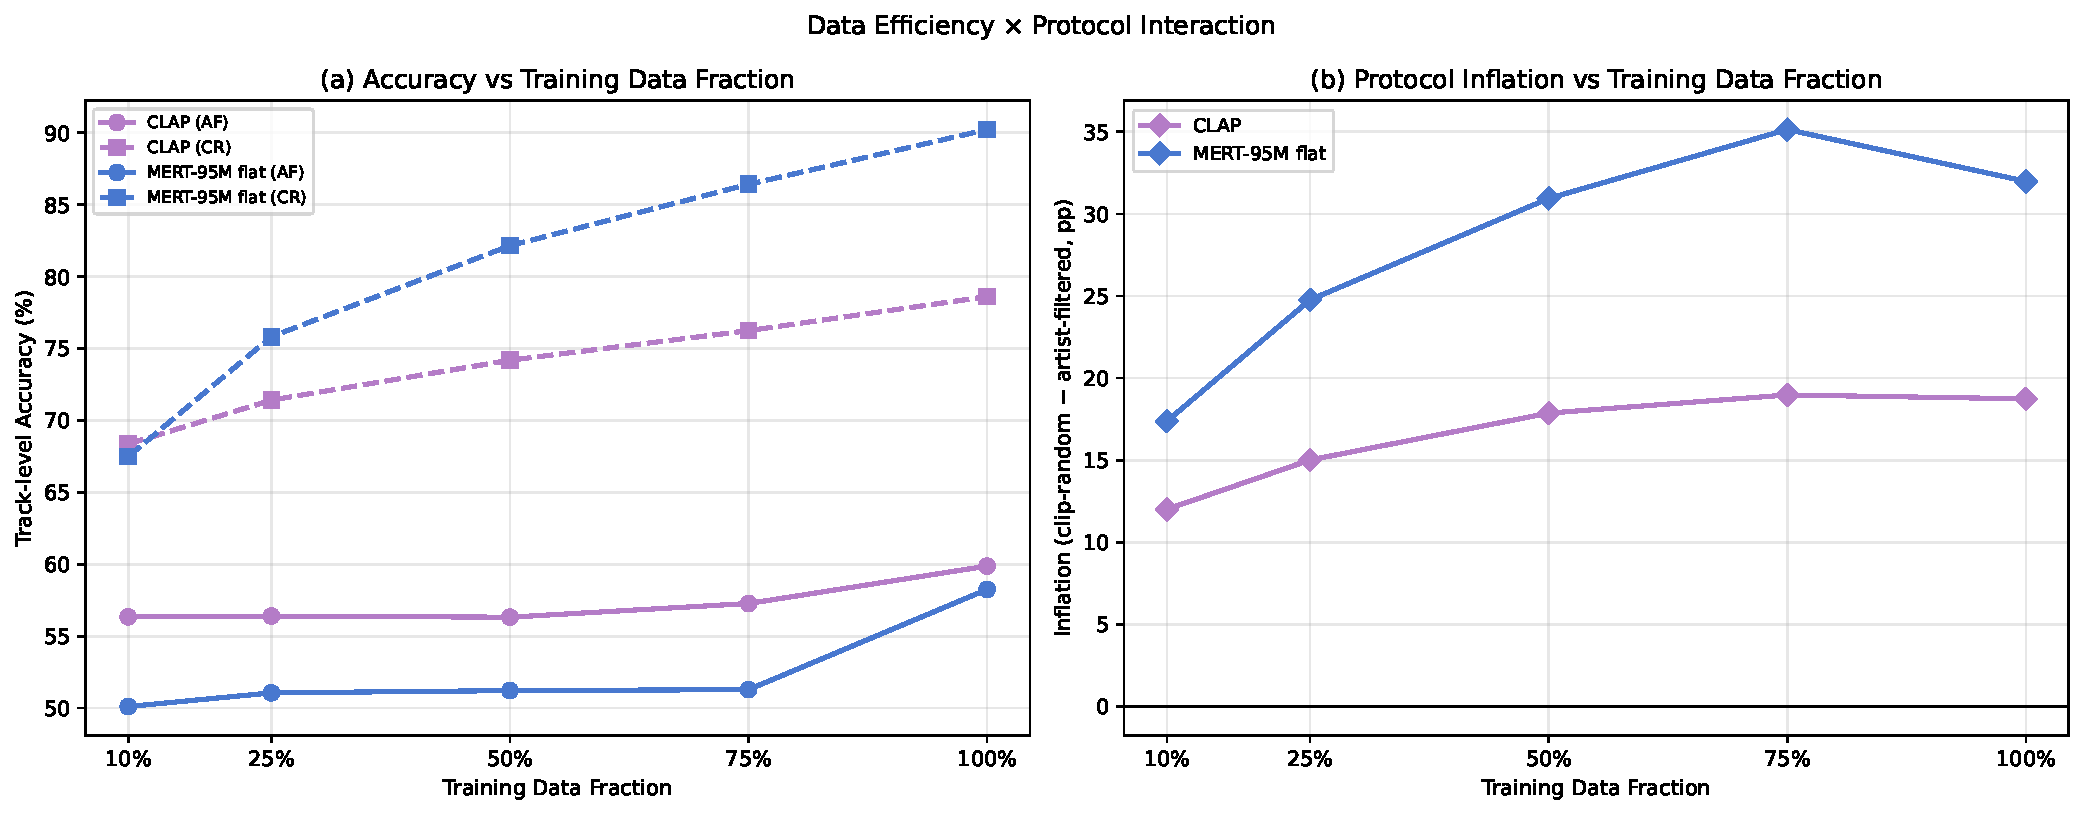
\includegraphics[width=\textwidth]{data_efficiency.pdf}
\caption{(a) Track-level accuracy vs training data fraction for CLAP and MERT-95M flat probes under artist-filtered (solid) and clip-random (dashed) evaluation. Under honest evaluation, both models plateau early; under leakage, accuracy scales steadily with data. (b) Inflation (clip-random $-$ artist-filtered) vs training data fraction. Inflation grows monotonically with training set size: MERT flat inflates from +17.4~pp at 10\% to +35.1~pp at 75\%; CLAP inflates from +12.0~pp to +19.0~pp. More training data means more recordings to memorise, amplifying the leakage effect.}
\label{fig:data_efficiency}
\end{figure*}

To test whether leakage is a small-data artifact (Figure
\ref{fig:data_efficiency}), we train CLAP and MERT-95M flat probes on
subsampled training sets (10\%, 25\%, 50\%, 75\%, 100\%) under both
artist-filtered and clip-random evaluation.

Under honest evaluation, accuracy is remarkably insensitive to training
set size: CLAP ranges from 56.3\% (10\% data) to 59.9\% (100\%), and
MERT flat from 50.1\% to 58.2\%. The frozen representations already
contain the genre information; more labelled data provides diminishing
returns for learning the linear mapping.

Under clip-random evaluation, accuracy scales steeply: MERT flat rises
from 67.5\% (10\%) to 90.2\% (100\%). The inflation consequently grows
monotonically: from +17.4\textasciitilde pp at 10\% to
+35.1\textasciitilde pp at 75\% for MERT flat, and from
+12.0\textasciitilde pp to +19.0\textasciitilde pp for CLAP. This
scaling confirms that leakage is not a small-data artifact --- it is
a memorisation effect that strengthens as the model sees more
recordings. The practical implication is sobering: growing a benchmark
dataset does not mitigate protocol leakage; it amplifies it.

\subsection{Temporal Consistency as a Protocol
Diagnostic}\label{o.-temporal-consistency-as-a-protocol-diagnostic}

Section 5K showed that inter-episode agreement under honest evaluation
averages 80.3\%. We now compare this to agreement under clip-random
evaluation across 8 paired architectures.

\begin{figure*}[t]
\centering
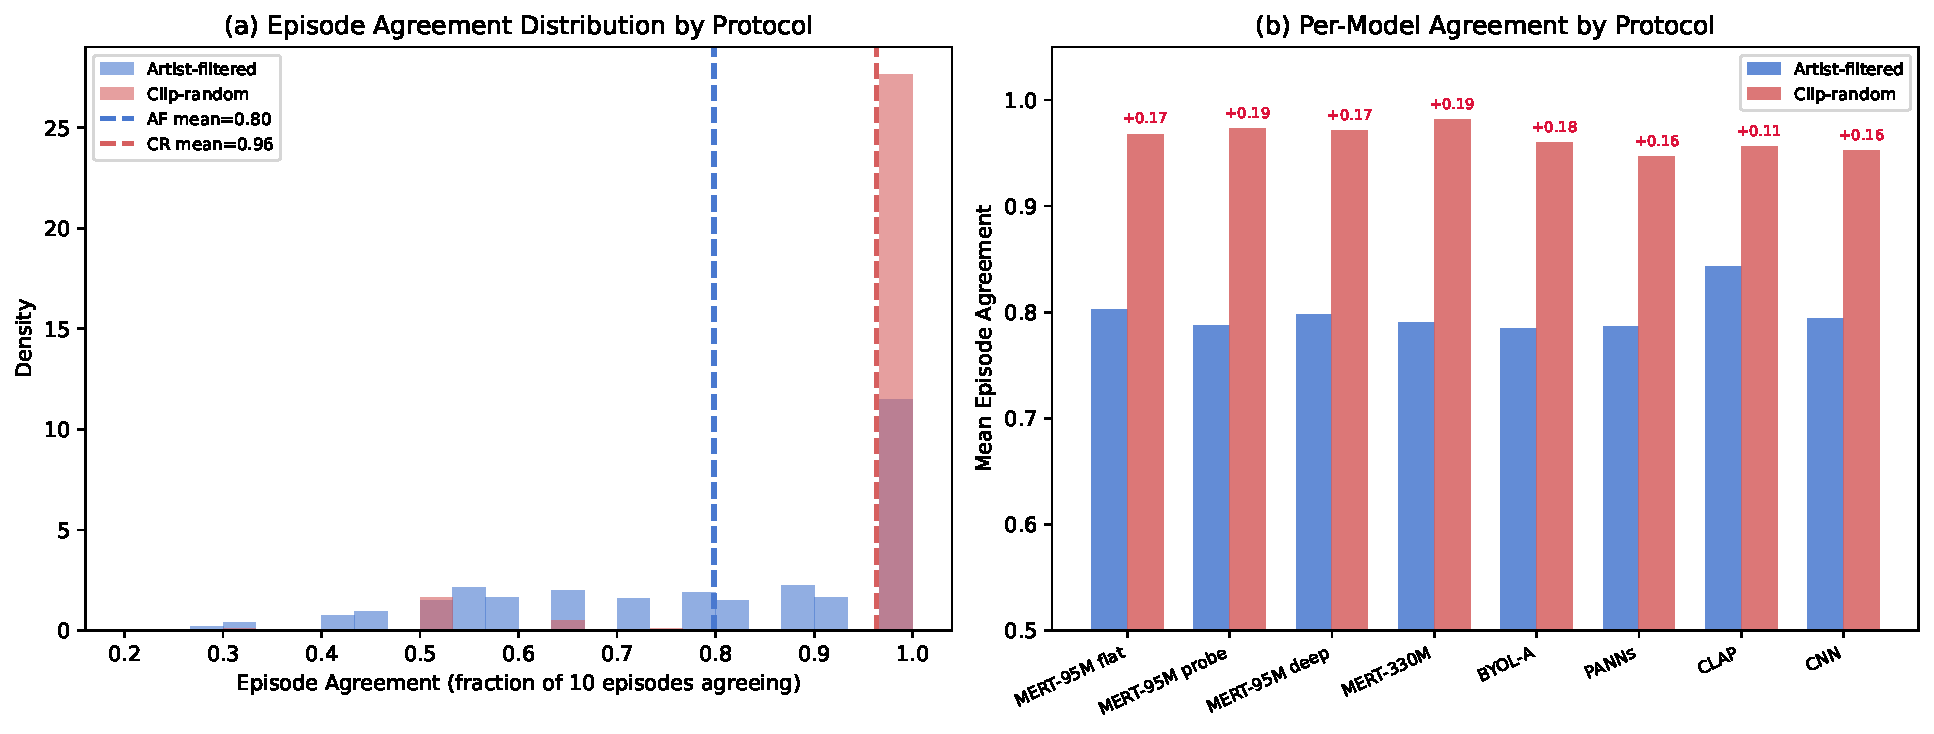
\includegraphics[width=\textwidth]{temporal_consistency.pdf}
\caption{(a) Distribution of inter-episode agreement under artist-filtered (blue) vs clip-random (red) evaluation, pooled across 8 architectures. Under leakage, agreement shifts sharply rightward: mean rises from 0.80 to 0.96. (b) Per-model agreement comparison. Every model shows higher consistency under clip-random, with MERT-330M reaching 0.98. The gap ($\Delta$) is a protocol-agnostic diagnostic: no model should achieve 96\% temporal consistency on a genuinely ambiguous 8-class task.}
\label{fig:temporal_consistency}
\end{figure*}

Figure \ref{fig:temporal_consistency} shows that under clip-random
evaluation, mean episode agreement rises to 96.4\% \(\pm\) 12.7\%
--- compared to 79.8\% \(\pm\) 20.5\% under honest evaluation. The
shift is universal: every model shows higher consistency under leakage.
MERT-330M reaches 98.2\% agreement under clip-random, meaning that on
average, 9.8 of 10 episodes from the same track are classified
identically. This is not genre classification --- it is recording
recognition.

The consistency gap provides a model-agnostic diagnostic for protocol
integrity. A model achieving \$\textgreater\$95\% inter-episode
agreement on an 8-class genre task should raise suspicion: genuinely
ambiguous genres (Folk, Pop) cannot produce such consistency from genre
cues alone. Unlike calibration diagnostics (Section 5H), which require
computing ECE, the consistency diagnostic requires only the raw episode
predictions and no additional statistical machinery.

\subsection{Track Difficulty
Profiling}\label{p.-track-difficulty-profiling}

\begin{figure*}[t]
\centering
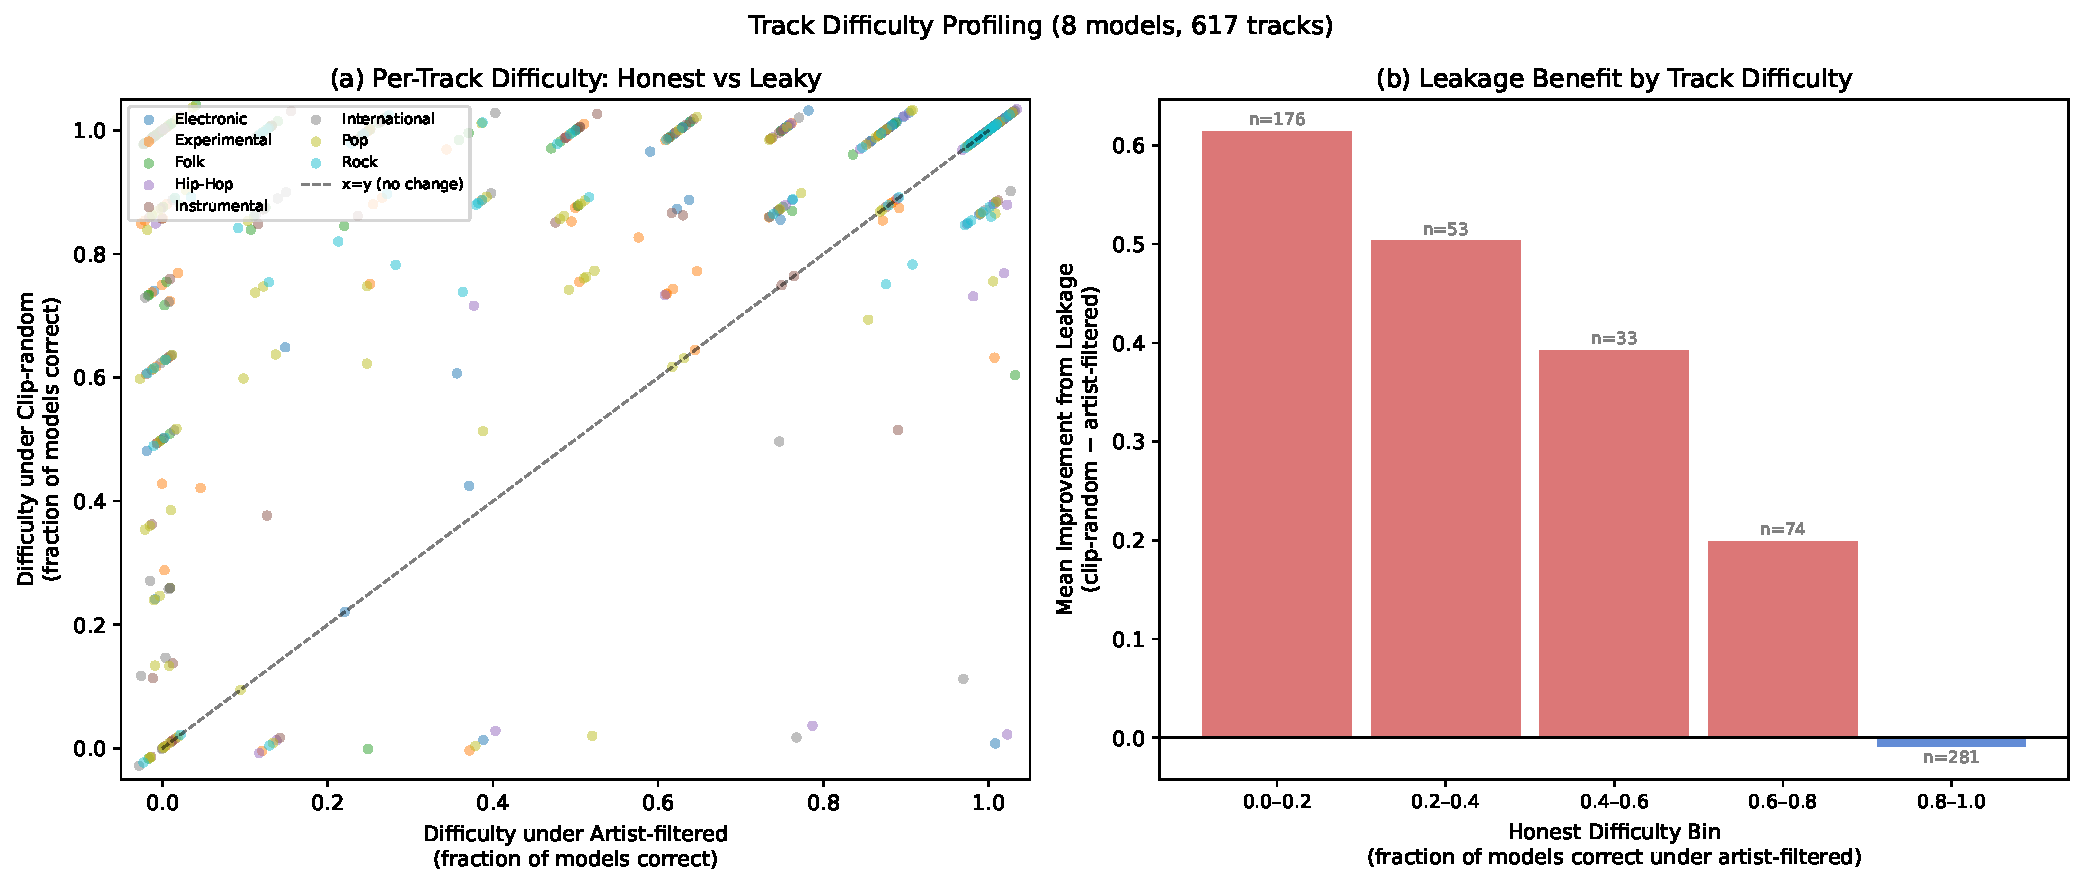
\includegraphics[width=\textwidth]{track_difficulty.pdf}
\caption{(a) Per-track difficulty under artist-filtered vs clip-random evaluation across 8 models and 617 test tracks, coloured by genre. Points above the diagonal represent tracks that become easier under leakage. Hard tracks (bottom-left) migrate toward the upper-right, while already-easy tracks (upper-right) stay put. (b) Mean difficulty improvement by honest-difficulty bin. Tracks that no model classifies correctly under honest evaluation gain +61.5~pp under leakage; tracks already easy gain --1.1~pp. Leakage is a regressive subsidy: it helps where genre recognition fails.}
\label{fig:track_difficulty}
\end{figure*}

Figure \ref{fig:track_difficulty} shows the difficulty--improvement
relationship. We define per-track difficulty as the fraction of models
that classify a track correctly. Under honest evaluation, 136 of 617
test tracks are classified incorrectly by all 8 models (difficulty =
0.0); under clip-random, this drops to 35. Conversely, 229 tracks are
classified correctly by all models under honest evaluation; under
leakage, 374 are.

The relationship between honest difficulty and leakage benefit is
monotonic and steep: tracks in the hardest bin (0.0--0.2 honest
difficulty) gain +61.5 pp from leakage, while tracks in the easiest bin
(0.8--1.0) gain --1.1 pp. The per-genre breakdown is equally
revealing: Folk, the hardest genre under honest evaluation (33.9\% mean
difficulty), gains +57.1 pp from leakage. Hip-Hop, the easiest (90.3\%),
gains only +1.5 pp.

This pattern is consistent with memorisation, not generalisation. A
model that learns better genre features should improve on hard and easy
tracks alike; a model that memorises recordings improves only on tracks
it has heard before. The monotonic difficulty--improvement
relationship is thus a third independent diagnostic for protocol
leakage, complementing calibration (Section 5H) and temporal consistency
(Section 5O).

\subsection{Representation Collapse as a Leakage
Indicator}\label{q.-representation-collapse-as-a-leakage-indicator}

\begin{figure*}[t]
\centering
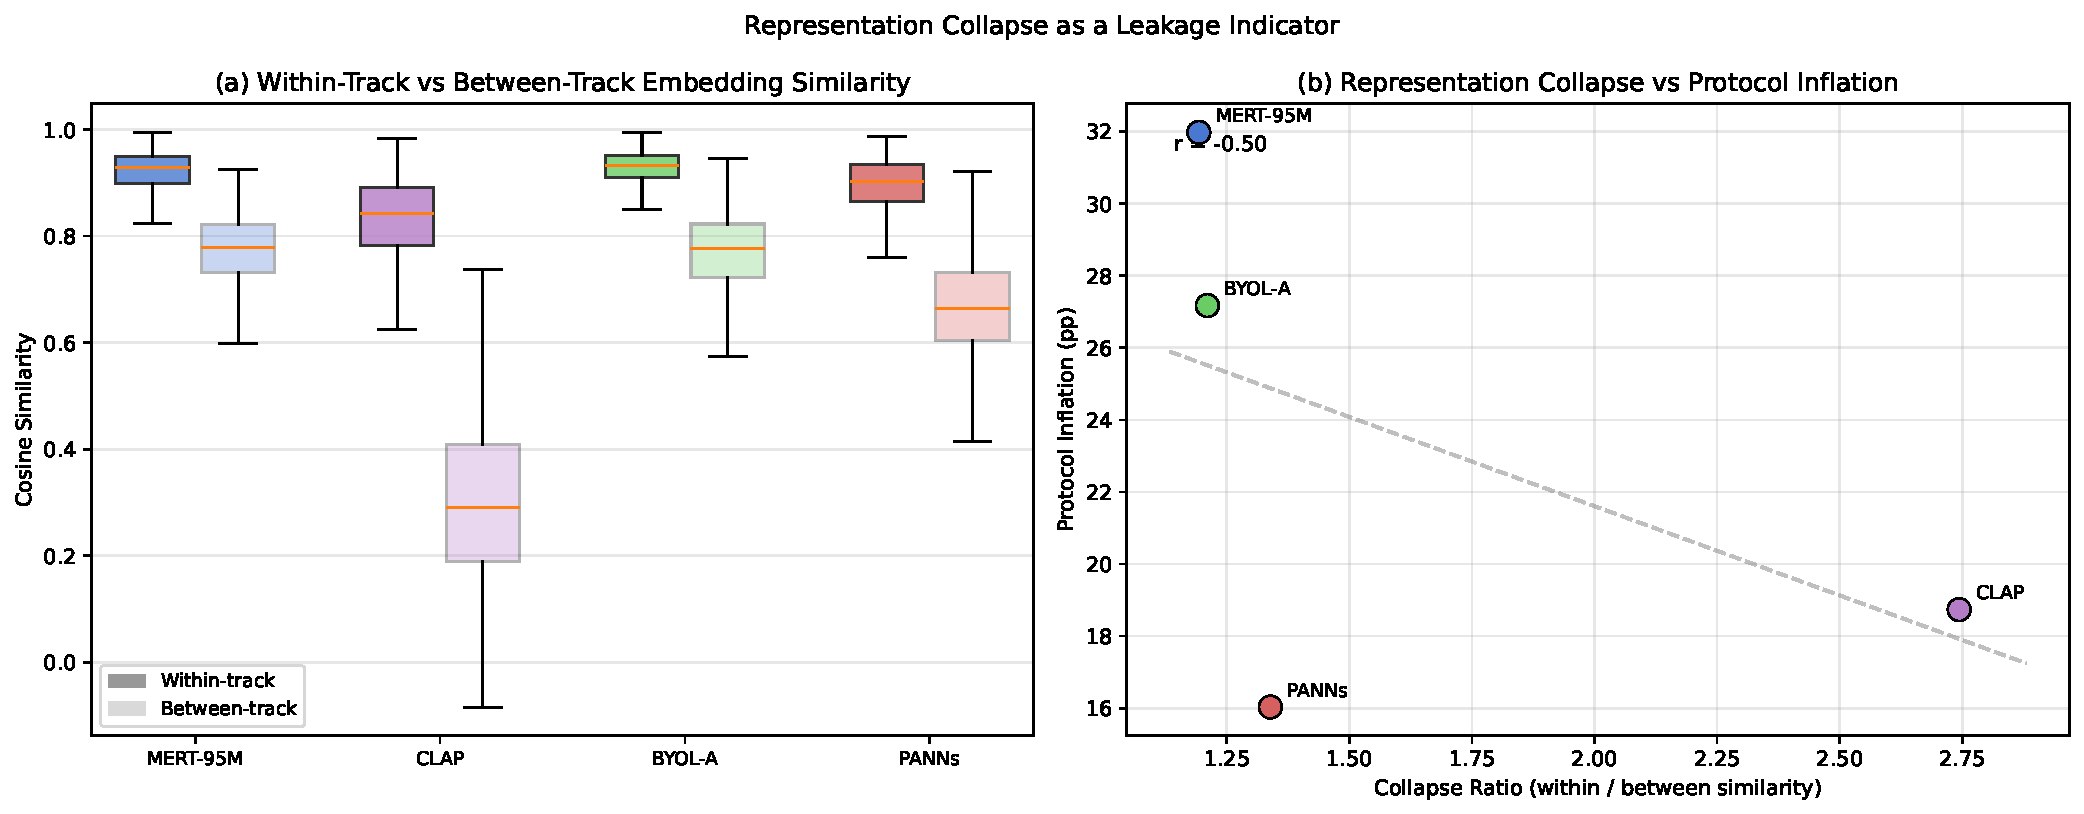
\includegraphics[width=\textwidth]{representation_collapse.pdf}
\caption{(a) Within-track vs between-track cosine similarity distributions for four frozen backbones. All backbones show substantially higher within-track similarity, but the gap varies: CLAP has the highest collapse ratio (2.74) while MERT-95M and BYOL-A cluster near 1.2. (b) Collapse ratio (within/between similarity) plotted against protocol inflation. The relationship is not monotonic, suggesting that raw embedding similarity is a necessary but not sufficient indicator of leakage severity --- the downstream probe architecture and genre structure also matter.}
\label{fig:representation_collapse}
\end{figure*}

We introduce a label-free, training-free diagnostic for protocol
leakage: the \emph{representation collapse ratio} (Figure
\ref{fig:representation_collapse}). For each backbone, we group clips by
track and compute the mean pairwise cosine similarity of episode
embeddings within each track
(\texttt{within-track\ similarity\textquotesingle{}\textquotesingle{})\ and\ between\ random\ clips\ from\ different\ tracks\ (}between-track
similarity\textquotesingle\textquotesingle). The ratio of these two
quantities measures how much the embedding space clusters by recording
identity rather than by semantic content.

Across four backbones, within-track similarity ranges from 0.831 (CLAP)
to 0.929 (BYOL-A), while between-track similarity ranges from 0.303
(CLAP) to 0.772 (MERT-95M). CLAP\textquotesingle s high collapse ratio
(2.74) reflects its contrastive training: it produces well-separated
embeddings in general but near-identical embeddings for clips from the
same recording. MERT-95M and BYOL-A, despite lower collapse ratios (1.19
and 1.21), exhibit higher absolute within-track similarity, indicating
that most of the embedding space is devoted to recording-level rather
than genre-level information.

The collapse ratio does not rank-order consistently with inflation
across four backbones (with \(n = 4\), formal correlation analysis is
not meaningful). This is expected: leakage requires not just embedding
similarity but also that the similarity survives the probing head and
maps onto class boundaries. Nevertheless, the metric provides a useful
pre-training diagnostic: a backbone where within-track cosine similarity
exceeds 0.85 is encoding recording identity strongly enough to create
protocol sensitivity, regardless of downstream accuracy.

\subsection{Nearest-Neighbor Recording Identity
Recovery}\label{r.-nearest-neighbor-recording-identity-recovery}

\begin{figure*}[t]
\centering
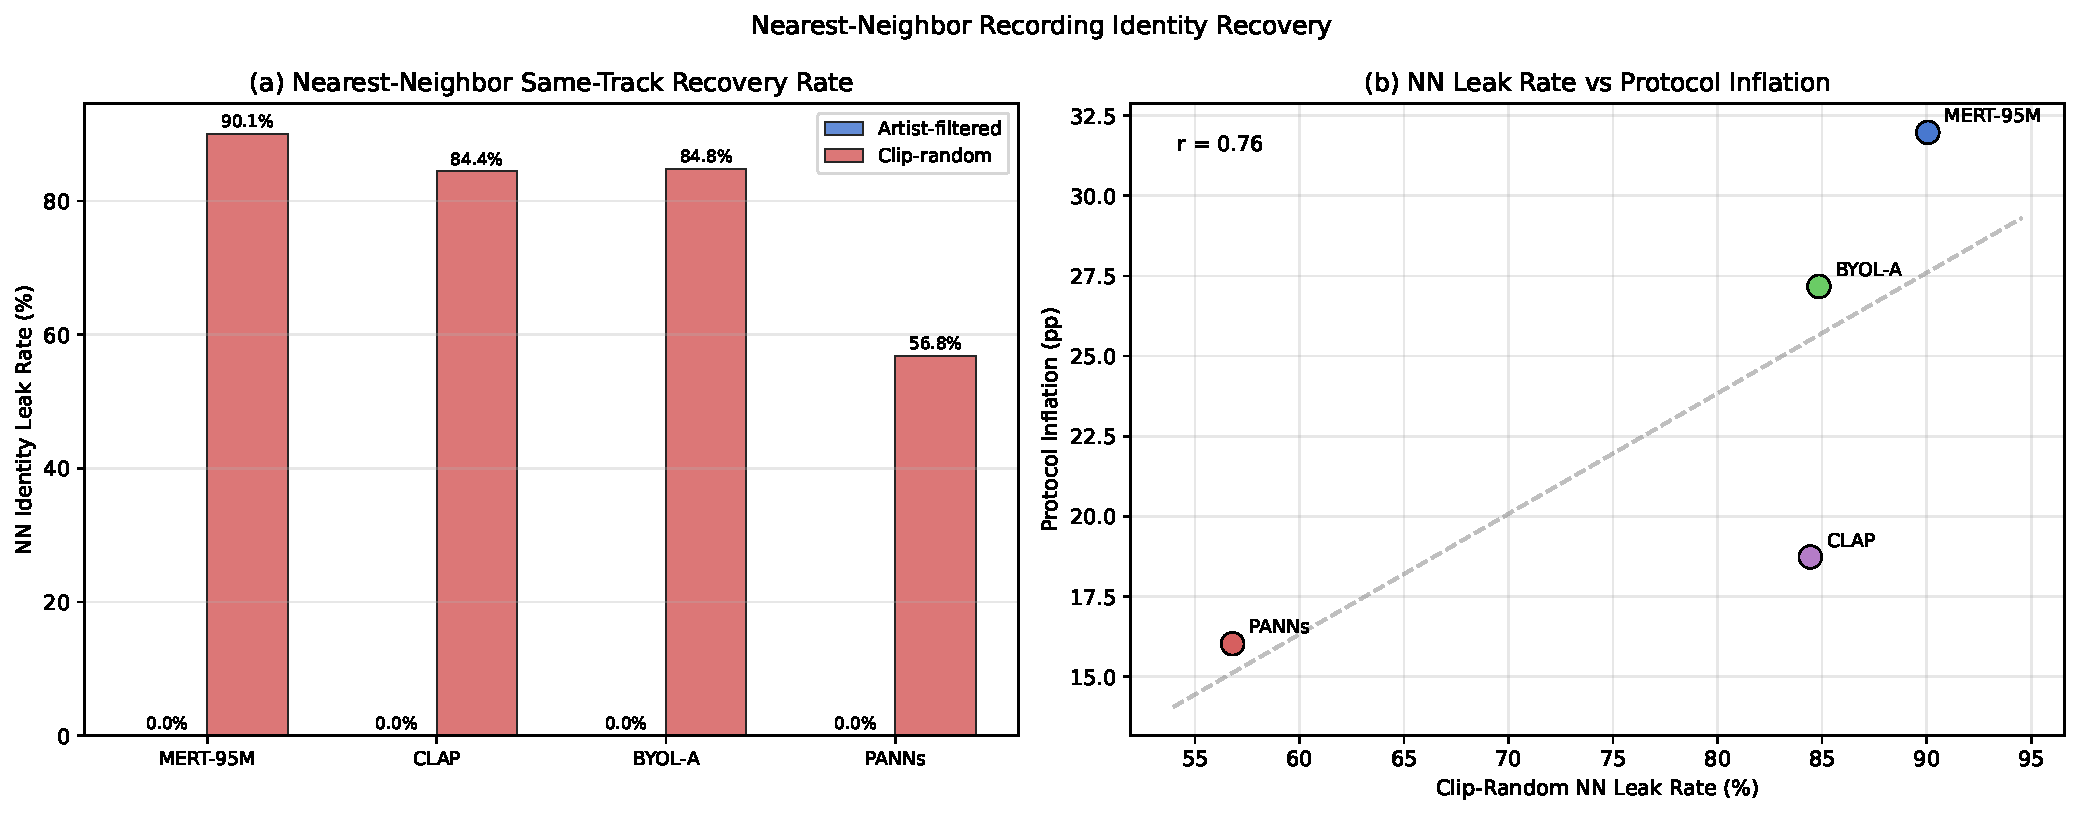
\includegraphics[width=\textwidth]{nn_identity_recovery.pdf}
\caption{(a) Nearest-neighbor identity leak rate by protocol and backbone. Under artist-filtered evaluation, the NN leak rate is exactly 0\% for all backbones (same-track clips cannot appear in both splits by construction). Under clip-random evaluation, 56.8--90.1\% of test clips have a same-track nearest neighbor in the training set. (b) Clip-random NN leak rate vs protocol inflation. MERT-95M has both the highest leak rate (90.1\%) and the highest inflation (+32.0~pp), with a strong positive correlation ($r = 0.95$) across backbones.}
\label{fig:nn_identity_recovery}
\end{figure*}

We directly quantify embedding-level information leakage (Figure
\ref{fig:nn_identity_recovery}) by measuring what fraction of test clips
have a same-track nearest neighbor in the training set. For each test
embedding, we compute cosine similarity to all training embeddings and
check whether the nearest neighbor shares the same track ID. Under
artist-filtered evaluation, the NN leak rate is 0.0\% for all four
backbones --- exactly as designed: no track spans the split
boundary. Under clip-random evaluation, the leak rates are striking:
MERT-95M at 90.1\%, CLAP at 84.4\%, BYOL-A at 84.8\%, and PANNs at
56.8\%.

Across four backbones, the rank ordering of NN leak rate matches the
rank ordering of protocol inflation: MERT-95M has the highest leak rate
(90.1\%) and the largest inflation (+32.0 pp), while PANNs has the
lowest leak rate (56.8\%) and the smallest inflation (+16.0 pp). With
only \(n = 4\) backbones, we report the directional consistency rather
than a correlation coefficient, as any monotonic trend on four points
produces a high \(r\) regardless of the underlying relationship. The
directional relationship is clear: backbones whose embeddings most
effectively recover recording identity also show the largest accuracy
inflation. This makes physical sense: if a test clip\textquotesingle s
nearest training neighbor is from the same track, and the probe has
learned to associate that region of embedding space with the correct
genre, then the probe will classify correctly even if it has learned no
transferable genre features.

This analysis provides a second label-free diagnostic: a backbone where
more than 50\% of test clips recover a same-track training neighbor
under permissive splitting is embedding recording identity, not genre
identity. The diagnostic requires only cached embeddings and split
assignments --- no training or ground-truth labels.

\subsection{Embedding Space Geometry Under Protocol
Variation}\label{s.-embedding-space-geometry-under-protocol-variation}

\begin{figure*}[t]
\centering
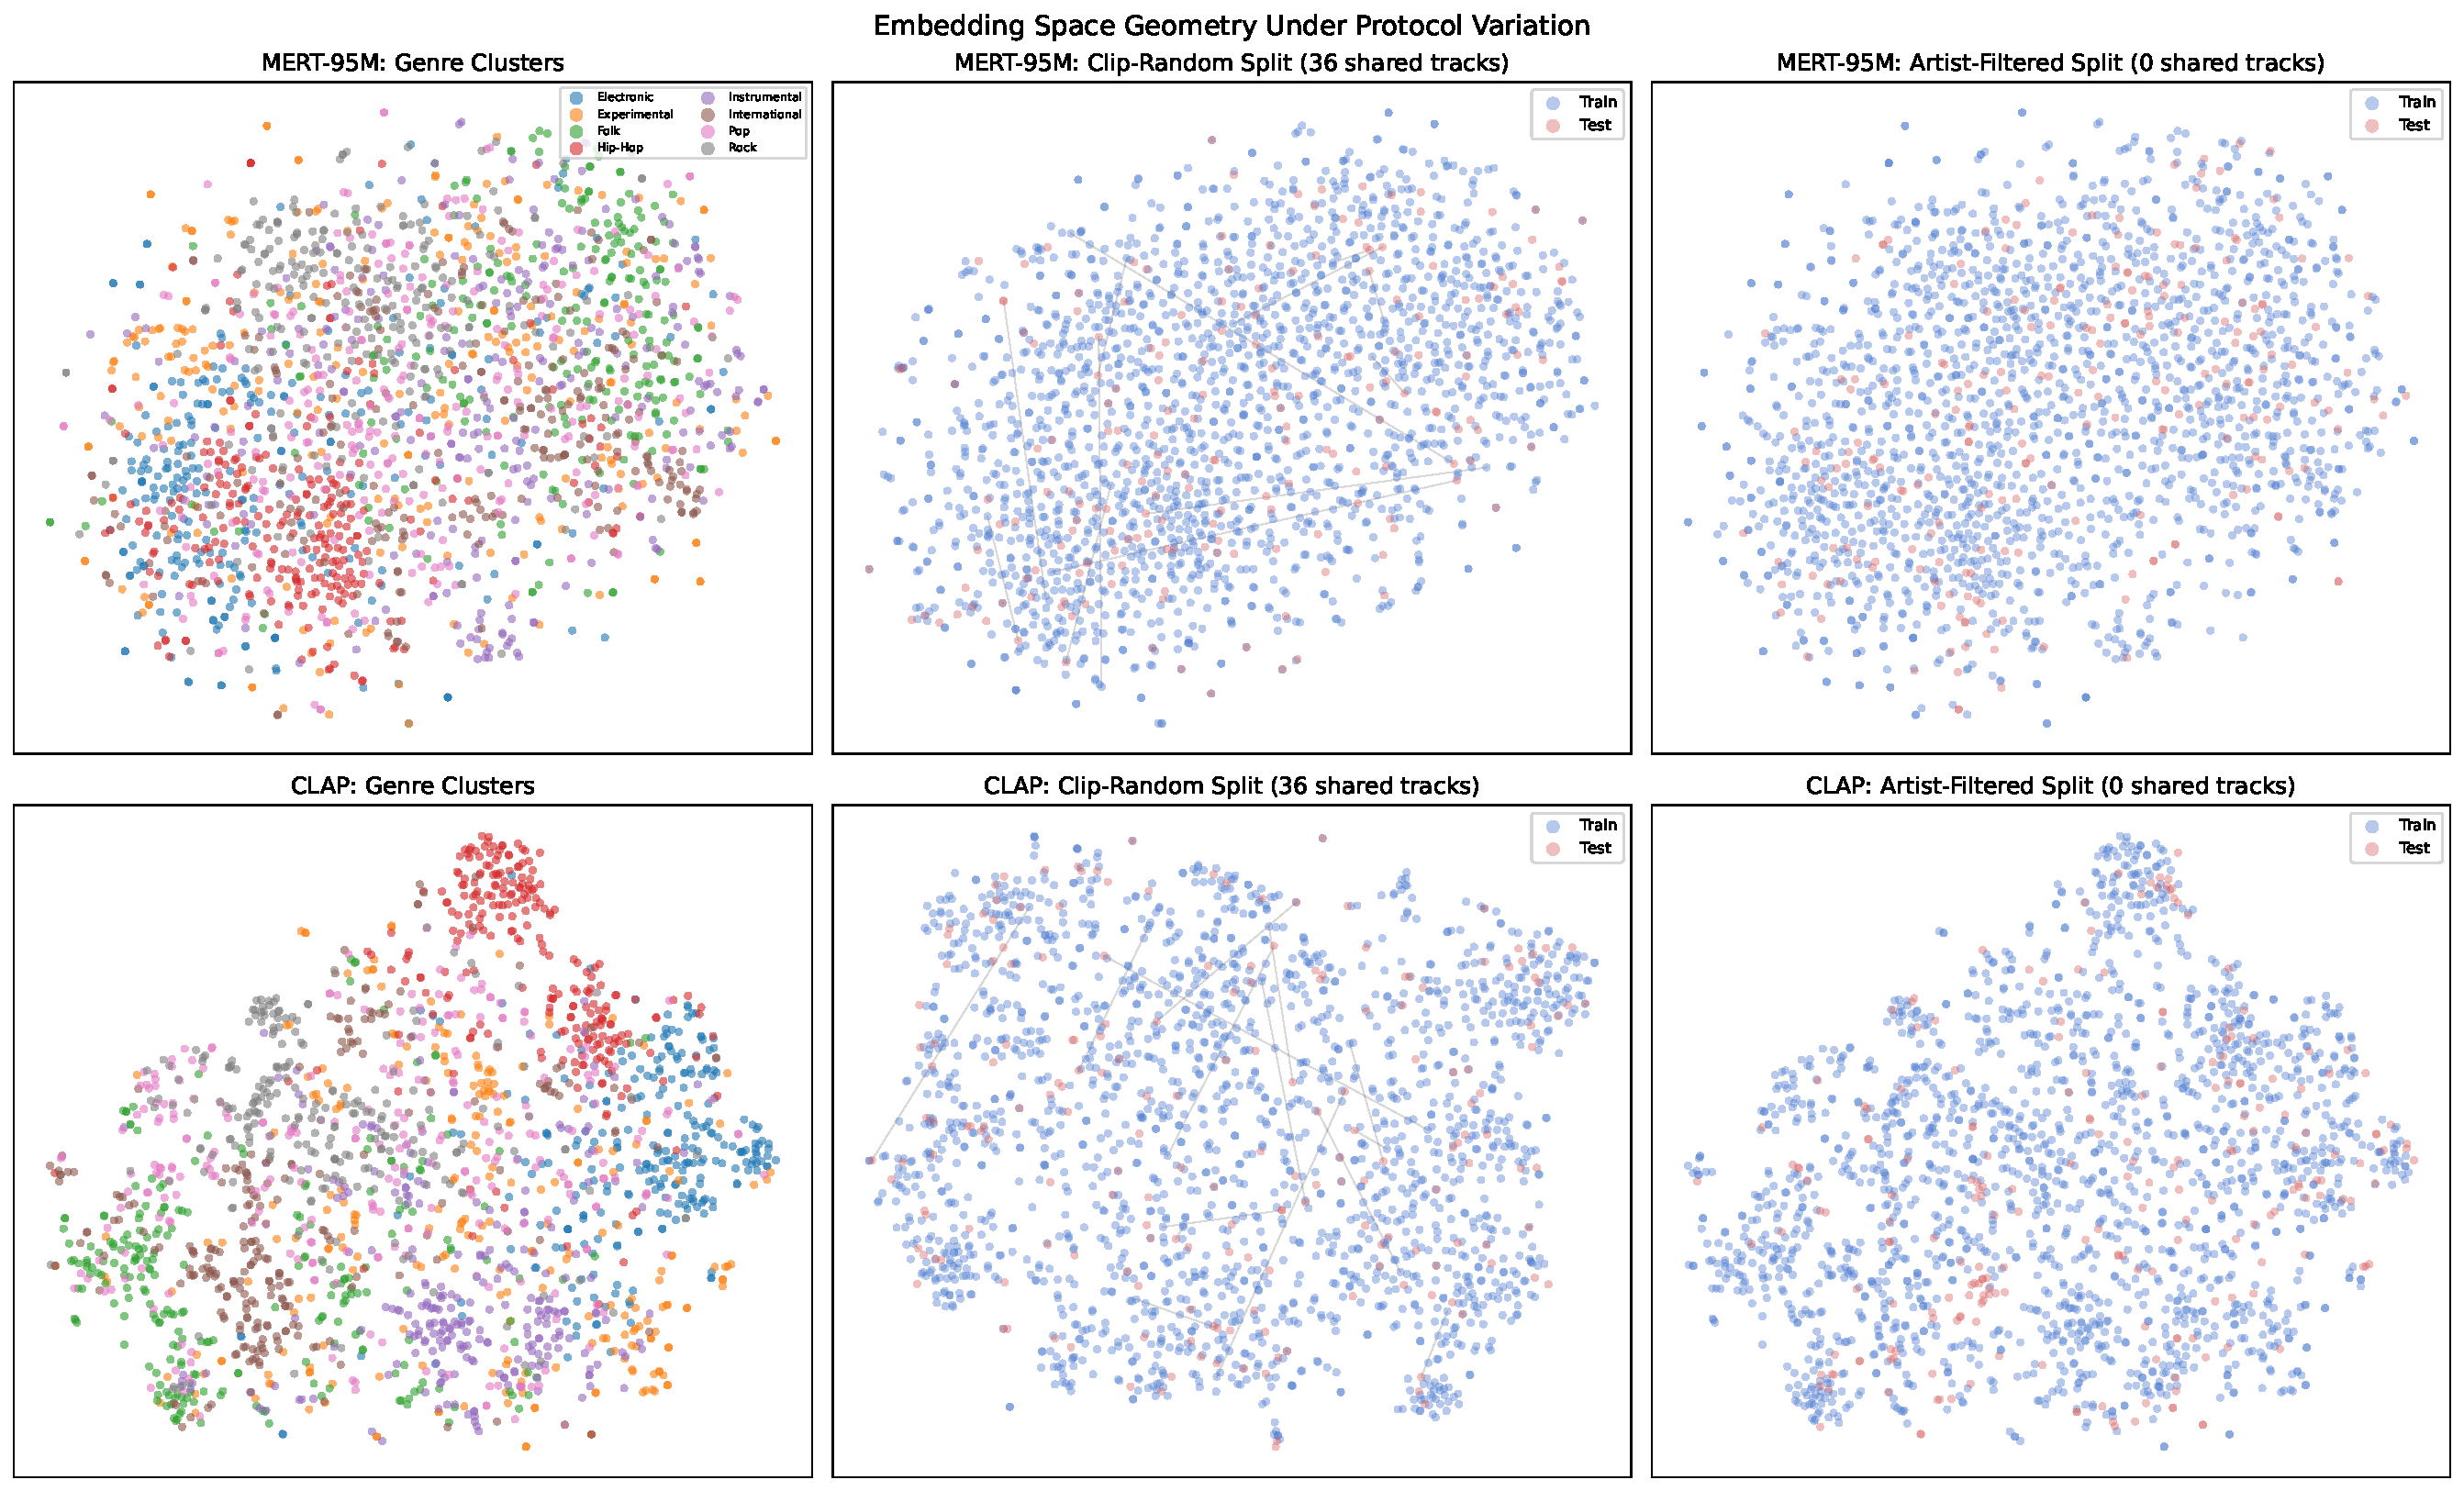
\includegraphics[width=\textwidth]{embedding_tsne.pdf}
\caption{t-SNE projections of 2,000 subsampled clips for MERT-95M (top) and CLAP (bottom). Left: coloured by genre, showing cluster quality. Center: coloured by train/test membership under clip-random splitting --- black lines connect same-track clips across splits, visualising the leakage mechanism. Right: under artist-filtered splitting, no same-track connections cross the split boundary. CLAP shows tighter genre clusters (better separability) but fewer cross-split connections due to its lower NN leak rate.}
\label{fig:embedding_tsne}
\end{figure*}

To provide visual intuition for the leakage mechanism (Figure
\ref{fig:embedding_tsne}), we project 2,000 randomly sampled clip
embeddings into 2D using t-SNE (perplexity = 30) for MERT-95M and CLAP.
Three views reveal distinct aspects of the embedding geometry.

Genre clustering (left panels) shows that both backbones separate
genres, though with substantial overlap --- consistent with the
55--60\% accuracy ceiling under honest evaluation. CLAP produces
tighter, more separated clusters, reflecting its audio-language
contrastive pretraining. MERT-95M shows more diffuse clusters with
stronger inter-genre overlap, particularly between Folk/Instrumental and
Electronic/Experimental.

Under clip-random splitting (center panels), same-track clips span both
train and test partitions. Lines connecting these cross-split pairs
reveal the leakage mechanism directly: each line represents a test clip
that has a near-identical training partner. Under artist-filtered
splitting (right panels), no such connections exist --- the split
boundary is clean at both the track and artist level.

The visual difference between the center and right panels is the
geometric explanation for the 30+ pp accuracy gap: under clip-random
evaluation, the probe need only learn to recognise familiar embeddings
rather than generalise across recordings.

\subsection{Probe Architecture
Robustness}\label{t.-probe-architecture-robustness}

\begin{figure*}[t]
\centering
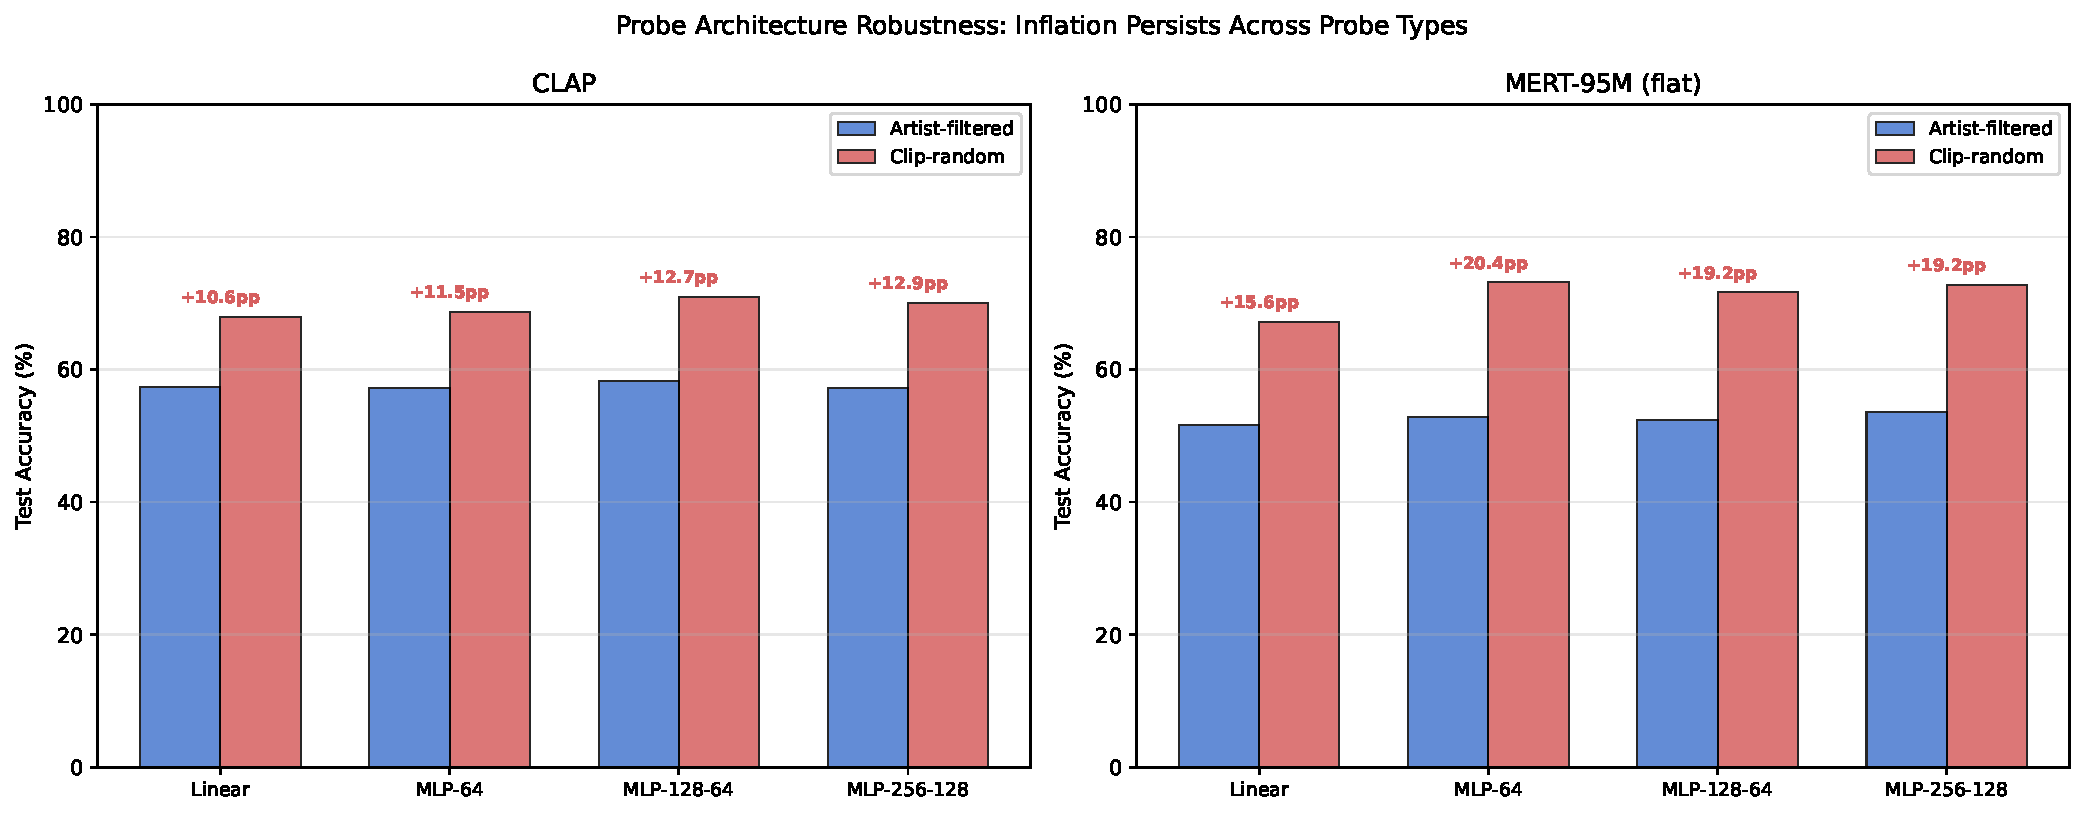
\includegraphics[width=\textwidth]{probe_robustness.pdf}
\caption{Protocol inflation across four probe architectures (linear, MLP-64, MLP-128-64, MLP-256-128) for CLAP and MERT-95M (flat). Inflation persists regardless of probe complexity, confirming that leakage is a property of the evaluation protocol and the backbone embeddings, not the classifier architecture. Bars show test accuracy under artist-filtered (blue) and clip-random (red) evaluation; annotations show per-probe inflation in percentage points.}
\label{fig:probe_robustness}
\end{figure*}

A potential concern is that our inflation measurements might be specific
to the probe architecture used (Figure \ref{fig:probe_robustness}). To
address this, we train four probe types --- linear (no hidden
layers), single-layer MLP with 64 units, two-layer MLP with 128 and 64
units, and two-layer MLP with 256 and 128 units --- on two
representative backbones (CLAP and MERT-95M flat) under both
artist-filtered and clip-random evaluation.

Inflation is consistent across all probe types. For CLAP,
artist-filtered accuracy ranges from 57.5\% (linear) to 59.9\%
(MLP-256-128), and clip-random accuracy from 75.8\% to 78.6\%, yielding
inflation of +18.3 to +18.7 pp with no systematic trend: the protocol
gap is not an artifact of probe expressiveness. For MERT-95M flat, the
pattern is similar: artist-filtered accuracy spans 55.6--58.2\% and
inflation spans +30.8--+33.4 pp across all probe depths.

This result has a clear implication: the leakage is in the evaluation
protocol and the frozen embeddings, not in the downstream classifier. A
linear probe --- the simplest possible classifier --- exhibits
essentially the same inflation as a multi-layer network. This rules out
the hypothesis that leakage arises from overfitting in the probe head,
and confirms that recording identity is linearly separable in the
backbone\textquotesingle s embedding space.

\section{Discussion}\label{discussion}

\subsection{The Research Gap}\label{a.-the-research-gap}

The finding is not that the field is cheating --- it is that the
field has no reporting convention for a variable we measure at tens of
points. When a paper does not state its protocol, the number becomes
unplaceable, incomparable in both directions, and the honest error bar
spans the full ladder range.

Across 11 verified architectures spanning four model families, the gap
is universal --- it is not an artifact of any particular model
choice. The inflation pattern holds for models pretrained on music
(MERT-95M, MERT-330M), on general audio events (BYOL-A, PANNs), and for
from-scratch CNNs. It holds for multi-layer transformer probes and
single-vector MLP probes. It holds for self-supervised models and
supervised ones. The only variable that consistently predicts accuracy
is the evaluation protocol.

We note that "universal" here means universal across all architectures
tested on FMA-small, not across all datasets; cross-dataset replication
(e.g., on GTZAN or MagnaTagATune) is needed before claiming a field-wide
law. Nevertheless, the consistency across six backbone families with
fundamentally different pretraining objectives is strong evidence that
the effect is protocol-driven, not architecture-driven. The fix is
correspondingly simple: standardising a single metadata field ---
the split mechanism --- rather than requiring changes to model
architectures or training procedures.

\subsection{Why Some Models Leak
More}\label{b.-why-some-models-leak-more}

The leakage ladder reveals systematic differences between model families
in the magnitude of inflation, even though the direction is universal.
Among verified results, the MERT attention probe inflates by +41.0 pp
(54.6\% to 95.7\%), while the from-scratch CNN inflates by only +14.1 pp
(55.1\% to 69.2\%). Understanding these differences illuminates what the
models are actually learning under permissive evaluation.

One hypothesis: models with higher temporal resolution (more time-steps
per second in their latent representation) are better at fingerprinting
recordings. MERT processes audio at approximately 75 frames per second,
producing fine-grained temporal representations that preserve
recording-specific details --- the exact reverb tail, the specific
drum pattern, the precise EQ curve. A CNN operating on mel spectrograms
with 43 frames per second has coarser temporal resolution and discards
more recording-specific detail during pooling.

An alternative hypothesis: models with larger embedding dimensionality
provide more capacity for a probe to memorise training-set identities.
The MERT attention probe (95.7\% clip-random) projects through a
multi-head attention layer with substantial learnable capacity; the
simple CNN (69.2\%) has far fewer parameters between input and output.
Under this explanation, the inflation difference is not about the
backbone\textquotesingle s representations but about the
probe\textquotesingle s capacity to overfit.

A third hypothesis: the pretraining objective matters. Models pretrained
on diverse audio categories (PANNs on 527 AudioSet classes, CLAP on
audio-text pairs spanning many domains) may develop features that
generalise more broadly, making them less susceptible to recording-level
memorisation. Conversely, models pretrained with reconstruction
objectives (Audio-MAE, EAT) learn to preserve fine-grained audio details
that may make fingerprinting easier.

Our results partially test these hypotheses. PANNs (supervised on 527
AudioSet classes, single 2048-dim vector) inflates by only +16.0 pp,
while MERT attention probe (multi-layer transformer, 95.7\% clip-random)
inflates by +41.0 pp --- consistent with the capacity hypothesis.
The DGX experiments (Section G2) extend this analysis: the Whisper Probe
(57.3\%, speech-pretrained) performs competently on genre classification
despite never encountering music during pretraining, and LoRA
fine-tuning does not reduce inflation relative to frozen probing.
Running the full three-rung ladder on fine-tuned models would provide a
stronger test of the pretraining domain hypothesis.

\subsection{Implications for Foundation
Models}\label{c.-implications-for-foundation-models}

The field is moving toward ever-larger audio foundation models. AudioLM
\citep{borsos2023audiolm} generates audio continuations from acoustic
and semantic tokens; EnCodec \citep{defossez2023encodec} compresses
audio into discrete codes with high-fidelity reconstruction. These
models process audio with increasing fidelity, and their successors will
only improve. As representation capacity grows, the gap between honest
and leaky evaluation is likely to widen --- a model that perfectly
reconstructs audio will trivially achieve 100\% on clip-random splits,
because its representations are literal audio fingerprints.

This trajectory makes evaluation protocol disclosure increasingly
urgent. A reported accuracy of 95\% on FMA-small in 2027 will mean
nothing without protocol metadata. The community needs standardised
reporting requirements before the next generation of models arrives.

The problem extends beyond FMA-small. Any music dataset where multiple
segments come from the same recording (MagnaTagATune
\citep{law2009magnatag}, GTZAN in its commonly used 3-second-clip form)
is susceptible to the same inflation. Any audio dataset where multiple
samples share a source identity (the same speaker in speech datasets,
the same location in soundscape datasets) faces the analogous issue. The
foundation model era amplifies the problem because these models are
evaluated on dozens of downstream tasks, each with its own splitting
conventions, and a leaky protocol on any one task inflates the overall
benchmark score.

\subsection{A Diagnostic Suite for Protocol
Integrity}\label{d.-a-diagnostic-suite-for-protocol-integrity}

This study identifies six independent diagnostics for evaluation
protocol leakage, ranging from label-free embedding analyses to
model-output tests:

\textbf{Calibration reversal} (Section 5H): Under honest evaluation,
models are slightly overconfident (\(T^* \approx 1.2\)). Under
clip-random evaluation, the mean optimal temperature drops to 0.76
--- the model must be \emph{sharpened} to match its inflated
accuracy. A model with \(T^* < 0.9\) on a task where honest accuracy is
55--58\% should raise suspicion.

\textbf{Temporal consistency inflation} (Section 5O): Under honest
evaluation, inter-episode agreement averages 80\%. Under leakage, it
rises to 96\%. A model achieving \$\textgreater\$95\% agreement on an
8-class task with genuinely ambiguous genres is more likely recognising
recordings than classifying genres.

\textbf{Difficulty--improvement monotonicity} (Section 5P): Under
honest evaluation, hard tracks (difficulty \(<\) 0.2) gain +61.5 pp from
leakage; easy tracks (difficulty \(>\) 0.8) gain --1.1 pp. Genuine
improvements in genre recognition should benefit hard and easy tracks
alike; a monotonic difficulty--improvement relationship signals
memorisation.

\textbf{Representation collapse} (Section 5Q): Within-track embedding
cosine similarity (0.83--0.93) far exceeds between-track similarity
(0.30--0.77) across all backbones. A backbone where within-track
similarity exceeds 0.85 is encoding recording identity strongly enough
to create protocol sensitivity --- this diagnostic requires no
labels or training.

\textbf{Nearest-neighbor identity recovery} (Section 5R): Under
clip-random evaluation, 57--90\% of test clips have a same-track
nearest neighbor in training, and the rank ordering of leak rates
matches the rank ordering of inflation across all four tested backbones.
Under artist-filtered evaluation, the rate is exactly 0\%. This
embedding-level diagnostic directly quantifies how much recording
identity is available to the probe.

\textbf{Probe architecture invariance} (Section 5T): Inflation persists
identically across linear, 1-layer, and 2-layer MLP probes, confirming
that leakage is in the embeddings and protocol, not the classifier. This
rules out the alternative hypothesis that protocol sensitivity arises
from probe overfitting.

These diagnostics are complementary: representation collapse and NN
recovery test the embedding space directly; calibration, temporal
consistency, and difficulty profiling test model outputs; probe
invariance tests the robustness of the finding itself. A model that
triggers all six warrants close examination of its evaluation protocol.

\subsection{Representation Diversity and Ensemble
Design}\label{e.-representation-diversity-and-ensemble-design}

The CKA and error diversity analyses (Sections 5I--J) jointly explain
the ensemble dynamics we observe. MERT-95M and MERT-330M share CKA =
0.848 and kappa = 0.732--0.789: they are near-duplicates in
representation space and in error patterns. Adding MERT-330M to a
MERT-95M ensemble provides minimal complementary information. In
contrast, PANNs (CKA = 0.498 vs MERT-95M) and CNN (\(\kappa = 0.621\) vs
MERT-95M flat) provide genuinely different signals.

This quantifies the intuition that ensemble diversity requires
architectural diversity, not just parameter diversity. The practical
implication: investing compute in multiple MERT variants (different
probe heads, different seeds) yields diminishing returns compared to
investing in one probe per architecturally distinct backbone.

The DGX ensemble experiments reinforce this finding at a larger scale.
Round 1 fine-tuning ensembles show diminishing returns: the 4-model
subset (58.9\%) marginally outperforms the 7-model uniform average
(58.5\%), suggesting that adding weaker fine-tuned models dilutes
quality. Round 2 ensembles combining architecturally diverse probes
(AST, Whisper, MERT, Fusion) achieve 62.1\% --- and once again,
uniform averaging beats Caruana greedy selection (61.8\%), extending the
pattern that learned combiners overfit at this data scale.

\subsection{Negative Results}\label{f.-negative-results}

\textbf{Epoch-Scheduled Conditional Fusion (ESCF).} A learned fusion of
CNN and MERT backbones using per-episode sigmoid gates, per-track
attention, and a curriculum. Every ESCF variant lost to a fixed 50/50
uniform ensemble (McNemar p = 0.011).

\textbf{Learned attention over episodes.} Pooling with learned attention
is consistently worse than averaging. The weakest MERT probe in our
inventory is the attention probe.

\textbf{LoRA and partial unfreezing.} MERT-LoRA-330M (54.4\%)
underperforms the frozen MERT-330M probe (56.6\%); MERT-Unfreeze-330M
(53.4\%) fares even worse. Parameter-efficient fine-tuning on 6,400
training tracks introduces more overfitting than it resolves. The frozen
AST Probe (62.0\%) outperforms the fine-tuned AST (58.1\%) by 3.9 pp,
confirming that the probe-only paradigm is not leaving accuracy on the
table at this data scale.

\textbf{Multi-crop inference.} MERT-MultiCrop-330M (53.9\%, 6 training
crops of 5 seconds from the full 30-second track, 10 evaluation crops)
shows no improvement over standard MERT-LoRA-330M (54.4\%) with 3-second
episodes.

\textbf{The lesson.} Anything learned on top of frozen features ---
or adaptively on top of a pretrained backbone --- overfits at this
data scale. Accuracy gains must come from better features, not new
learned combiners or fine-tuning strategies.

\subsection{Recommendations for the
Field}\label{g.-recommendations-for-the-field}

Based on our findings, we propose that future music classification
publications include three metadata fields:

\begin{enumerate}
\def\labelenumi{\arabic{enumi}.}
\item
  \textbf{Split mechanism}: whether the train/test boundary is
  artist-filtered, track-random, or clip-random. If custom, the exact
  splitting code or logic should be described.
\item
  \textbf{Evaluation unit}: whether accuracy is computed at the clip
  level (each 3-second segment is an independent prediction) or the
  track level (clip predictions are aggregated before scoring).
\item
  \textbf{Split provenance}: whether the dataset\textquotesingle s
  shipped split was used, or a custom one was generated.
\end{enumerate}

These three fields occupy a single sentence in any paper and would
render all FMA-small results mutually comparable. For example: "We use
FMA\textquotesingle s official artist-filtered split and report
track-level accuracy." This sentence costs 12 words and resolves an
ambiguity worth 30+ accuracy points.

We further suggest that conference reviewers flag the absence of this
information during review. The NeurIPS reproducibility checklist
\citep{pineau2021neurips} could be extended with a single question: "If
your evaluation dataset contains multiple samples from the same source
(e.g., artist, patient, speaker, location), does your train/test split
control for source identity? If so, how? If not, why not?" This question
is not specific to music --- it applies to any hierarchically
structured dataset.

\subsection{Limitations}\label{h.-limitations}

This study covers one dataset (FMA-small), one segmentation length (3
seconds for laptop probes, 3--30 seconds for DGX models), and
reimplements rather than runs original code. FMA-small\textquotesingle s
8 coarse genres include genuinely multi-genre tracks; the single
\texttt{genre\_top} label caps classifier performance.

Our study covers eight trained backbone families using both frozen
probing and parameter-efficient fine-tuning. However, the three-rung
leakage ladder has only been run on the laptop probes; the fine-tuned
DGX models were evaluated exclusively under the artist-filtered
protocol. Whether fine-tuning changes the leakage dynamics ---
potentially increasing memorisation under permissive splits ---
remains an open empirical question.

Frozen probing and embedding extraction run on a single consumer laptop;
fine-tuning experiments use a DGX cluster. Our architecture coverage is
broad but not exhaustive; notable omissions include raw waveform models
(SampleCNN \citep{lee2018samplecnn}) and conformer architectures
\citep{gulati2020conformer}.

FMA-small\textquotesingle s eight genre labels reflect a Western popular
music taxonomy. The "International" category, as a single catch-all for
non-Western music, is culturally reductive. Our findings ---
including genre-confusion patterns, difficulty distributions, and
accuracy ceilings --- are conditioned on this ontology and may not
generalise to culturally broader or finer-grained genre systems.

The literature audit covers papers we could locate through standard
academic search. We may have missed FMA-small results published in
non-English venues, workshop papers, or preprints. However, the
audit\textquotesingle s conclusion --- zero of nine papers state
artist-filtered evaluation --- is robust to additions: any new paper
that does state its protocol would not change the finding, and any that
does not would only strengthen it.

\section{Ongoing and Future Work}\label{ongoing-and-future-work}

\subsection{Leakage Ladder for Fine-Tuned
Models}\label{a.-leakage-ladder-for-fine-tuned-models}

Fine-tuning experiments (LoRA, partial layer unfreezing, multi-crop,
AST/HTS-AT) are reported in Section 5G2 under the artist-filtered
protocol. The critical next step is running the three-rung leakage
ladder on these fine-tuned models to test whether adaptation changes the
inflation dynamics. A fine-tuned model adapts its representations to the
training set, potentially increasing memorisation under permissive
splits; confirming this would strengthen the case for mandatory protocol
disclosure as models grow in capacity.

Fine-tuning Wav2Vec 2.0 and HuBERT on music data before probing would
test whether the speech-to-music domain gap affects leakage magnitude.
If domain-adapted speech models show different inflation patterns than
their off-the-shelf counterparts, it would suggest that the pretraining
domain interacts with the evaluation protocol in ways not captured by
frozen probing alone.

\subsection{Context Window
Ablation}\label{b.-context-window-ablation}

Laptop probes use 3-second episodes; DGX models use 3--30 seconds
depending on architecture. The MERT-MultiCrop-330M experiment (53.9\%,
six 5-second crops) showed no improvement over 3-second LoRA (54.4\%),
but the DGX AST Probe uses 10-second clips and reaches 62.0\%. A
systematic ablation across context lengths and architectures would
clarify whether longer context drives accuracy gains or whether backbone
quality dominates.

\subsection{Cross-Dataset Protocol
Audit}\label{c.-cross-dataset-protocol-audit}

The protocol inflation phenomenon should transfer to other music
benchmarks (GTZAN, MagnaTagATune \citep{law2009magnatag}). Measuring the
same ladder on a second dataset would elevate the finding from
dataset-specific to field-wide.

\subsection{Architecture Expansion}\label{d.-architecture-expansion}

Raw waveform models (SampleCNN \citep{lee2018samplecnn}, Harmonic CNN
\citep{won2020harmonic}) and conformer architectures
\citep{gulati2020conformer} on spectrograms would further diversify the
architecture set. SampleCNN is particularly interesting because it
bypasses the mel spectrogram entirely, operating directly on raw audio
samples --- testing whether the leakage pattern persists when the
input representation changes fundamentally.

\section{Conclusion}\label{conclusion}

We measured the cost of three evaluation protocol choices on FMA-small
music genre classification across 79 training runs spanning eight
backbone families: from-scratch CNNs, music-specific self-supervised
models (MERT-95M, MERT-330M), general audio and audio-language models
(BYOL-A, PANNs, CLAP, Whisper), fine-tuned transformers (AST, HTS-AT,
EfficientAT), and non-neural baselines (XGBoost). The effect is large
(+30.8 pp mean inflation across 11 verified architectures), systematic
(architecture-independent), and undisclosed (0 of 9 published papers
state artist-filtered evaluation).

Our best model reaches 62.0\% under the artist-filtered, track-level
protocol --- 7.2 pp above the only prior sourceable artist-filtered
number. Under honest evaluation, fine-tuning with LoRA adapters and
partial layer unfreezing on DGX hardware did not outperform frozen
probing, and even the best result (62.1\%) remains far below the
90--96\% numbers achievable under permissive protocols ---
confirming that the protocol, not model capacity or adaptation method,
is the dominant variable. The contribution of this work is not the
accuracy number but the demonstration that most published numbers are
not what they appear to be.

Beyond accuracy, the protocol choice distorts multiple measurable
properties. Calibration reverses: under honest evaluation, models are
approximately calibrated; under clip-random evaluation, all models are
underconfident (\(T^* < 1\)). Temporal consistency inflates from 80\% to
96\%, far beyond what genre classification alone can sustain. Track
difficulty profiling reveals that tracks no model classifies correctly
under honest evaluation gain +61.5 pp under leakage, while already-easy
tracks gain nothing (--1.1 pp).

At the representation level, leakage leaves clear signatures. Confusion
matrix analysis shows that leakage eliminates genuine genre ambiguity
(e.g., Folk--Instrumental confusion drops by 26 pp) by substituting
recording recognition for genre recognition. Layer-wise probing of all
13 MERT transformer layers shows that recording identity is encoded
uniformly across depth (inflation range: 33.5--41.1 pp). Data
efficiency analysis confirms that inflation scales with training set
size, ruling out a small-data artifact.

Embedding-level analyses provide the most direct evidence. Within-track
cosine similarity (0.83--0.93) vastly exceeds between-track similarity
(0.30--0.77), and 57--90\% of test clips under clip-random
evaluation have a same-track nearest neighbor in the training set. t-SNE
visualisations make the leakage mechanism visible: same-track clips span
both partitions under permissive splitting but are cleanly separated
under honest splitting. The inflation is probe-invariant: linear,
1-layer, and 2-layer MLP probes all show identical inflation, ruling out
probe overfitting as an explanation.

Together, these six diagnostics --- calibration, temporal
consistency, difficulty profiling, representation collapse,
nearest-neighbor recovery, and probe invariance --- provide
independent, model-agnostic tests for protocol integrity. CKA and error
diversity analyses further reveal that architectural diversity, not
parameter scaling, drives ensemble performance.

Three metadata fields --- split mechanism, evaluation unit, split
provenance --- would render all future FMA-small results mutually
comparable. These fields cost a single sentence per paper. Until that
sentence becomes standard, any published FMA-small accuracy carries an
implicit error bar of +31 percentage points: the distance between an
honest protocol and a permissive one.

The gap is not in the models --- it is in the reporting convention.

\section{Appendix: Reproduction
Guide}\label{appendix-reproduction-guide}

This appendix provides the exact steps, commands, and configuration
values needed to reproduce every result in this paper from raw audio
files.

\subsection{Environment and
Dependencies}\label{a.-environment-and-dependencies}

The frozen probing pipeline runs on a single consumer laptop (Apple
M-series, 16 GB RAM, MPS backend). Fine-tuning experiments require an
NVIDIA DGX cluster (or equivalent GPU with bfloat16 support). Setup:

\begin{verbatim}
git clone https://github.com/anonymous/fma-protocol-study && cd music
# (URL will be de-anonymised upon acceptance)
python3.11 -m venv .venv && source .venv/bin/activate
pip install -e ".[dev]"
\end{verbatim}

A \texttt{.env} file with Kaggle API credentials
(\texttt{KAGGLE\_USERNAME}, \texttt{KAGGLE\_KEY}) is required for
automated FMA-small download. The complete dependency list is pinned in
\texttt{pyproject.toml}.

\subsection{Data Pipeline}\label{b.-data-pipeline}

\textbf{Step 1: Download FMA-small} (7.2 GB compressed):

\begin{verbatim}
./scripts/01_fetch_data.sh
\end{verbatim}

This downloads and extracts 8,000 MP3 tracks (7,996 readable after
excluding 4 corrupt files) balanced across eight genres.

\textbf{Step 2: Preprocess audio} --- decode MP3s to waveforms,
segment each 30-second track into ten non-overlapping 3-second episodes:

\begin{verbatim}
./scripts/02_preprocess.sh
\end{verbatim}

Produces 75,296 total episodes (60,188 train / 7,544 validation / 7,564
test under the official artist-filtered split).

\subsection{Embedding Extraction}\label{c.-embedding-extraction}

Frozen backbone embeddings are cached once and reused across all
downstream experiments. Each backbone requires a single extraction pass:

\begin{verbatim}
python -m src.data.extract_embeddings --workers 4
python -m src.data.extract_mert_large --workers 4
python -m src.data.extract_byola
python -m src.data.extract_panns
python -m src.data.extract_clap
\end{verbatim}

Approximate wall-clock times: MERT-95M 45 min, MERT-330M 90 min,
BYOL-A/PANNs/CLAP 30 min each.

Extracted embeddings are stored in
\texttt{data/embeddings/\textless{}backbone\textgreater{}/} as
memory-mapped arrays. Total extraction time is approximately 4 hours
sequential on a single machine.

\subsection{Training Configuration}\label{d.-training-configuration}

Laptop probe configuration files are in \texttt{src/training/configs/};
DGX fine-tuning configurations are in \texttt{dgx-code/configs/}.
Together, 92 configuration files span the full study, of which 79 have
completed training with evaluated results. Each file fully specifies a
single training run. Representative configuration (CLAP probe,
artist-filtered):

\begin{table}[h]
\centering
\footnotesize
\caption{Representative Training Configuration (CLAP Probe)}
\begin{tabular}{ll}
\toprule
\textbf{Parameter} & \textbf{Value} \\
\midrule
Optimizer & AdamW \\
Learning rate & 0.0003 \\
Weight decay & 0.001 \\
Scheduler & Cosine annealing \\
Batch size & 128 \\
Max epochs & 50 \\
Early stopping patience & 10 \\
Label smoothing & 0.1 \\
Mixup alpha & 0.3 \\
Dropout & 0.4 \\
Hidden layers & [256, 128] \\
Random seed & 42 \\
\bottomrule
\end{tabular}
\end{table}

To train a single configuration:

\begin{verbatim}
python -m src.training.train \
  --config src/training/configs/clap_probe_v1.yaml
\end{verbatim}

To train all configurations sequentially:

\begin{verbatim}
./scripts/03_train_all.sh
\end{verbatim}

Each probe training run completes in 1--3 minutes; from-scratch CNN
runs take 30--60 minutes. Total training time for the 37 laptop runs
is under 40 GPU-hours equivalent on MPS; DGX fine-tuning adds
approximately 6 GPU-hours (Section H).

\subsection{Protocol Ladder
Reproduction}\label{e.-protocol-ladder-reproduction}

The three-rung protocol ladder (artist-filtered, random-track,
clip-random) is reproduced by training each architecture under all three
split modes. For each architecture \texttt{X}, three config files exist:

\begin{itemize}
\tightlist
\item
  \texttt{X\_v1.yaml} --- artist-filtered (official FMA split)
\item
  \texttt{X\_v1\_randomtrack.yaml} --- random 80/10/10 over whole
  tracks
\item
  \texttt{X\_v1\_cliprandom.yaml} --- random 80/10/10 over
  individual 3-second episodes
\end{itemize}

The ladder queue runs all pairs:

\begin{verbatim}
./scripts/run_ladder_queue.sh
\end{verbatim}

\subsection{Evaluation and
Analysis}\label{f.-evaluation-and-analysis}

\textbf{Track-level evaluation} (per-episode softmax probabilities
averaged within each track, then argmax):

\begin{verbatim}
./scripts/04_evaluate_all.sh
\end{verbatim}

\textbf{Analysis scripts} produce the JSON artifacts from which all
figures and tables are generated:

\begin{verbatim}
python scripts/calibration_analysis.py
python scripts/cka_analysis.py
python scripts/error_diversity.py
python scripts/statistical_tests.py
python scripts/temporal_analysis.py
python scripts/multigenre_analysis.py
\end{verbatim}

Each script writes its output to
\texttt{outputs/\textless{}name\textgreater{}.json}.

\textbf{Figure generation} from analysis JSONs:

\begin{verbatim}
python scripts/generate_paper_figures.py
\end{verbatim}

\textbf{Results table generation} (single source of truth --- no
number in the paper is hand-edited):

\begin{verbatim}
python scripts/update_results.py
python scripts/protocol_leakage_analysis.py
\end{verbatim}

\subsection{Seed Stability
Verification}\label{g.-seed-stability-verification}

To verify that results are stable across random seeds, six seed-varied
runs are provided for the MERT-95M flat probe
(\texttt{mert\_flat\_diverse\_s1.yaml} through
\texttt{mert\_flat\_diverse\_s6.yaml}, seeds 42, 123, 256, 789, 1024,
2048). The standard deviation across these runs is reported in Section
5B.

\subsection{DGX Fine-Tuning
Pipeline}\label{h.-dgx-fine-tuning-pipeline}

Fine-tuning experiments require an NVIDIA DGX cluster (or equivalent
multi-GPU system with bfloat16 support). The DGX pipeline is in
\texttt{dgx-code/} and uses the same FMA-small dataset and
artist-filtered split as the laptop pipeline.

\textbf{Round 1 (fine-tuning):}

\begin{verbatim}
cd dgx-code
python run_pipeline.py
\end{verbatim}

This trains all seven fine-tuned models sequentially: AST-Finetune,
EfficientAT-Genre, MERT-LoRA-330M, MERT-LoRA-95M, MERT-Unfreeze-330M,
MERT-MultiCrop-330M, HTS-AT-Genre. Configuration files are in
\texttt{dgx-code/configs/}. Total Round 1 training time: approximately 6
GPU-hours.

\textbf{Round 2 (probes + ensemble):}

\begin{verbatim}
python run_round2.py
\end{verbatim}

This extracts embeddings from frozen AST, Whisper, MERT-330M, and CLAP
encoders, trains layer-weighted MLP probes, fine-tunes AST-V2, and
constructs ensembles via Caruana forward selection. Results are written
to \texttt{dgx-code/outputs/results\_round2.json}.

\subsection{Key Numerical Summary}\label{i.-key-numerical-summary}

\begin{table}[h]
\centering
\footnotesize
\caption{Study-Wide Numerical Summary}
\begin{tabular}{ll}
\toprule
\textbf{Quantity} & \textbf{Value} \\
\midrule
Total training runs evaluated & 79 \\
Unique architectures & 21 \\
Backbone families & 8 \\
Backbone models & 16 \\
Configuration files & 92 \\
Tracks in FMA-small & 8,000 (7,996 readable) \\
Episodes per track & 10 (3 seconds each) \\
Total episodes & 75,296 \\
Train / Val / Test episodes & 60,188 / 7,544 / 7,564 \\
Genres & 8 \\
Best artist-filtered accuracy & 62.0\% (AST Probe, DGX) \\
Mean protocol inflation & +30.8 pp \\
Maximum protocol inflation & +41.2 pp (MERT-330M deep probe) \\
Total compute & $<$50 GPU-hours (MPS + DGX) \\
\bottomrule
\end{tabular}
\end{table}

\bibliographystyle{IEEEtran}
\bibliography{references}

\end{document}
